
%NDSS
%\documentclass[conference]{IEEEtran}
%\pagestyle{plain}
%CHES
%CHES
\documentclass[submission]{iacrtrans}

\newif\ifdraft
%\drafttrue
%\usepackage{appendix}
\usepackage{graphicx}
%\usepackage{adjustbox}
%\usepackage{enumitem}
%\usepackage[small]{caption} 
\usepackage{amsmath,amsthm,amssymb}
\usepackage{mathtools}
\usepackage{mathrsfs}
\usepackage{xspace}
\usepackage{url}
%\usepackage{subfig}
%\usepackage[compact]{titlesec}
%\usepackage{tikz}
%\usepackage{float}
%\usepackage{subfig}
\usepackage{listings}
\usepackage[ruled,linesnumbered,vlined]{algorithm2e}
\usepackage{rotating}
\usepackage{longtable}
\usepackage{balance}
%\usepackage{mathtools}
%\usepackage{array}
%\usepackage{booktabs}
\usepackage{multirow, bigdelim}
\usepackage{cite}
\usepackage{hyphenat}
\usepackage{adjustbox}
%\usepackage[graphicx]{realboxes}
%\usepackage{rotating}

%% Compacting 
%%
%\usepackage[
%all=normal,floats=tight
%,paragraphs=tight
%,wordspacing=tight
%,mathspacing=tight
%,mathdisplays=tight
%]{savetrees}
%\usepackage[compact]{titlesec}


\lstset{
  basicstyle=\ttfamily,
  %numbers=left,
  %numberstyle=\tiny,
  columns=fullflexible,
  showstringspaces=false,
  commentstyle=\color{gray}\upshape
}

\lstdefinelanguage{XML}
{
  morestring=[b]",
  morestring=[s]{>}{<},
  morecomment=[s]{<?}{?>},
  stringstyle=\color{black},
  basicstyle={\scriptsize\ttfamily\bfseries\color{black}},
  identifierstyle=\color{darkblue},
  keywordstyle=\color{blue},
  morekeywords={RegEx,Tag,Type,Input}
}
\renewcommand\lstlistingname{Specification}

\usepackage{color}
\definecolor{gray}{rgb}{0.4,0.4,0.4}
\definecolor{darkblue}{rgb}{0.0,0.0,0.6}
\definecolor{cyan}{rgb}{0.0,0.6,0.6}

\newcommand{\red}[1]{\textcolor{red}{#1}} 

\newcommand{\dy}[1]{\textcolor{blue}{DY: #1}} 
\newcommand{\ad}[1]{\textcolor{red}{Aritra: #1}}
\newcommand{\srdjan}[1]{\textcolor{brown}{Srdjan: #1}}
\newcommand{\todo}[1]{\textcolor{red}{TODO: #1}}
\newcommand{\tocite}{\textcolor{blue}{[cite]}}
\newcommand{\blue}[1]{\textcolor{blue}{#1}}

%\widowpenalty 200000
%\clubpenalty 200000
%\usepackage[compact]{titlesec}

\newcommand{\name}{\textsc{IntegriKey}\xspace}
\newcommand{\tool}{\textsc{IntegriTool}\xspace}
%\newcommand{\tool}{\name}
\newcommand{\device}{\textsc{Bridge}\xspace}
\newcommand{\server}{\textsc{Server}\xspace}

\newcommand{\toolname}{\name\xspace}
\newcommand{\credential}{$\mathcal{C}_S$\xspace}
\newcommand{\credentialServer}[1]{$\mathcal{C}_{#1}$\xspace}
\newcommand{\serverside}{\name tool\xspace}

\newcommand{\usb}{USB\xspace}
\newcommand{\bluetooth}{Bluetooth\xspace}
\newcommand{\webusb}{WebUSB\xspace}
\newcommand{\html}{HTML\xspace}
\newcommand{\webbt}{WebBluetooth\xspace}
\newcommand{\sensitive}{$\mathcal{F}_s$\xspace}
\newcommand{\insensitive}{$\mathcal{F}_p$\xspace}
\newcommand{\redir}{$\mathcal{S}_{redir}$\xspace}
\newcommand{\http}{HTTP\xspace}
\newcommand{\https}{HTTPS\xspace}
\newcommand{\tls}{TLS\xspace}
\newcommand{\ssl}{\texttt{SSl}\xspace}
\newcommand{\onSelect}{\texttt{onSelect()}\xspace}

%\newcommand{\myparagraph}[1]{{\scshape \bfseries #1.}}
%\newcommand{\myparagraph}[1]{\noindent{\textbf{#1.}}}
\newcommand{\myparagraph}[1]{\paragraph{#1.}}

\newcommand{\webrtc}{\texttt{WebRTC}\xspace}
\newcommand{\js}{JavaScript\xspace}
\newcommand{\relay}{$\mathcal{S}_{relay}$\xspace}
\newcommand{\messenger}{$\mathcal{S}_{messenger}$\xspace}
\newcommand{\serial}{\texttt{serial}\xspace}
\newcommand{\String}{\texttt{string}\xspace}
\newcommand{\integer}{\texttt{integer}\xspace}
\newcommand{\float}{\texttt{float}\xspace}
\newcommand{\menu}{\texttt{menu}\xspace}
\newcommand{\radio}{\texttt{radio button}\xspace}
\newcommand{\Boolean}{\texttt{boolean}\xspace}
\newcommand{\Date}{\texttt{date}\xspace}
\newcommand{\Menu}{\texttt{menu}\xspace}
\newcommand{\Time}{\texttt{time}\xspace}
\newcommand{\mytab}{~~~}
\newcommand{\java}{\textsc{Java}\xspace}

\definecolor{Gray}{gray}{0.85}
\definecolor{LightCyan}{rgb}{0.88,1,1}

\newcommand\MyLBrace[2]{%
  \left.\rule{0pt}{#1}\right\}\text{#2}}

%\newcounter{myExampleCounter}
%\setcounter{myExampleCounter}{-1} % Start with -1.
%\refstepcounter{myExampleCounter}


\newcounter{para}
\newcommand\mypara{\par\refstepcounter{para}\thepara.\space}
\newcommand{\myparapara}[1]{\mypara\textbf{{#1.}}\xspace}

%\newcommand{\redCircle}{$\otimes$}
%\newcommand{\greenCircle}[2][black,fill=white]{\tikz[baseline=-0.5ex]\draw[#1,radius=3pt]
%(0,0) circle ;}
%\newcommand{\yellowCircle}[2][black,fill=black]{\tikz[baseline=-0.5ex]\draw[#1,radius=3pt]
%(0,0) circle ;}

\DeclareGraphicsExtensions{.pdf,.jpeg,.png,.jpg}

%\hyphenation{Integri-Key}

% \newcommand{\redCircle}[][red,fill=red]{\tikz[baseline=-0.5ex]\draw[#1,radius=3pt]
% (0,0) circle ;}
% \newcommand{\greenCircle}[2][green,fill=green]{\tikz[baseline=-0.5ex]\draw[#1,radius=3pt]
% (0,0) circle ;}
% \newcommand{\yellowCircle}[2][red,fill=yellow]{\tikz[baseline=-0.5ex]\draw[#1,radius=3pt]
% (0,0) circle ;}

%------------------------------------------------------------------------------
%                                Space savers.
%------------------------------------------------------------------------------

% This mylist environment indents items, and saves less space than the above.
\newcounter{myctr}
\newenvironment{mylist}{\begin{list}{\arabic{myctr})}
{\usecounter{myctr}
\setlength{\topsep}{1mm}\setlength{\itemsep}{0.5mm}
\setlength{\parsep}{0.5mm}
\setlength{\itemindent}{0mm}\setlength{\partopsep}{0mm}
\setlength{\labelwidth}{-2mm}
\setlength{\leftmargin}{1mm}}}{\end{list}}

\newcounter{myctrA}
\newenvironment{mylistAlph}{\begin{list}{\textbf{\Alph{myctrA}})}
{\usecounter{myctrA}
\setlength{\topsep}{1mm}\setlength{\itemsep}{0.5mm}
\setlength{\parsep}{0.5mm}
\setlength{\itemindent}{0mm}\setlength{\partopsep}{0mm}
\setlength{\labelwidth}{-2mm}
\setlength{\leftmargin}{0.5mm}}}{\end{list}}

% Space saving List environment for itemizing.
\newenvironment{mybullet}{\begin{list}{$\bullet$}
{\setlength{\topsep}{1mm}\setlength{\itemsep}{0.5mm}
\setlength{\parsep}{0.5mm}
\setlength{\itemindent}{4mm}\setlength{\partopsep}{0mm}
\setlength{\labelwidth}{-2mm}
\setlength{\leftmargin}{2mm}}}{\end{list}}


\graphicspath{{images/}}

\begin{document}
%\title{\name: Platform Execution Environment \\ Enclave to Exclave} 
\title{\name: A Platform-wide TEE} 

\iffalse
\author{
    \IEEEauthorblockN{Moritz Schneider\textsuperscript{*}, Aritra Dhar\textsuperscript{*}, Ivan Puddu, Kari Kostiainen, Srdjan \v{C}apkun}
    \IEEEauthorblockA{Department of Computer Science\\
    ETH Zurich}
}
\fi

\iffalse
\begingroup\renewcommand\thefootnote{*}
\footnotetext{Equal contribution}
\endgroup
\fi

%\acmConference[Submission]{}{}

\begin{abstract}


% \ad{Draft 1: Flow = traditionally CPU is the central part -- specialized hardware can do operations more efficiently than CPU e.g., GPU -- TEEs are great for CPU -- not so great for peripherals -- adding peripherals to the TEE can blow up the TCB size -- we need configurable TCB that enforce least privilege -- platform-wide enclaves -- provides platform-wide attestation -- ensures the integrity of the state of the platform -- prototype -- number}
%Traditionally, the CPU is considered to be the primary execution unit of a computing platform. However, \sphw (such as a GPU) outperforms CPUs for specialized workloads by orders of magnitude. %Some other applications heavily depend on peripherals for their data source/sink (e.g., IO devices, sensors).
%These advancements in \sphw shift the CPU's traditional role from the primary execution unit to a mere coordinator of \sphw.
%Nevertheless, the security of such systems is not widely investigated and more focused on the traditional CPU-centric model by employing trusted execution environments (TEEs). %For most existing TEEs, the protection mechanisms only apply to the applications on the CPU by isolating them from the attacker-controlled OS, leaving \sphw devices unprotected.
% Often, these external devices handle sensitive data, hence, the applications' correct operations rely on their integrity and authenticity. Protecting such applications running on the CPU cores can be achieved by leveraging existing mechanisms such as Trusted execution environments (TEE). However, for most of the existing TEEs, the protection is only applied to the applications on the CPU cores by isolating them from the attacker-controlled OS, leaving external hardware devices unprotected. Integration with TEEs and external devices is possible in specific platforms, but with the cost of increasing the TCB massively.

While modern computing architectures rely on \sphw such as accelerators to provide performance and functionality, trusted execution environments (TEEs), one of the most promising recent developments in security, can only protect code confined in the CPU, limiting TEEs potential and applicability to a handful of applications. 
We observe that the TEEs' hardware trusted computing base (TCB) is fixed at design time, forcing users to rely on (mostly untrustworthy) software to allow peripherals into the TEE. Based on this observation, we propose \name, a secure platform design with a configurable hardware and software TCB, which allows us to support \sphw while ensuring the least privilege principle.
We introduce two new security properties relevant to such systems: \emph{platform-wide attestation} and \emph{platform awareness}. Platform-wide attestation allows to remotely verify the platform's current state, including the state of \sphw devices and how they are connected with each other, whereas platform awareness defines how the enclave reacts upon a change in connected devices. Together, these allow to attest to the hardware configuration of a system and check that only the trusted hardware with the right version of its firmware is part of the TCB (platform-wide attestation) and will stay part of the TCB for the whole execution (platform awareness). %, as \name makes its enclaves aware of any peripheral and configuration change.
Finally, we present a prototype of \name based on RISC-V's Keystone to show that such systems are feasible with only around 600 lines added to the software TCB, without compromising performance.


\end{abstract}
\maketitle
%\thispagestyle{empty}

\section{Introduction}
\label{integriscreen:sec:intro}

In the previous chapter (Chapter \ref{ch:integrikey}) we describe \integrikey that provides second factor for the integrity of the user input coming from keyboard. However, this integrity guarantee is purely limited the keyboard input and does not take account of what the user is seeing on the screen. In other wards, \integrikey is oblivious to the the user's \emph{intent}. We use the term intent to establish the connection between what the user is seeing on the display and what the user is typing in response to that. Similar, to \integrikey, we assume an attacker that control the software stack including the OS and hypervisor of the host that the user has. A large class of web-based services and applications (e.g., online banking or remote database access) uses modern user interfaces (UIs) displayed on the browser to interact with the user. In all of these UIs, the user's intended input is displayed on the host's screen. Despite what a compromised host might attempt to do in the background, users communicate their intention by entering and modifying the values shown on the screen until they are satisfied with what they see or abort if they are prevented from doing so.

Existing literature looked into this general idea of supervising user input on an untrusted host to extract user intention. However, these works relied on the assumption that the host is only partially compromised by assuming the existence of either a trusted virtual machine~\cite{gyrus}, an operating system~\cite{binder}, or an \emph{attester} application~\cite{nab} that captures the user's input and relays them to the server. 

\myparagraph{Contribution} Motivated by the increase in computer vision capabilities of various camera-enabled devices (e.g., augmented reality headsets~\cite{TimCookAR, HoloLens2}, smart home camera assistants~\cite{fleck2008smart, lenovoSmartHome} and smartphones~\cite{wald2018real, smartphonesCV}), we propose a new concept that we call \emph{visual supervision of user's intent}. This concept works by leveraging a camera-equipped device (such as a smartphone) to capture the host's screen when the user provides input to the web UIs. A trusted application on the smartphone then extracts these user inputs and sends them to the remote server using its own communication channel. Upon receiving these data from the smartphone, the remote server compares them with the input data in the response packets received from the host. Thus, the attacker-controlled host is prevented from either generating arbitrary user input or from modifying the input provided by the user.


In summary, this chapter describes \sysname, a system that protects the integrity of the user's input to a remote server by using a device equipped with a camera to visually supervise the user's interaction with an untrusted host thus preventing various advanced UI attacks that the adversary might attempt.

%!TEX root =  ../paper.tex
\section{SGX Background}
\label{sec:background}

Intel SGX is a TEE architecture that isolates application enclaves from all other software running on the system, including the privileged OS~\cite{sgxexplained}. Enclave's data is encrypted and integrity protected whenever it is moved outside the CPU chip. The untrusted OS is responsible for the enclave creation and its initialization actions are recorded securely inside the CPU, creating a \emph{measurement} that captures the enclave's code. Enclaves can perform local attestation, which allows one enclave to ask the CPU to generate a signed report that includes its measurement. Another enclave on the same platform can verify the validity of the report without interacting with any other external services. Enclaves can \emph{seal} data to disk, which  allows them to securely store confidential data such  that only the same enclave running in the same CPU will be able to retrieve it later.


\subsection{Remote Attestation}
\label{sec:background:attestation}

Remote attestation enables an external verifier to check whether a specific enclave has been correctly instantiated in a SGX protected environment. In the following, we describe the two main classes of remote attestation supported by Intel: i) ``enhanced privacy ID'' (EPID) attestation~\cite{epid_attestation}, and ii) the recently introduced ``data center attestation primitives'' (DCAP)~\cite{DCAP}.

\parasaverL
\myparagraph{EPID attestation.}
The EPID remote attestation is an interactive protocol between three parties: the remote verifier; the attested SGX platform; and the Intel Attestation Service (IAS), an online service operated by Intel. 
Each SGX platform includes a system service called \emph{Quoting Enclave} (QE) that has exclusive access to an attestation key. The remote verifier sends a random challenge to the attested platform, which replies with a QUOTE structure, capturing the enclave's measurement from its creation, signed with the attestation key. The verifier can then send the QUOTE to the IAS that verifies its signature and correctness, checks that the attestation key has not been revoked, and in case of successful attestation signs the QUOTE. 

The attestation key used by the QE is part of a group signature scheme called EPID that supports two signature modes: random base mode and name base mode, also called ``linkable'' mode. Both signature modes do not uniquely identify the processor to the IAS; but only a group, like a particular processor manufacturing batch. The difference between them is that the linkable signature mode allows to check whether two attestation requests came from the same CPU. 

\parasaverL
\myparagraph{DCAP attestation.} Whereas the EPID attestation variant requires connectivity to an Intel-operated attestation service, and is limited to pre-defined signature algorithms, the main goal of the DCAP attestation variant is to enable corporations to run their own local attestation services with freely chosen signature types. To achieve this, each SGX platforms is, at the time of manufacturing, equipped with a unique \emph{Platform Provisioning ID} (PPID) and \emph{Provisioning Certification Key} (PCK). Intel also provides a trusted \emph{Provisioning Certification Enclave} (PCE) that acts as a local CA and certifies custom Quoting Enclaves that can use freely-chosen attestation services and signatures.

DCAP attestation requires a trusted enrollment phase, where the enrolled SGX platform sends its PPID (in encrypted format) to a local corporate key management system that obtains a PCK certificate for the enrolled platform from an Intel-operated DCAP service. After that, the custom Quoting Enclave can create a new attestation key that is certified by the PCE enclave on the same platform. The certified attestation key can then be delivered to the corporate key management system that verifies it using the previously obtained PCK certificate. Once such enrollment phase is complete, the custom QE can sign attestation statements that can be verified by a local corporate attestation service without contacting Intel.



\subsection{Side-Channel Leakage}
\label{sec:background:attacks}

Recent research has demonstrated that the SGX architecture is susceptible to side-channel leakage. Secret-dependent data and code access patterns can be observed by monitoring shared physical resources such as CPU caches~\cite{sgxcache,gotzfried2017cache,moghimi2017cachezoom} or the branch prediction unit~\cite{lee2017inferring}. The OS can also infer enclave's execution control flow or data accesses by monitoring page fault events~\cite{xu2015controlled}. Many such attacks can be addressed by hardening the enclave's code, e.g., using cryptographic implementations where the data or code access patterns are independent of the key.

The recently discovered system vulnerabilities Spectre~\cite{Kocher2018spectre} and Meltdown~\cite{Lipp2018meltdown} allow application-level code to read memory content of privileged processes across separation boundaries by exploiting subtle side-effects of transient execution. The Foreshadow attack~\cite{foreshadow-usenix18} demonstrates how to extract SGX attestation keys from processors by leveraging the Meltdown vulnerability. 

\parasaverL
\myparagraph{Microcode updates.}
During manufacturing, each SGX processor is equipped with hardware keys. When SGX software is installed on the CPU for the first time, the platform runs a provisioning protocol with Intel. In this protocol, the platform uses one of the hardware keys to demonstrates that it is a genuine Intel CPU running a specific microcode version and it then then joins a matching EPID group and obtains an attestation key~\cite{epid_attestation} (or a signing key for the PCE enclave). 

Microcode patches issued by Intel can be installed to processors that are affected by known vulnerabilities such as the above mentioned Foreshadow attack. When a new microcode version is installed, the processor repeats the provisioning procedure and joins a new group that corresponds to the updated microcode version and obtains a new attestation key which allows IAS to distinguish attestation signatures that originate from patched processors from attestation signatures made by unpatched processors~\cite{epid_attestation}.
\section{Problem Statement}
\label{sec:problemStatementProtection}

In this section, we motivate our work to ensure the integrity and confidentiality of IO data between the user and the remote servers. We also analyze existing research works that tackle the relevant problem. We explain how these works lack a proper solution and report the observations we derive from them. Lastly, we present the required security properties of \name that we obtain from the observations.

\subsection{Motivation: Secure IO with Remote Safety-critical System}

A user communicates with a remote server through a \emph{host} system that is typically a standard PC (specifically $x86$ architecture), which gives the host access to the raw IO data that is exchanged between the user and the remote server. The host consists of large and complex system software such as the operating system, device drivers, applications such as a browser, and a diverse set of hardware components that expose the host to a large attack surface. Due to cost and convenience, general-purpose PCs are prevalent in many safety-critical application domains such as industrial plants and hospitals. For example, the WannaCry ransomware incident showed that NHS hospitals relied on Windows XP platforms~\cite{berry_2017,field_wannacry_2018}. 

An adversary that controls the user's host can alter user intentions, i.e., it can perform arbitrary actions on behalf of the user, modify the input parameters, or show wrong information to the user. Such an adversary is very powerful and difficult to be detected or prevented by a remote server. Hence, existing defense standards for web UI are ineffective as the browser is untrusted also. The consequences of such attacks might be severe when applications that control remote safety-critical systems are targeted. 
The attacker can pass the wrong input to a remote safety-critical system such as a medical device, power plant, etc., or leak sensitive information such as credentials for e-banking, candidate preference in the e-voting, etc.




\subsection{Analysis of Existing and Strawman Solutions}
\label{sec:problemStatement:existingSolution}

There are two broad categories of existing solutions that address the problem of trusted paths for IO devices in the presence of a compromised host, as illustrated in Figure~\ref{fig:relatedWorksTree}. \textbf{A.} Solutions where unprotected user interaction first happens and then a trusted component (transaction confirmation device) is used to ensure input integrity. \textbf{B.}~Solutions where a trusted component captures the user's input/output and then securely mediates them to the destination. The trusted component can be a hypervisor, or external hardware, etc. %Table~\ref{tab:relatedWorks} provides a comprehensive analysis is trusted path literature.

\myparagraph{A. Transaction confirmation devices} Filyanov et al. ~\cite{filyanov2011uni} proposed a transaction confirmation device that requires the user to use a separate device to confirm the input parameters. Systems such as ZTIC~\cite{weigold2011secure} use an external device with display and smartcard attachment to ensure the integrity of the user inputs. Android OS also provides a similar mechanism to confirm protected transactions~\cite{android_confirm}. 
However, these approaches suffer from three significant drawbacks: i) the risk of \emph{user habituation} -- users confirming transactions without looking to the actual data~\cite{anderson2016warning},
ii) \emph{usability} -- interacting with a small device can be cumbersome, and iii) only \emph{simple UI} can be supported -- transaction confirmation is not suitable for complex interaction, rather than simple text-based inputs.


\begin{figure}[t]
\small
    \centering
    \begin{tikzpicture}[
solved/.style={rectangle,draw,fill=purple!40, rounded corners, align=center},
not/.style={rectangle, fill=white, align=center},
neutral/.style={rectangle, draw, rounded corners, align=center, fill=black!5}
]]
  \node[not](empty) {};
    \node[neutral, right=3cm of empty](root) {Trusted path}
    child { node[neutral, xshift=-70pt, yshift=15pt] (tc) {\textbf{A.} Transaction confirmation Device}}  
    child { node[neutral, right=10pt of tc] (td) {\textbf{B.} Trusted intermediary}       
     child { node[neutral, yshift=5pt, xshift=-60pt] (hv) {\textbf{B1.} Hypervisor-based}} 
     child { node[neutral, right=10pt of hv] (hw) {\textbf{B2.} External HW}}
     child { node[neutral, right=10pt of hw] (tee) {\textbf{B3.} System TEE}}
    } ; 
      
    
    \node[below=0cm of tee](vbutton) {VButton~\cite{li2018vbutton}}; 
     \node[below=0cm of vbutton] {TruZ-Droid~\cite{ying2018truz}}; 
    \node[below=0cm of hw](gurdion) {\textbf{\name}};
    \node[below=0cm of tc] {Uni-dir~\cite{filyanov2011uni}};
    \node[below=0cm of hv](os) {Overshadow~\cite{Overshadow}};
    \node[below=0cm of os] {SGXIO~\cite{weiser2017sgxio}};
    \node[below=0cm of gurdion] {Fidelius~\cite{Fidelius}};
    
    \end{tikzpicture}
    
   \caption[Existing trusted path solutions]{\textbf{Existing trusted path solutions.} Here, we classify some of the existing trusted path works, including our proposal in this chapter.}

     \label{fig:relatedWorksTree}
\end{figure}


\myparagraph{B1. Trusted hypervisor-based solutions} Trusted hypervisors and secure micro-kernels are also alternatives to achieve a Trusted path. Zhou et al.~\cite{zhou2012building} proposed a generic trusted path on $x86$ systems in pure hypervisor-based design. SGXIO~\cite{weiser2017sgxio} combines a TEE and a hypervisor to mitigate the shortcomings of TEEs like SGX (e.g., OS controls the IO operations). Nevertheless, solutions based on hypervisors require a large TCB. Formally verified hypervisors offer limited functionalities, therefore making them impractical for average users. One can also argue that a hypervisor that provides a rich set of functionalities has a code size comparable to an actual OS. Also, systems employing TEEs such as Intel SGX open up new attack surfaces that can be exploited by microarchitectural attacks~\cite{van2018foreshadow}.


\myparagraph{B2. External hardware-based solutions} Several existing works propose a trusted path that utilizes an external trusted device. IntegriKey~\cite{integrikey} uses a trusted external device that contains a small program that signs all user inputs and sends the signed input to the remote server. The device works as a second factor for input integrity as the remote server verifies if the signed input matches the input sent by the browser running on the untrusted host. However, as the external device is completely oblivious to the display information that the untrusted host renders, IntegriKey and similar systems that do not consider output integrity are vulnerable to UI manipulation attacks. For example, assume that the user's intended input to a textbox is $100$. She types the correct value, but the host maliciously renders $10$ on the screen by not showing the last zero. Thinking that she might have mistyped, the user types another $0$ that makes the recorded input from the user $1000$. This attack violates input integrity as the host can now submit $1000$ to the remote server as a valid input, although it does not represent the user's intention. 


\begin{mybox}[colback=white]{Observation 1}
The lack of output integrity -- \emph{the render of user inputs on the screen} -- compromises input integrity.
\end{mybox}

\begin{figure}[t]
\centering
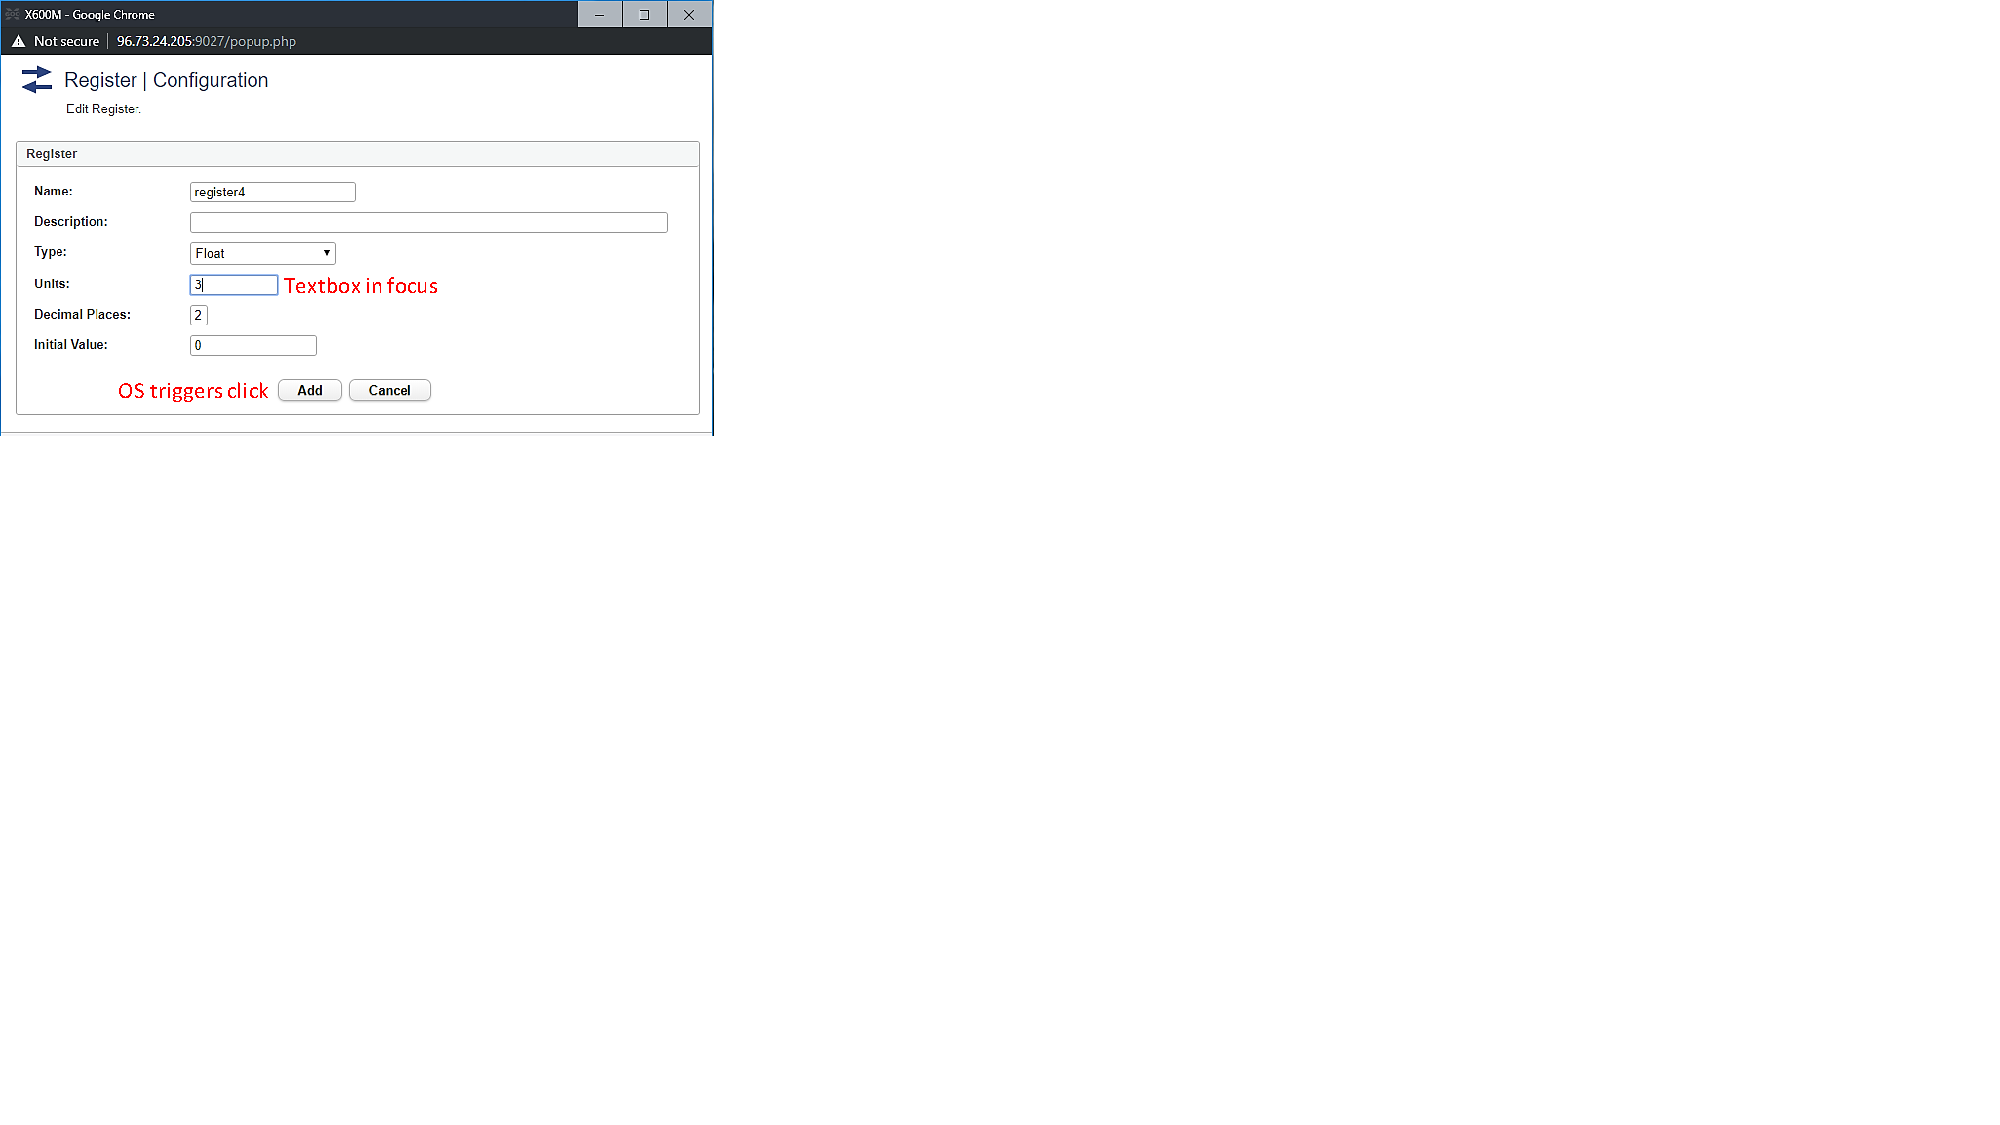
\includegraphics[trim={0 11.5cm 21.8cm 0}, clip, width=0.8\linewidth]{chapters/ProtectIOn/images/earlyFormSubmission.pdf}
\caption[Early form submission attacks]{\textbf{Early form submission attack} is possible on Fidelius~\cite{Fidelius}. The user selects and edits the field \emph{Units} while the OS triggers \emph{add} button, causing misconfiguration of a remote safety-critical PLC (Control by Web X-600M~\cite{controlbyweb}).}
\label{fig:clickJack}
\centering 
\end{figure}

Fidelius~\cite{Fidelius} addresses the problem with output integrity by rendering overlays using an external trusted device. Fidelius uses the trusted external device and Intel SGX to create a secure channel between the user IO devices and a remote server. The device intercepts user keystrokes and does not deliver any event to the untrusted host when the user types to secured text fields. Additionally, Fidelius renders an overlay with the user inputs on the screen, which is inaccessible by the host. This way, the untrusted host does not have access to raw inputs while the user sees them rendered on the screen as usual.
%provides secure input and display for the character-based device - keyboard. It uses overlays on the text fields to hide the keyboard input from the compromised host so that the input is only visible to the user. 
A small, trusted bar on display is also overlaid by the device that shows the remote server's identity and the text field that is currently selected. 
However, we observe a number of security and functional issues in Fidelius that we explain in the following. 

The overlay contains only the render of the user inputs into text fields, but the rest of the screen is rendered by the untrusted host.
This allows an attacker to modify the instructions on the UI, such as changing the input unit (typically described in the label of a text field) that could result in an incorrect input. This problem could be mitigated if the trusted bar includes the legitimate labels of the text fields also, although it would significantly increase the cognitive load to users.

%Fidelius solely relies on the static overlay bar and the LEDs on the external device to ensure the integrity and confidentiality of the input. 
Fidelius already introduces a high cognitive load to users as they need to monitor multiple security indicators simultaneously before filling up one text field. Previous research works~\cite{egelman2008you,sobey2008exploring, anderson2016warning} have shown that systems that require users to observe multiple security indicators %that require the users to observe multiple markers on the screen (and also on an external device) 
do not guarantee security in practice.
Also, in specific scenarios, even the training to properly explain these indicators to users could be a significant drawback for a real deployment.


\begin{mybox}[colback=white]{Observation 2}
If the \emph{protected output} is provided out-of-context, users are more likely not to verify it. Therefore input integrity can be violated.
\end{mybox}

%\noindent\emph{$\rightarrow$ Observation 2}: If the \emph{protected output} is provided out-of-context, users are more likely not to verify it. Therefore input integrity can be violated.


Fidelius does not consider the integrity of the mouse pointer and its interaction with UI elements, which broadens the attack surface. The lack of mouse support may appear to be a functional limitation, but it has non-trivial security issues.
The OS can arbitrarily trigger a mouse click on the submit button of a form while the user is typing and therefore send incomplete data to the server - early form submission attack.
This attack could cause the misconfiguration of a remote system, as illustrated in Figure~\ref{fig:clickJack}. Early form submission may appear to be similar to clickJacking attack, but the fundamental difference between them is that in clickjacking, the browser and OS are considered to be trusted. An untrusted OS can simply issue mouse clicks.

Moreover, Fidelius is also vulnerable to clickjacking attacks where the attacker can spawn a fake mouse pointer and trick the user into following it while the real mouse pointer is on a sensitive text field protected by the system. This allows the attacker to fool the user into providing (possibly incorrect) input while the user thinks that she is interacting with a non-sensitive text field. To prevent such attacks, the user has to look at the security indicators continuously even when she is not doing any security-sensitive task, which is a very strong assumption. 
Thus, not supporting the mouse causes the integrity violation of the keyboard input also.


\begin{mybox}[colback=white]{Observation 3}
If not \emph{all the modalities of inputs} are secured simultaneously, none of them can be fully secured.
\end{mybox}

%\noindent\emph{$\rightarrow$ Observation 3:} If not \emph{all the modalities of inputs} are secured simultaneously, none of them can be fully secured.


Finally, the design of Fidelius~\cite{Fidelius} is strictly limited to text-based fields only. As Fidelius does not provide output integrity of the forms, it cannot provide confidentiality to other UI elements such as radio buttons, drop-down menus, sliders, etc.
Microarchitectural attacks on Intel SGX~\cite{van2018foreshadow} increase the attack surface of the system significantly.


\myparagraph{B3. System TEE-based solutions} VButton~\cite{li2018vbutton} uses ARM TrustZone (TZ) to render UI buttons and receive user input from them securely. This is possible on mobile devices because the TZ architecture support flags on the system bus indicate whether an IO device like a touchscreen communicates with a trusted TZ application or the untrusted OS. Such solutions are infeasible for us because of the two following reasons. I) Secure communication between IO peripherals and TEE applications (like SGX enclaves) is not supported in the x86 architecture -- a similar system in x86 would require changes to the system architecture, TEE architecture, and IO devices. II) such solutions require TEE-aware applications and do not work with current browsers. Our goal is to design a solution that can be deployed on current x86 architecture and used with existing popular browsers.

\myparagraph{Strawman solution: Capturing screenshot} This strawman solution uses a trusted device that takes a screenshot when the user executes an action, e.g., mouse click to submit a form. The device then signs the snapshot and transmits it to the server along with the signed input. The remote server verifies the signature and then uses image/text analysis to extract the information from the UI elements such as labels on buttons or markers of a slider, etc. Therefore, the server would detect if the host has manipulated UI elements when presented to the user.

This method is vulnerable to attacks because it does not capture the spatio-temporal user context. This implies that the attacker may show some spatial information on the screen to influence the user that the snapshot may not capture. Furthermore, taking a full-screen snapshot could also reveal private information of the user from other applications. Similarly, taking a snapshot does not guarantee that a specific UI has been presented on the screen, as the attacker may render the legitimate UI shortly before the device captures the snapshot.
One way to mitigate this problem is to capture a video of user interaction. But such a method requires the host to send large amounts of data to the server, while the server should support video processing for different browsers, which is both time and CPU-intensive. Lastly, adversarial machine learning techniques~\cite{eykholt2017robust,sitawarin2018rogue} make the image/text recognition techniques insecure against advanced adversaries.


\subsection{Requirements of Security and Functional Properties}
\label{sec:problemStatement:goals}

We can summarize the above-discussed limitations of previous solutions as the following requirements for our solution:

\myparagraph{R1. Inter-dependency between input and output} 
The first and second observations from the existing solutions show that the output and input security depend on each other, and they should be considered together. Otherwise, the attacker can manipulate the output to influence the user input.

\myparagraph{R2. Inter-dependency between all input modalities} 
Existing web interfaces allow users to complete forms using different modalities for user input, namely the keyboard, the mouse, and the touchpad. The third observation shows that a secure system should simultaneously protect all user input modalities to achieve input integrity (against early-form submission and clickjacking).


\myparagraph{R3a. No cognitive load for IO integrity} 
A system that protects IO operations should introduce minimal or no cognitive load to its users for input integrity.
The system should guarantee the output integrity of the legitimate information necessary to complete a form and avoid asking the user to interact with an external device or monitor security indicators out-of-context.


\myparagraph{R3b. User attention for IO confidentiality} Preserving the confidentiality of user inputs against a compromised host is a challenging task because the host can trick the user into revealing her inputs when the system is not active. Therefore, requiring users to perform a small action, e.g., press a key before entering confidential inputs, is a valid tradeoff between usability and security.


\myparagraph{R4. Small trust assumptions and deployability} 
Our goal is to provide a rich set of IO and security features with minimal trust assumptions that do not rely on a trusted OS, specialized hypervisor, or TEEs such as Intel SGX. Preferably, the solution should be easy to set up for users, i.e., plug-and-play, and integrate well with the existing infrastructure.  

\section{Overview of Our Approach}
\label{sec:overview}


In this section, we provide an overview of our approach \name and introduce \emph{\nameenclave{}s}. \Nameenclave{}s dynamically extend the TCB of traditional TEEs running on the CPU to the \sphw. \Nameenclave{}s consist of multiple distributed enclaves that run on various hardware components such as the CPU and \sphw as shown in Figure~\ref{fig:new_system}. \Nameenclave{}s aim to provide similar security properties as traditional enclaves, such as integrity, attestation, and data isolation from other enclaves and the attacker-controlled OS. 

\begin{figure}[tbp]
    \centering
    %Source:
    %https://drive.google.com/file/d/1K8Jg0eXF1W2dpIVLmvP8D0k-qK-dHq4P/view?usp=sharing
    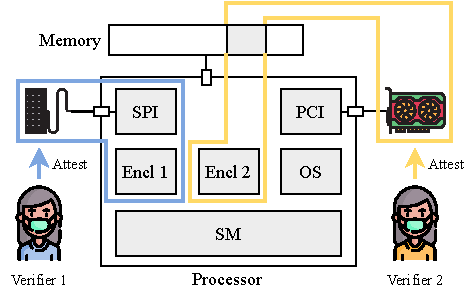
\includegraphics[width=0.7\linewidth]{chapters/PIE/images/cpu_bus_peripheral-Page-4.pdf}
        %   \includestandalone[width=\linewidth]{images/tikz/new_system}

    \caption[\Nameenclave{}s consists of different applications and \sphw]{Two \nameenclave{}s are highlighted by blue and yellow outlines. One consists of \texttt{Encl1} and the keyboard that is connected over the memory-mapped SPI bus. The second consists of \texttt{Encl2} and a GPU connected over PCI through DMA.}
    \label{fig:new_system}
\end{figure}



\subsection{Enclaves within a \nameenclave}
\label{sec:overview:enclaves}

A \nameenclave{} consists of multiple enclaves that run on different hardware components and securely communicate with each other. A \nameenclave{} typically contains several interconnected processor-local enclaves and \sphw enclaves. In the following, we describe the two main enclave types that form a \nameenclave{}.

\myparagraph{Processor-local enclaves}
\label{sec:overview:enclaves:processorEnclave}

Processor-local enclaves are equivalent to traditional enclaves and their runtime memory must be isolated from the OS and should only be accessible to the enclave itself. To achieve that, we use physical memory protection (PMP) from the RISC-V privilege standard~\cite{riscv2019privspec} as introduced by Keystone.

We further differentiate two types of processor-local enclaves: \app{}s, and \ce{}s which encapsulate the application-specific, and driver logic, respectively. As seen in Figure~\ref{fig:sharedMemory}, $AE_1$, and $CE_1$ are the \app, and \ce in the blue-outlined \nameenclave of Figure~\ref{fig:new_system}. The \ce also provides isolation between the \apps in a scenario where multiple \apps want to access a certain \sphw. Therefore, \ce enforces access control on the connected \apps in terms of how a certain \sphw can be accessed, e.g., exclusive access to a keyboard or shared concurrent access to a GPU. 
% $AE_1$ uses $CE_1$ to communicate with $P_1$ that is a \sphw enclave which we discuss in the following. 

\myparagraph{Enclaves on \sphw}
\label{sec:overview:enclaves:peripheralEnclave}
Most \sphw run some firmware or even some custom code (e.g., graphic shaders) which has to be included in the TCB of a \nameenclave.
E.g., the GPU and its firmware in Figure~\ref{fig:new_system} is part of the yellow \nameenclave. Since a remote verifier also wants to attest to the \sphw, they have to be modified to support attestation. However, we stress that these modifications  remain rather small (c.f. \Cref{sec:eval:accel}) and usually only involve small changes in the device firmware. %Essentially, one only has to add a certificate from the manufacturer for a secret key stored in the \sphw.

\begin{figure}[tbp]
     \centering
     %\includestandalone[width=0.9\linewidth]{images/tikz/approach}
     %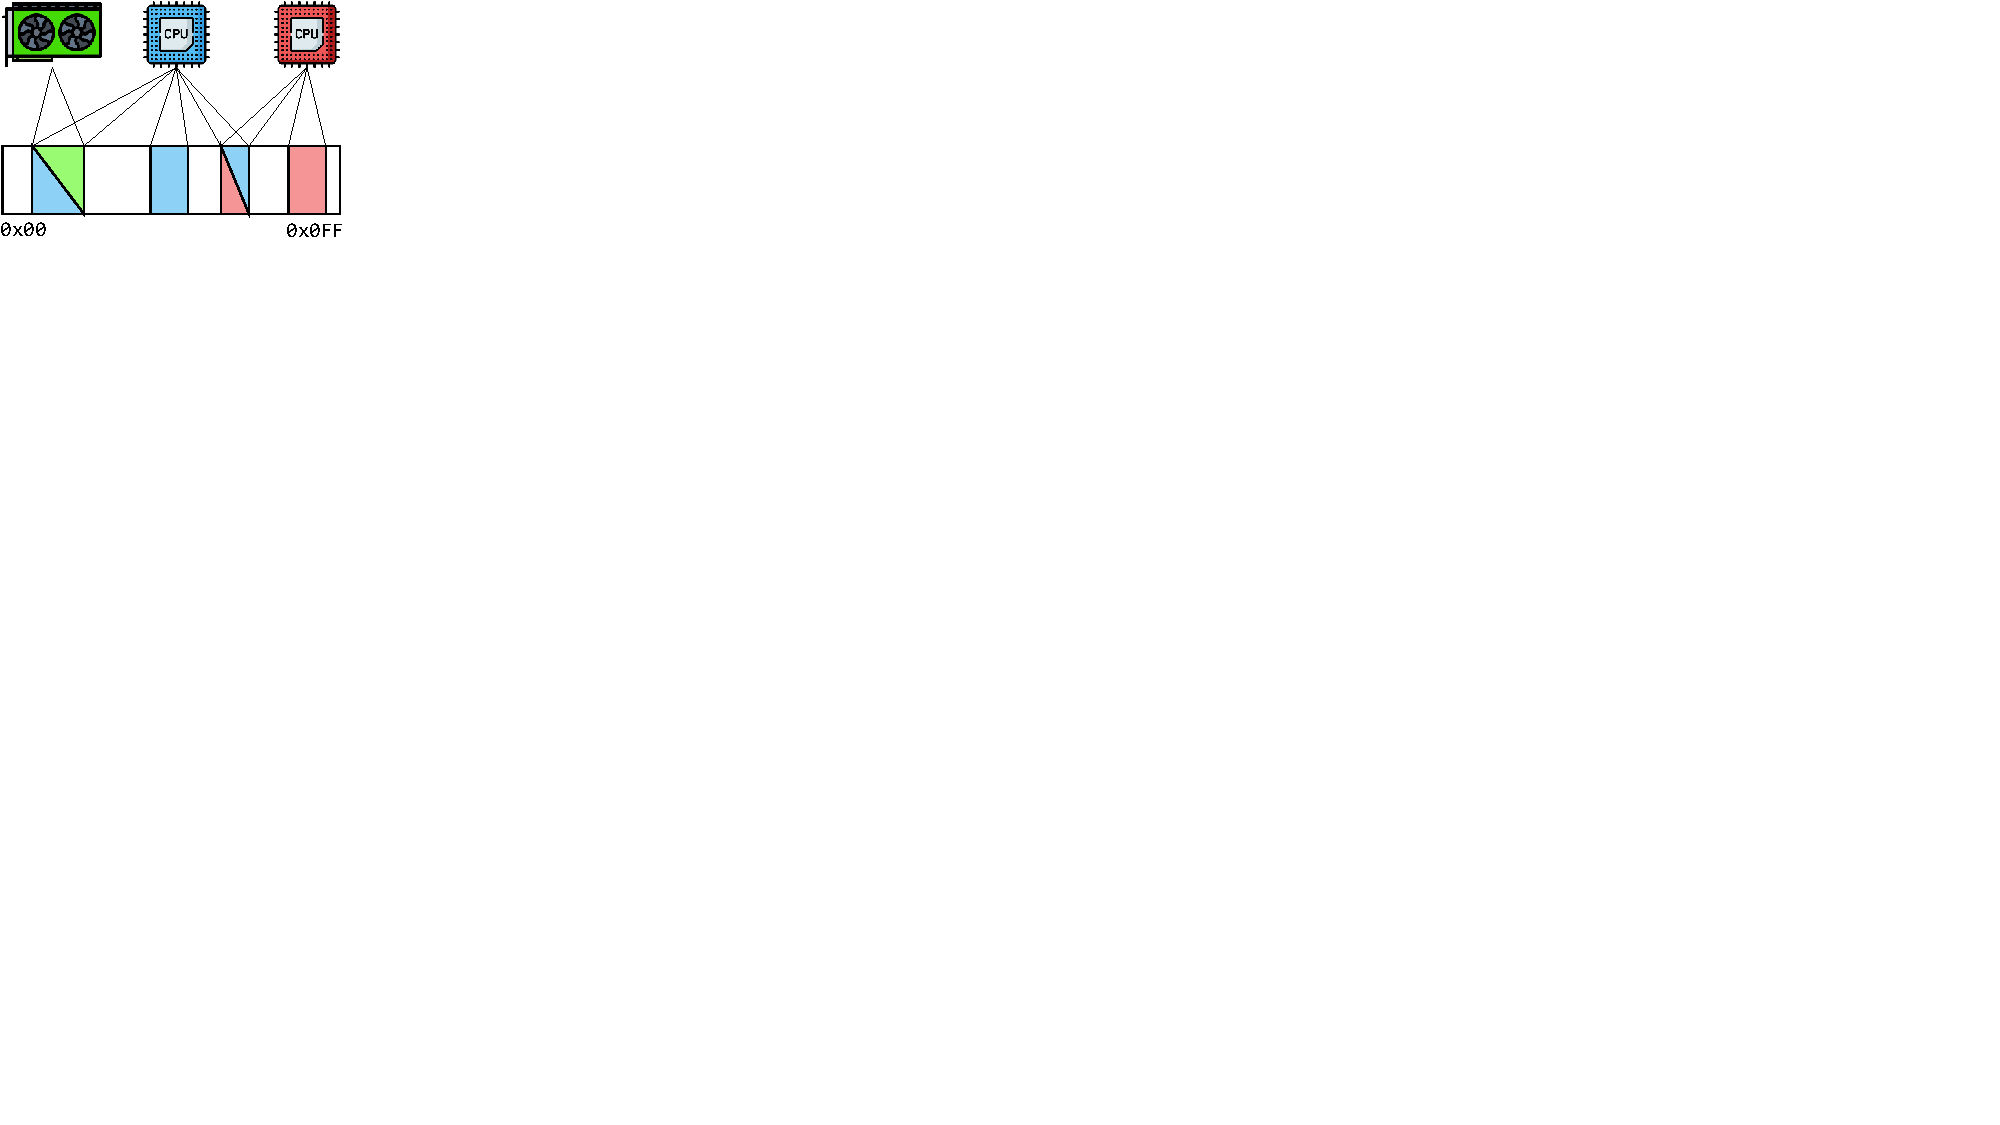
\includegraphics[trim={0 15cm 28cm 0}, clip, width=0.5\linewidth]{approach.pdf}
    %  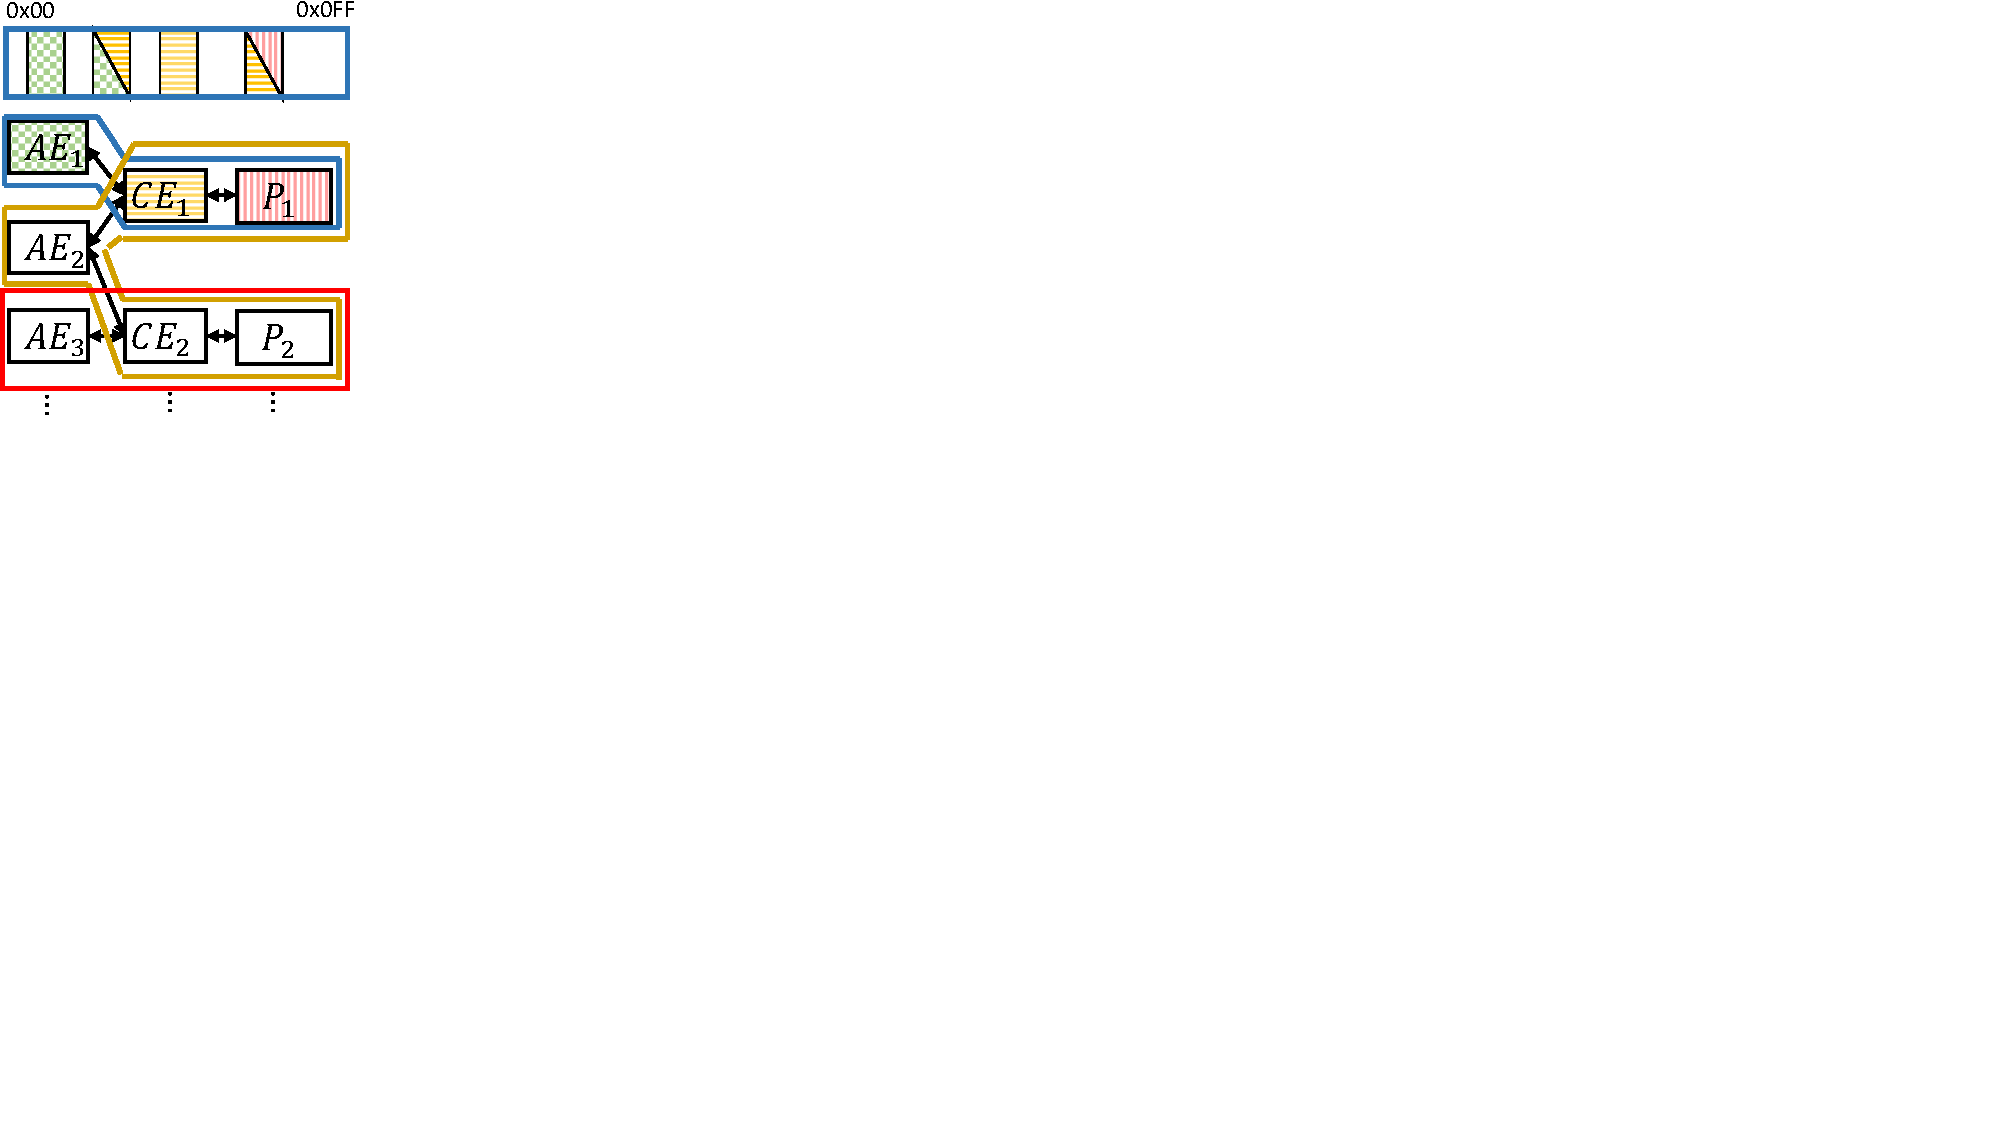
\includegraphics[trim={0 12cm 27cm 0}, clip, width=0.5\linewidth]{approach_combined.pdf}
     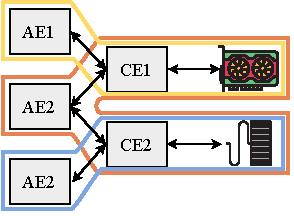
\includegraphics[width=0.4\linewidth]{chapters/PIE/images/softwaredesign.pdf}
     
     %\caption{Example configuration where a red CPU enclave shares some memory with a blue CPU enclave and another shared buffer with a GPU. The solid color memory cells correspond to the private enclave memory regions, and the cells with mixed color denote shared memory regions.}
     \caption[Three example \nameenclave{}s in \name{}'s software design]{Three example \nameenclave{}s in \name{}'s software design with \app{}s (AE), \ce{}s (CE), a GPU, and a keyboard. Note that the red \nameenclave{} is spanning over two external devices and \ce{}s isolate the data from the different \app{}s.}
     \label{fig:sharedMemory}
\end{figure}

\subsection{Communication with \sphw}
\label{sec:approach:comm}

To enable processor-local enclaves and \sphw enclaves to securely communicate, we make the observation that these devices generally communicate over mapped address regions: They either use an address range that is not reflected in DRAM, so-called memory-mapped-input-output registers (MMIO), or a shared DRAM region accessed via direct memory access (DMA). To maximize compatibility with existing drivers and \sphw, we chose not to change this behavior. Instead, we isolate the address regions that are used in this communication. Existing hardware mechanisms like PMP already allow restricting access to a specific address region. Until now, such hardware mechanisms have been predominantly used to restrict memory access, but in our design, they also allow to restrict access to other address regions that are not in the DRAM range\footnote{E.g., DRAM could occupy the address range \texttt{0x8000000 - 0xF0000000}, whereas other \sphw such as UART could reside at \texttt{0x4000000 - 0x4001000}.}. Note that these address regions from \sphw are either i) static, i.e., hardcoded and provided to the SM in the form of a trusted device tree file, or ii) dynamic, i.e., configured at runtime by the SM. In our design, the SM always maintains a complete overview of all such regions and only allows a single enclave to access an address region of a \sphw.

While we made the changes mentioned above to the SM to support \sphw with both MMIO and DMA, they also enable a new way for enclaves to communicate: shared memory. This reflects a major difference to traditional TEEs because until now; most traditional enclaves could only communicate through the untrusted OS\footnote{Concurrent work~\cite{yu2020elasticlave} has also shown how shared memory can improve the performance of enclaves significantly.}. 
% By supporting DMA regions for \sphw, our design also implicitly supports shared memory between enclaves. 
%Figure~\ref{fig:sharedMemory} shows an example shared memory configuration of our design.


\subsection{Changes within a \nameenclave{}}
\label{sec:overview:awareness}

The untrusted OS manages \sphw devices; hence the OS could remap any device or send a reset signal. E.g., a GPU that is handing sensitive data could be shut down by the OS and remapped to a different GPU during runtime. In such a scenario, the enclave should stop sending sensitive data to the GPU until the remote verifier re-attests the new GPU. Hence, the enclave has to react to these external events, i.e., it has to be aware of the platform's state. 
In traditional TEEs, enclaves are self-sufficient isolated entities and are only dependent on themselves. 
Therefore, they can only be in two states: running or stopped. \Nameenclave{}s are more complex since they can contain multiple enclaves, all of which could be running, stopped, or even killed. \Nameenclave{}s have to react correctly upon any of these events to keep the data confidential. We achieve this by expanding the enclave lifecycle and adding two new events: connect and disconnect. The asynchronous nature of these events requires a detailed analysis of the security of the entire system, e.g., a well-timed disconnect could lead to data leaks across shared memory regions. We solve this issue by assigning ownership of the shared memory among the enclaves that are accessing that memory. Upon any external events, if one of the participating enclaves dies, the sole ownership is transferred to the remaining one (more details in \Cref{sec:lifeycle}). Therefore, the components in the \nameenclave are \emph{platform-aware} since they are aware of any change within their ecosystem.


\subsection{Attestation of a \nameenclave{}}

Since a \nameenclave{} consists of multiple distributed enclaves, attestation poses another challenge. Individual attestations to each enclave that make up a \nameenclave{} could be vulnerable to timely manipulations by an adversary to cause time-of-check-to-time-of-use (TOCTOU) issues. To provide a platform-wide attestation, we need to chain attestation reports of all the components of a \nameenclave. This includes the attestation report of the enclaves and \sphw firmware. Attestation of the \sphw firmware is achieved by signing a challenge message with the key embedded in the \sphw (refer to Section~\ref{sec:overview:enclaves:peripheralEnclave}).
The attestation of a \nameenclave{} could either be a one-time attestation that results in a huge chain of reports or individual attestations of all entities that can be combined by the verifier. 
We show that individual attestations provide more flexibility for the verifier and are secure against TOCTOU attacks by adding unique identifiers to enclaves and appending all connected enclaves' IDs to the attestation report.
%% Ivan: I have removed the following cause it adds no value to the discussion at this point 
%Surprisingly, this even remains true when identifiers are reused. 


% The full state of a system is too detailed to be processed every time it changes or to meaningfully assess whether it is safe for a remote stakeholder to provide its data. Therefore, this last challenge requires concretely defining what parts of the state (and state transitions) of a system are relevant for the security of \name{}.

\begin{figure}[tbp]
    \centering
    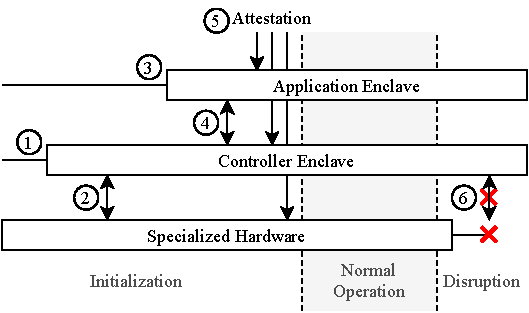
\includegraphics[width=0.8\linewidth]{chapters/PIE/images/cpu_bus_peripheral-Page-5.pdf}
    \caption[Interactions between \nameenclave's components]{An example scenario that illustrates interaction between \nameenclave components.}
    \label{fig:overviewtime}
    % \vspace{-1em}
\end{figure}

\subsection{Summary of Interactions}
To summarize all interactions between the components of a \nameenclave, we present an example scenario in Figure~\ref{fig:overviewtime} with an \app{}, a \ce{}, and a \sphw device. The scenario is as the following:
\begin{enumerate}
    \item[\one] The OS creates and configures the \ce{} and hands over control to the SM. The SM then revokes the OS's access permissions to the private memory regions of the \ce{}.
    \item[\two] The OS requests SM to connect \ce{} with the \sphw device. The SM sets up a new shared memory region and enables access only to the \ce{}.
    \item[\three] Similar to the \ce, the OS creates and configures the \app{}, and then, once again, the SM revokes access to the private memory of the enclave.
    \item[\four] The OS calls the SM to establish a shared memory region between the \ce and the \app. 
    \item[\five] After a remote verifier attests to all enclaves (using the \app as the entry point), sensitive data can be transmitted, and the normal operation starts.
    \item[\six] Any disruption, i.e., a disconnection of the \sphw device, leads to an asynchronous disconnect, where the sole ownership of the shared memory between the device and the \ce{} moves to \ce(see Section~\ref{sec:lifeycle}). Moreover, the enclaves may halt execution until re-attested.
\end{enumerate}

% \subsection{Software Design}

% The last major challenge is to make \name easy to adapt for existing software and \sphw (refer to challenge \emph{d} in Section~\ref{sec:problemStatement:challenges}). A \nameenclave{} must include the driver for any \sphw that it wants to use. However, one big monolithic processor-local enclave that contains all drivers has many downsides. First, \sphw are fully reserved by a single processor-local enclave and cannot be shared among multiple enclaves. And second, every other enclave that also wants to use the same \sphw must also include a driver leading to massive code duplication or, even worse, multiple driver implementations for the same \sphw, each with their own vulnerabilities.

% To combat these downsides of a big monolithic processor-local enclave, we propose a modular software design. All the application logic is kept in an enclave that we call \app. And the driver for a single \sphw is moved to an enclave called \ce{}. This allows multiple \app to use the same \sphw and driver concurrently over one \ce{}. However, to enforce the confidentiality of the various enclaves' data, the \ce{} has to isolate the data, adding to the TCB. This design choice reflects a trade-off between code reuse and usability, and a bit of added complexity and TCB. Note that such a software design also has a significant impact on the attestation mechanism. To remotely attest a \nameenclave{}, the user must attest the \app, all the \ce{}s that it is connected to, and all the \sphw that the \ce{}s are accessing.

\section{Platform Isolation Environment}
\label{sec:approach}

In this section, we describe Platform Isolation Environment or \name in detail. \name is based on the idea of \nameenclave{}s that integrates \sphw devices to the traditional processor-core enclaves while maintaining small hardware and software TCB. First, we discuss the changes needed to incorporate into the \sphw to make them compatible with \name. Then we introduce a shared memory model that allows enclaves to communicate with each other and \sphw securely. Next, we discuss how the enclave life cycle changes given these modifications and how a remote verifier can get proof of the state of a \nameenclave{}. Finally, we provide a software design for \name that makes \name for the software developers easy to adapt.


 \begin{figure}[t]
     \centering
     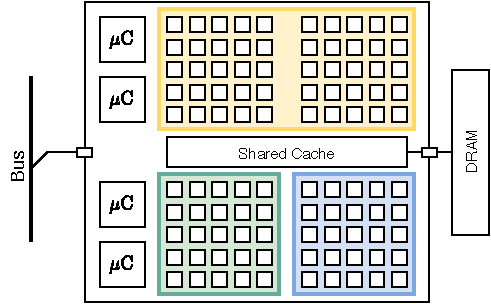
\includegraphics[width=0.8\linewidth]{chapters/PIE/images/accelerator.pdf}
     \caption[Example of a TEE on an accelerator with multiple enclaves running simultaneously while being isolated from each other]{\textbf{Example of a TEE on an accelerator} with multiple enclaves running simultaneously while being isolated from each other. In this example, there are three distinct enclaves running on a subset of the compute units of the accelerator indicated by a yellow, green, and blue overlay.}
     \label{fig:accelerator}
 \end{figure}

\subsection{Changes to \sphw} There exists a wide range of \sphw{} devices that have unique behavior and integrate differently into \name{}.  In this chapter, we try to cover most devices but stress that some special cases require further analysis. We go from the simplest \sphw device we can imagine, a simple sensor, to one of the most complex, a sophisticated accelerator for a data center. Most other \sphw devices should fall in between these two examples and thus may require modifications between these two extremes. 

\begin{enumerate}
\item\emph{Sensors and IO peripherals} e.g., a temperature sensor only requires a minimal form of attestation to be integrated into \name{}. They must contain some key materials to sign some statements about themselves. This is mandatory for (remote) attestation of a \nameenclave that includes an attestation report of such a sensor. Usually, these sensors do not contain any secret data from a processor-local enclave and hence do not need to protect such data.

\item\emph{Accelerators} on the other hand, tend to be very complex and require more extensive modifications. Like the former, they must support attestation, but they may also support isolation for multiple enclaves' secret data. Let us assume data-center applications, where multiple stakeholders want to move multiple compute-intensive tasks from the CPU to the accelerator. The individual tasks' data should remain confidential and isolated, not only on the CPU but also on the accelerator (as seen in Figure~\ref{fig:accelerator}). Thus, such an accelerator requires isolated and attestable domains -- in other words -- enclaves that run on the \sphw. 

\end{enumerate}

\subsection{Shared memory}
\label{sec:approach:sharedMemory}
Shared memory is a common mechanism for software to communicate across multiple cores or DMA regions of a \sphw. In our prototype, shared memory regions are centrally maintained by the CPU to enforce isolation as all \sphw is connected to the CPU.


\begin{enumerate}
\item\emph{Shared Memory between Processor-local Enclaves}
As mentioned before, processor-local enclaves rely on PMP entries for isolation. We reuse the functionality of PMPs also to protect shared memory regions. Therefore, our proposal does not require any changes to the processor itself, as PMP is already part of the RISC-V standard~\cite{riscv2019privspec}, and thus, it is already part of many processors. The SM, however, requires some modifications. For example, to store the configuration details for every shared memory region in local memory, the SM needs to reconfigure the PMP entries on a context switch similar to stock Keystone. It also must guarantee that at most two entities have access to the same shared buffer at a time. Additionally, the SM flushes the buffers' content when one enclave is destroyed not to leak stale data. 


\item\emph{Shared Memory with \sphw} \Sphw are connected to the CPU over buses, which are, in turn, controlled by bus controllers. As mentioned in \Cref{sec:overview}, \sphw communicate over memory-mapped address ranges either in the form of MMIO registers or DMA memory regions. To isolate these address regions, we rely on existing hardware mechanisms, mainly PMP. Until now, such hardware mechanisms have predominantly been used to restrict memory access, but they can also be used to restrict access to any other address that is not in the DRAM range. Our prototype reuses the concepts from shared memory between processor-local enclaves by assuming the \sphw to be another processor-local enclave. As such, it can directly share an address range with a real processor-local enclave. The SM represents a \sphw internally as a special case of a processor-local enclave that cannot be scheduled or called, but it may share some address regions with other enclaves. 

\end{enumerate}

% \begin{figure}[tbp]
%     \centering
%      \includestandalone[width=\linewidth]{images/tikz/lifecycle}
%     \caption{\textbf{The lifecycle of platform-wide enclaves.} The differences to traditional enclaves is highlighted in green. Note that, asynchronous disconnects can happen in all three possible states.\moritz{todo: beautify, or maybe change completely}}
%     \label{fig:lifecycle}
% \end{figure}


% \begin{figure}[t]
%   \centering
%   %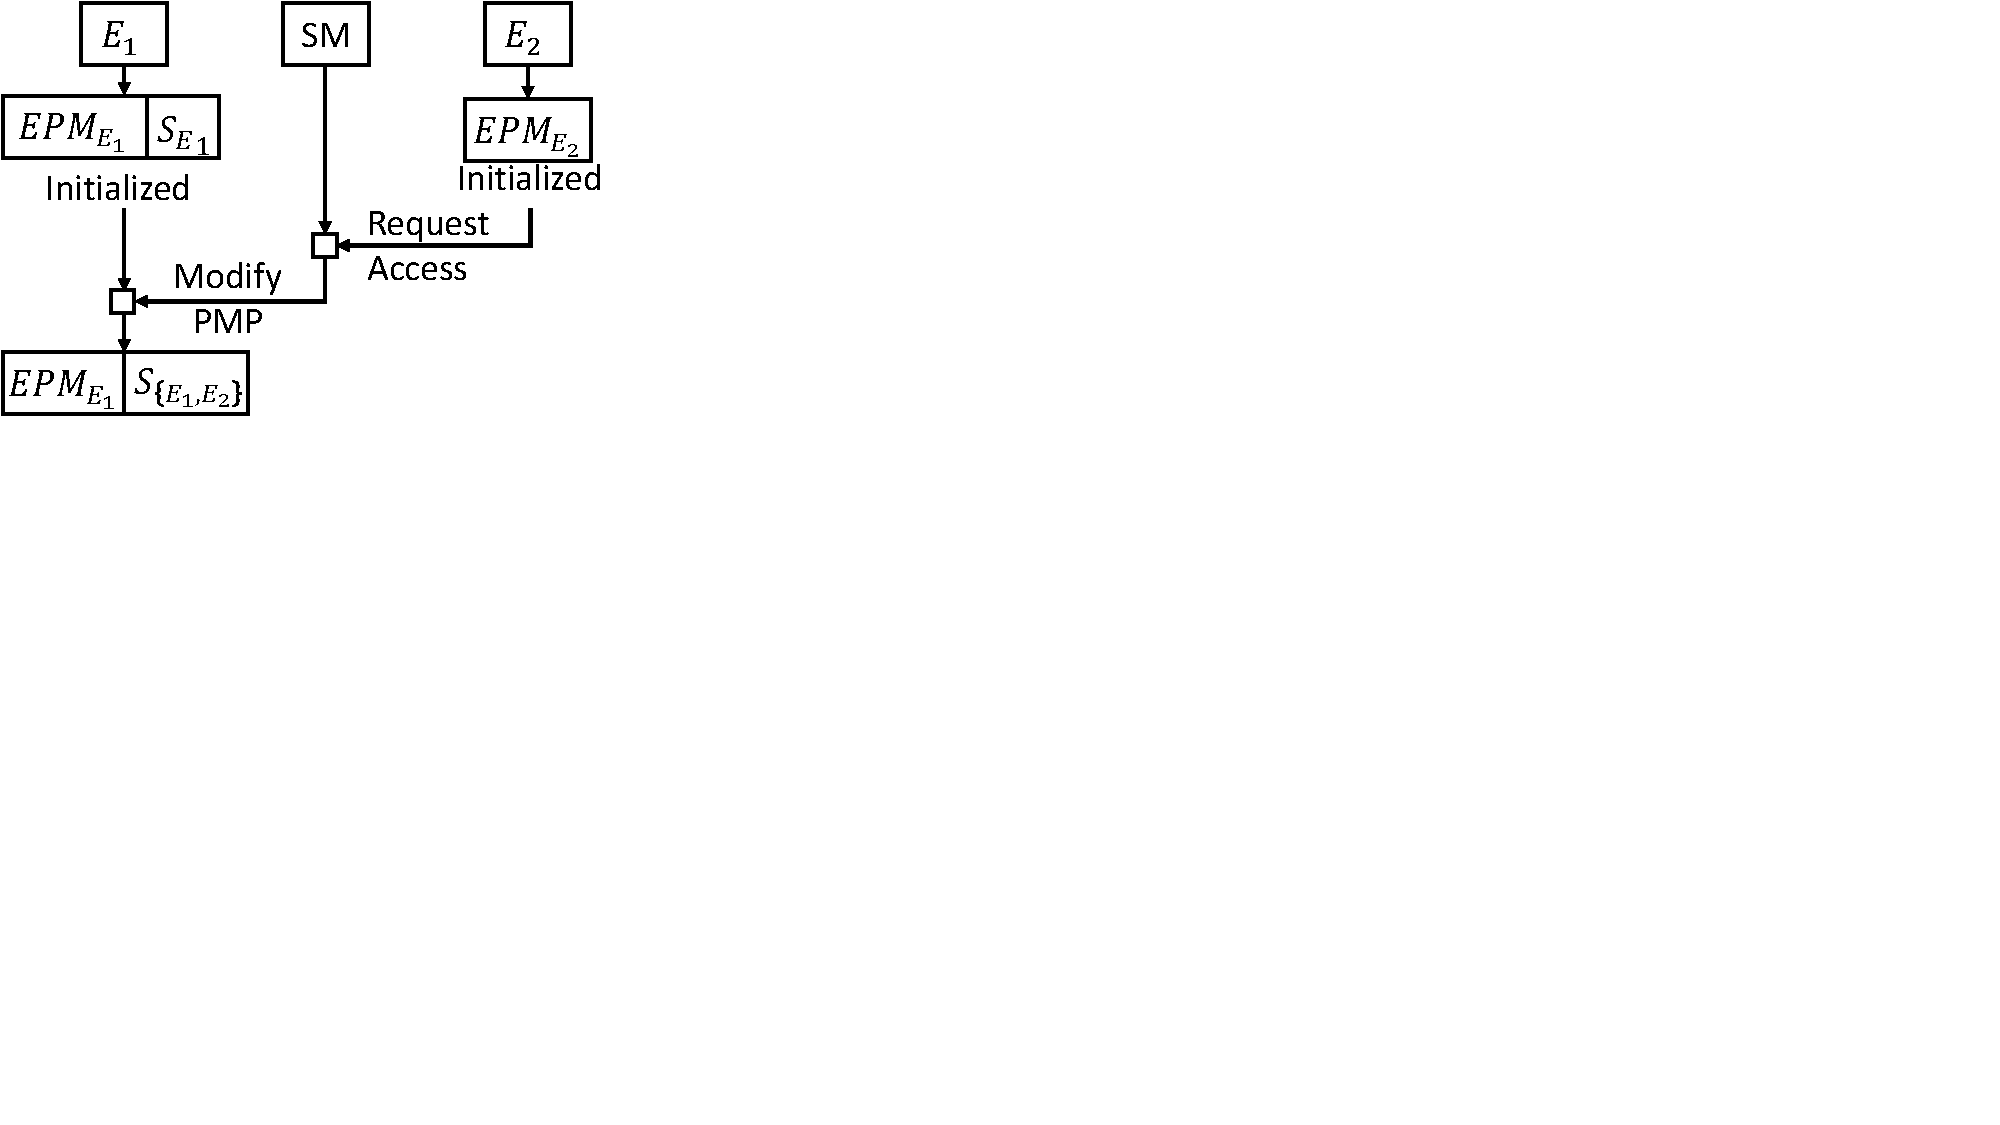
\includegraphics[trim={0 12cm 23cm 0}, clip, width=0.65\linewidth]{sharedMemoryInit.pdf}
%   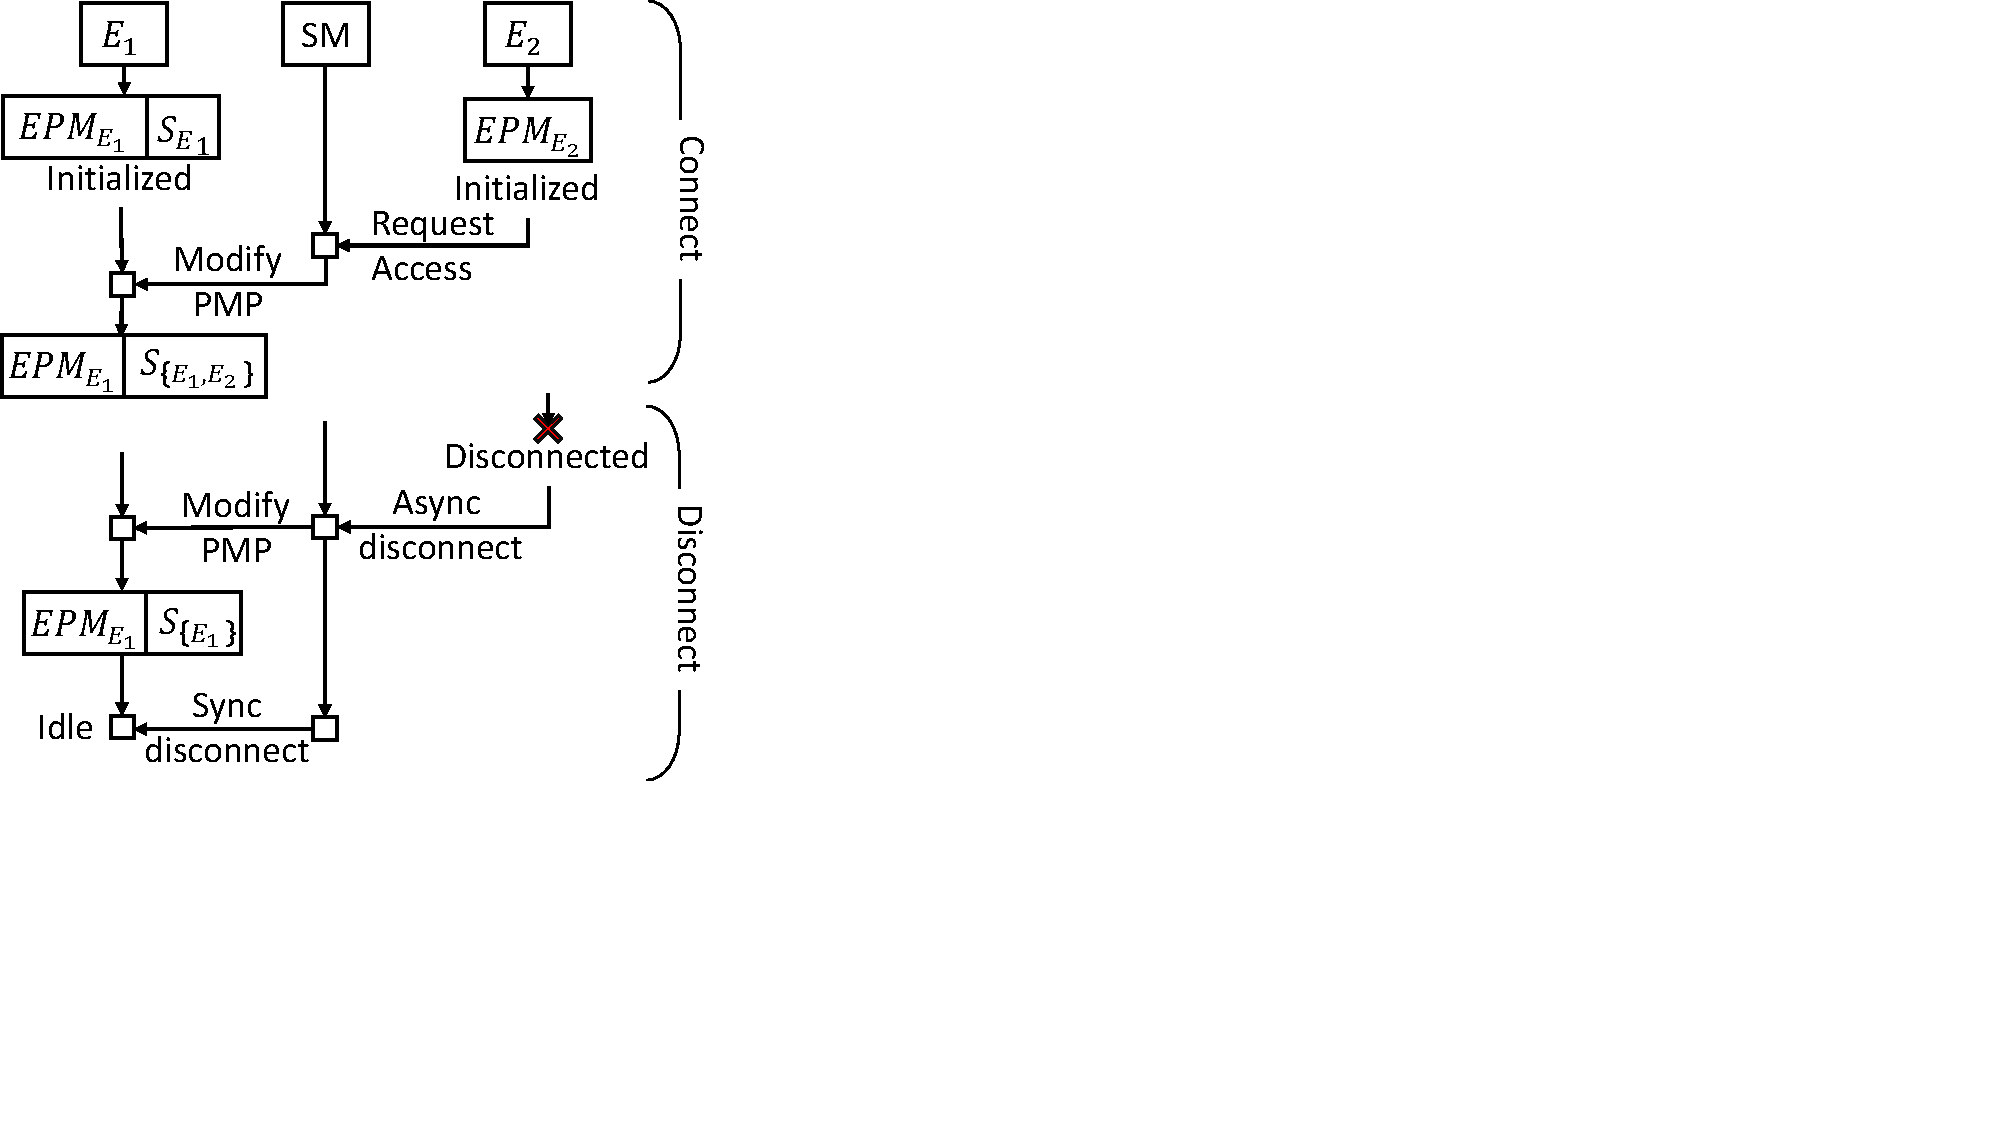
\includegraphics[trim={0 5.4cm 22cm 0}, clip, width=0.65\linewidth]{lifeCycle.pdf}
%   \vspace{-1em}
%   \caption{The life-cycle events of two example enclaves $E_1$ and $E_2$. $EPM_{E_1}$ and $EPM_{E_2}$ denote the enclave private memory (EPM) regions of $E_1$ and $E_2$ respectively. $S$ stands for the shared memory region and the subscript denotes the enclave(s) it is shared between. The security monitor (SM) acts as the intermediary in the \texttt{connect} and \texttt{disconnect} events.} \vspace{-1.2em}
%   \label{fig:sharedmemexample}
% \end{figure}

\myparagraph{Polling and Interrupts}
\sphw are synchronized with the processor with either polling or interrupts. Polling requires the CPU to check at a predetermined rate if new data is available from the \sphw, and thus, it can immediately be used in \name{}. On the other hand, interrupts are more complicated as they enable the \sphw to notify the CPU that new data is available with the processor's hardware support. In RISC-V specifically, interrupts can be delegated from the highest privilege mode to lower ones. So, in our prototype of \name{}, the SM can delegate individual types of interrupts either to an enclave or to the OS\footnote{In RISC-V external interrupts are handled by the platform interrupt controller (PLIC) and then multiplexed on top of the external interrupt signals to the core. Thus the SM has to contain a driver for the PLIC to figure out which \sphw the interrupt is from.}. Therefore, enclaves could also contain interrupt-handlers to, e.g., handle interrupts for a specific \sphw. Note that in our prototype, we only focus on polling. 

\subsection{Enclave life cycle}
\label{sec:lifeycle}

Traditional enclave's life cycle includes three distinct states: idle, running, and paused. E.g., the enclave is first created and started in the idle state. Then the enclave transitions to the running state after a call from a user. Due to a timer interrupt by the OS scheduler, it is paused. It resumed again as soon as the scheduler yields back to the enclave. 

\myparagraph{Attaching \sphw}
Before going into the lifecycle details, it is crucial to understand how \sphw are \emph{attached} to the platform and initialized.
There are two types of initialization procedures: statically compiled in the device tree or dynamically mapped by a bus controller. 
The device tree describes the specific address ranges and model numbers of all statically connected \sphw devices. It is usually stored in on-chip ROM and is provided to the OS by a zero-stage boot-loader, and thus, it can be considered trusted.
Dynamically mapped devices are mapped by a bus controller and a driver to a DMA region. In our proposal, the bus controller's driver, which sets up the DMA region, has to be trusted.

\myparagraph{Changes during runtime}
In \name{}, we introduce two additional life cycle events to describe what happens when a shared memory region is altered. These are \emph{connect} and \emph{disconnect} that are needed due to the asynchronous nature of \sphw as they can prompt a disconnect event at any time.

The asynchronous disconnects are very critical as an enclave could end up continuing to use a memory region that is no longer protected due to a disconnect. Additionally, enclaves might want to provide graceful degradation and should not crash completely upon a disconnect. We solve both issues by splitting the disconnect event into an asynchronous disconnect and a synchronous disconnect. We consider both enclaves or \sphw of a shared memory region to have shared ownership over that region. If one of the entities dies, the other entity gains the sole ownership of the memory region. As such, an asynchronous disconnect leads to the sole ownership of a previously shared memory region. In turn, the untrusted OS can issue a synchronous disconnect command to the SM to free the shared memory region and notify the enclave of the disconnect. We mandate that before any connect command, the enclave must first receive a synchronous disconnect. If this was not the case, an attacker could disconnect a benign \sphw and reconnect a malicious one without the enclave noticing.


We illustrate the behavior of a \nameenclave{} in various circumstances using an example scenario. \emph{enclave 1} ($E_1$) connected to \emph{enclave 2} ($E_2$). $E_2$ then is connected to a \sphw ($HW$). We denote the shared memory spaces as $S_{\{E_1, E_2\}}$, and $S_{\{E_1, HW\}}$that is shared among $E_1$ \& $E_2$, and $E_1$ \& $HW$ respectively.

\begin{enumerate}

\item\emph{$E_1$ is killed.} In such a situation, the specific shared memory space $S_{\{E_1, E_2\}}$ should be destroyed. To do that, the SM performs an asynchronous disconnect of $E_2$ for $S_{\{E_1, E_2\}}$ resulting in sole ownership of $S_{\{E_1, E_2\}}$ by $E_2$. Upon the following synchronous disconnect $S_{\{E_1, E_2\}}$ gets fully destroyed.

A specific application may require any sensitive data from $E_1$ that is still on $HW$ to be cleared. In such a scenario, $E_2$ will tell $HW$ to clear this data on the following synchronous disconnect. Note that how the \sphw handles this call is also dependent on the implementation of that \sphw firmware enclave. For example, a \sphw that handles sensitive user data may decide to terminate the session completely (by zeroing out all the internal states) and destroy the shared memory between the \sphw and $E_2$.

    
\item\emph{$E_2$ is killed.} All shared memory regions associated with $E_2$ (this includes the shared memory spaces with both $E_1$ and $HW$) are immediately modified by the SM during the asynchronous disconnect. They are now solely owned by $E_1$ and $HW$, respectively. Zeroing out $S_{\{E_2, HW\}}$ also implicitly notifies $HW$ that $E_2$ has died, forcing the \sphw to reset.
    
\item\emph{$HW$ is killed/disconnected} In the asynchronous disconnect, the SM immediately modifies $S_{\{E_2, HW\}}$ to $S_{\{E_2\}}$. At some later point, the OS must issue a synchronous disconnect, which invalidates $S_{\{E_2\}}$. This also results in the destruction of $S_{\{E_1, E_2\}}$ in case $E_1$ accesses $HW$ through $E_2$. From then on $E_2$ is available to connect to a new $HW$ (after attestation).

\end{enumerate}

\subsection{Attestation of a \nameenclave{}}
\label{sec:approach:attestation}

We extend the existing notion of attestation from processor-local enclaves to \nameenclave{}s that run on multiple components of the platform. Traditionally, attestation ensures the current state of an enclave through a measurement of the code. The standard attestation report of a traditional enclave contains the measurements of both enclaves and the low-level firmware (e.g., the security monitor in RISC-V keystone). Both of which are signed by the platform key (known as the device root key). In contrast, an attestation of a \nameenclave{} must also reflect all included components. 
A potential attestation mechanism for a \nameenclave{} would be a lengthy report containing all the components' measurements. %However, for very 
Contrary to that, we provide the verifier with an option to decide which other enclaves he wants to attest. When the verifier attests a specific component of a \nameenclave, a list of identifiers of all the connected components is provided alongside the attestation report. These identifiers are assigned by the SM on the processor and can be used to specify which enclave one wants to attest. A verifier can then chose to attest some or all the connected enclaves from the list of identifiers if he wishes to do so.


\myparagraph{Enclave identifiers} 
Upon creation of a new processor-local enclave, SM assigns a unique identifier to it. This identifier uniquely determines the enclaves participating in a specific shared memory region. When the enclave is killed, the identifier may be reused for other enclaves (refer to~\Cref{sec:securityAnalysis}).


% \subsubsection{Attestation Process between Programming Model Components}
% \label{sec:programmingModel:attestation:process}
\begin{figure}[t]
  \centering
  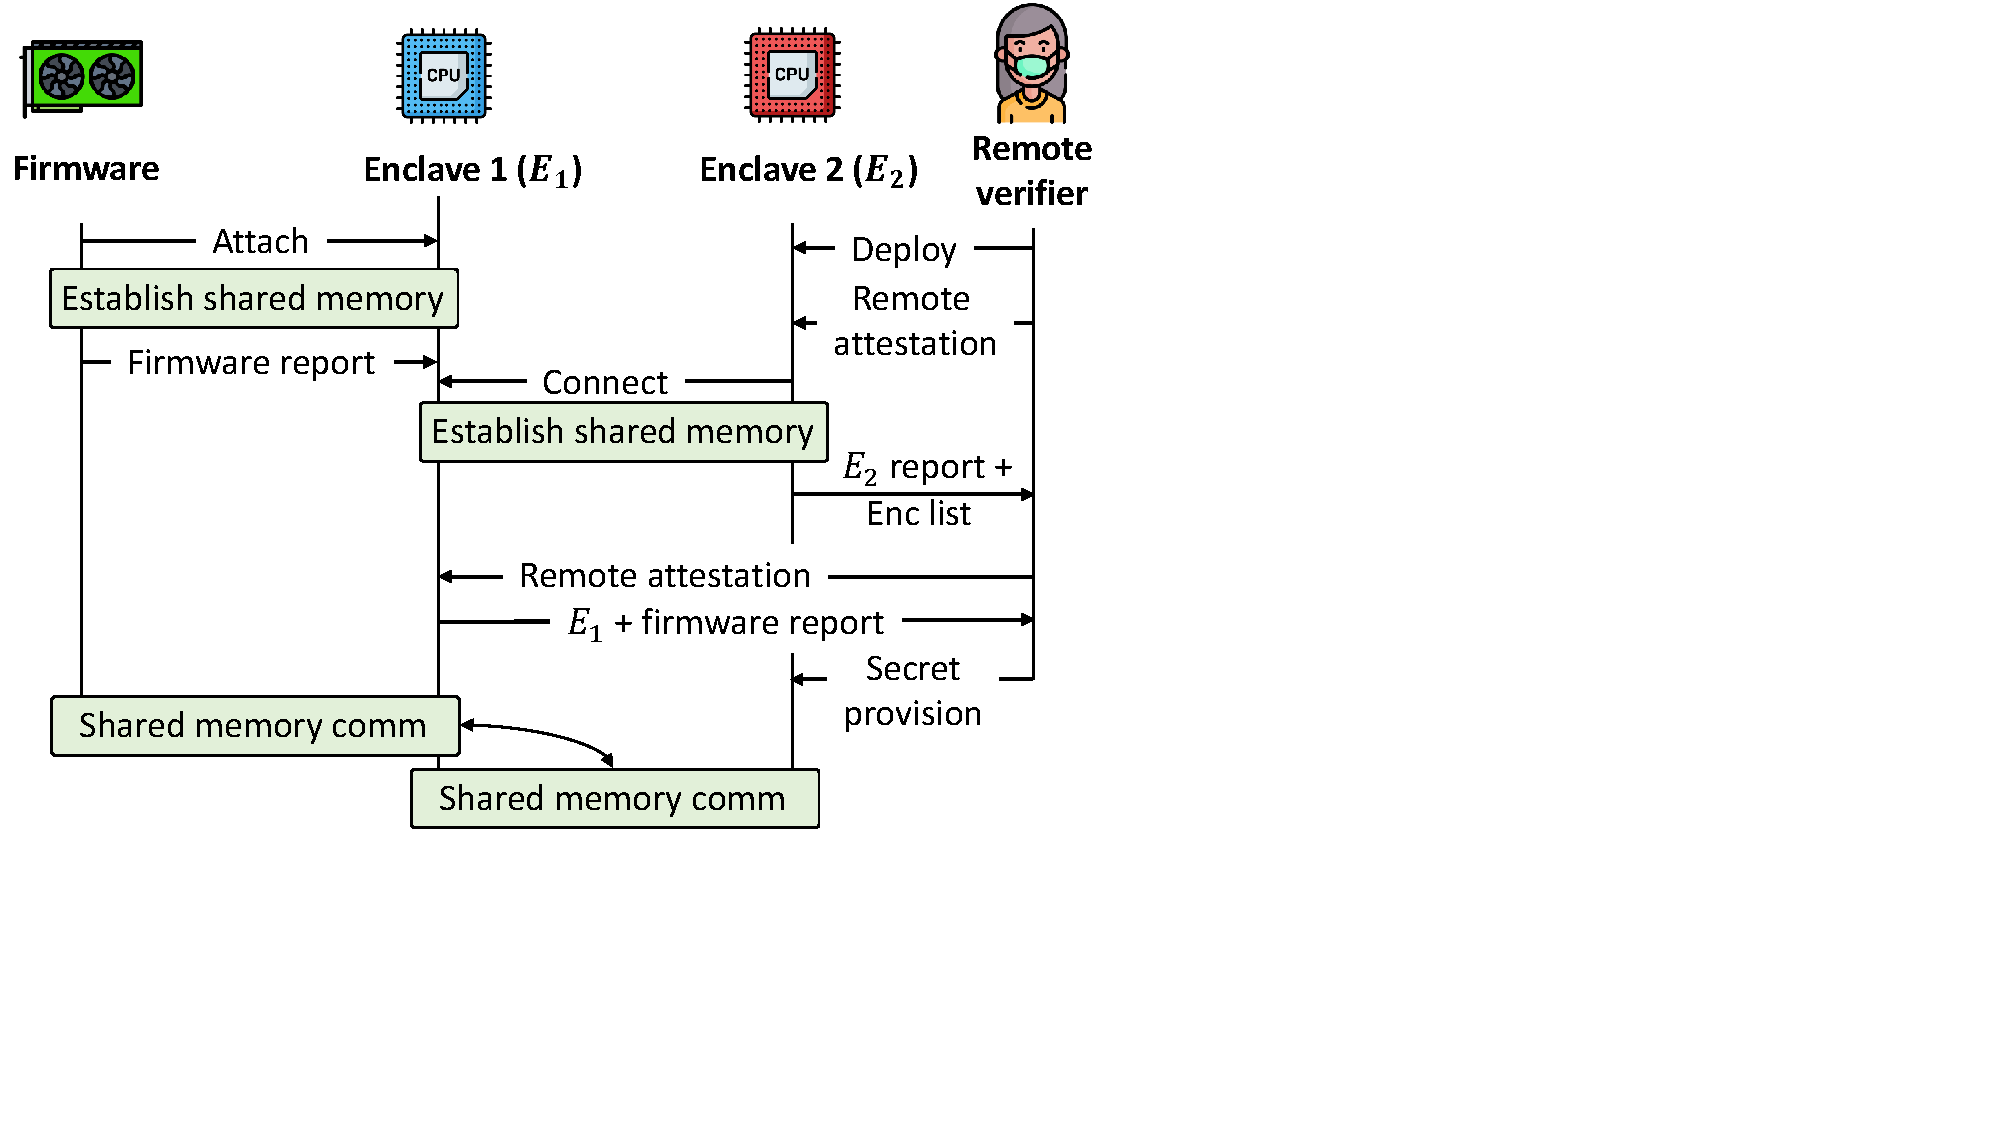
\includegraphics[trim={0 5cm 15cm 0}, clip, width=.8\linewidth]{chapters/PIE/images/localAttestation.pdf}
  \caption[Flow of (remote) platform-wide attestation process between \nameenclave{}'s components]{\textbf{Flow of the (remote) platform-wide attestation process} between the remote verifier, $E_1$, $E_2$ and the \sphw firmware. At the end of this process, the remote verifier receives the attestation report of $E_1$, $E_2$, and \sphw firmware, including their connection parameters such as DMA size, peripheral access control policy, etc.}   
  \label{fig:attestationFlow}
\end{figure}

\myparagraph{Attestation Flow}

Figure~\ref{fig:attestationFlow} depicts an example \nameenclave{} and the sequence of the attestations between its different components.The \name enclave contains three components \emph{enclave 1} ($E_1$), \emph{enclave 2} ($E_2$) and a \sphw firmware. Note that the platform-wide attestation process starts from the verifier who initiates a remote attestation request of $E_2$. 
The attestation report of $E_2$ includes a list  of connected enclaves' identifiers, notably $E_1$. The verifier then executes a series of individual remote attestations of all connected enclaves. Note that both individual attestations of $E_1$ and $E_2$ include each other's identifier in their list of connected components. Note that both the attestation reports of $E_1$ and $E_2$ are signed by the same platform key. This proves to the remote verifier that both the enclaves are running on the same platform.

For \sphw, the attestation mechanism is different. First of all, a \sphw needs to contain some key material and a signed certificate from the manufacturer. This allows a verifier to observe the legitimacy of the \sphw. Secondly, the verifier from \Cref{fig:attestationFlow} needs to be able to verify that the \sphw is directly talking to $E_1$. This is facilitated by the SM, who checks the address regions for MMIO registers. DMA regions can even be established by an untrusted entity such as the OS. However, the attestation report of both the \sphw and $E_1$ contains the physical memory region that they share.


% \input{sections/ourApproach}
% \begin{figure*}[t]
\centering
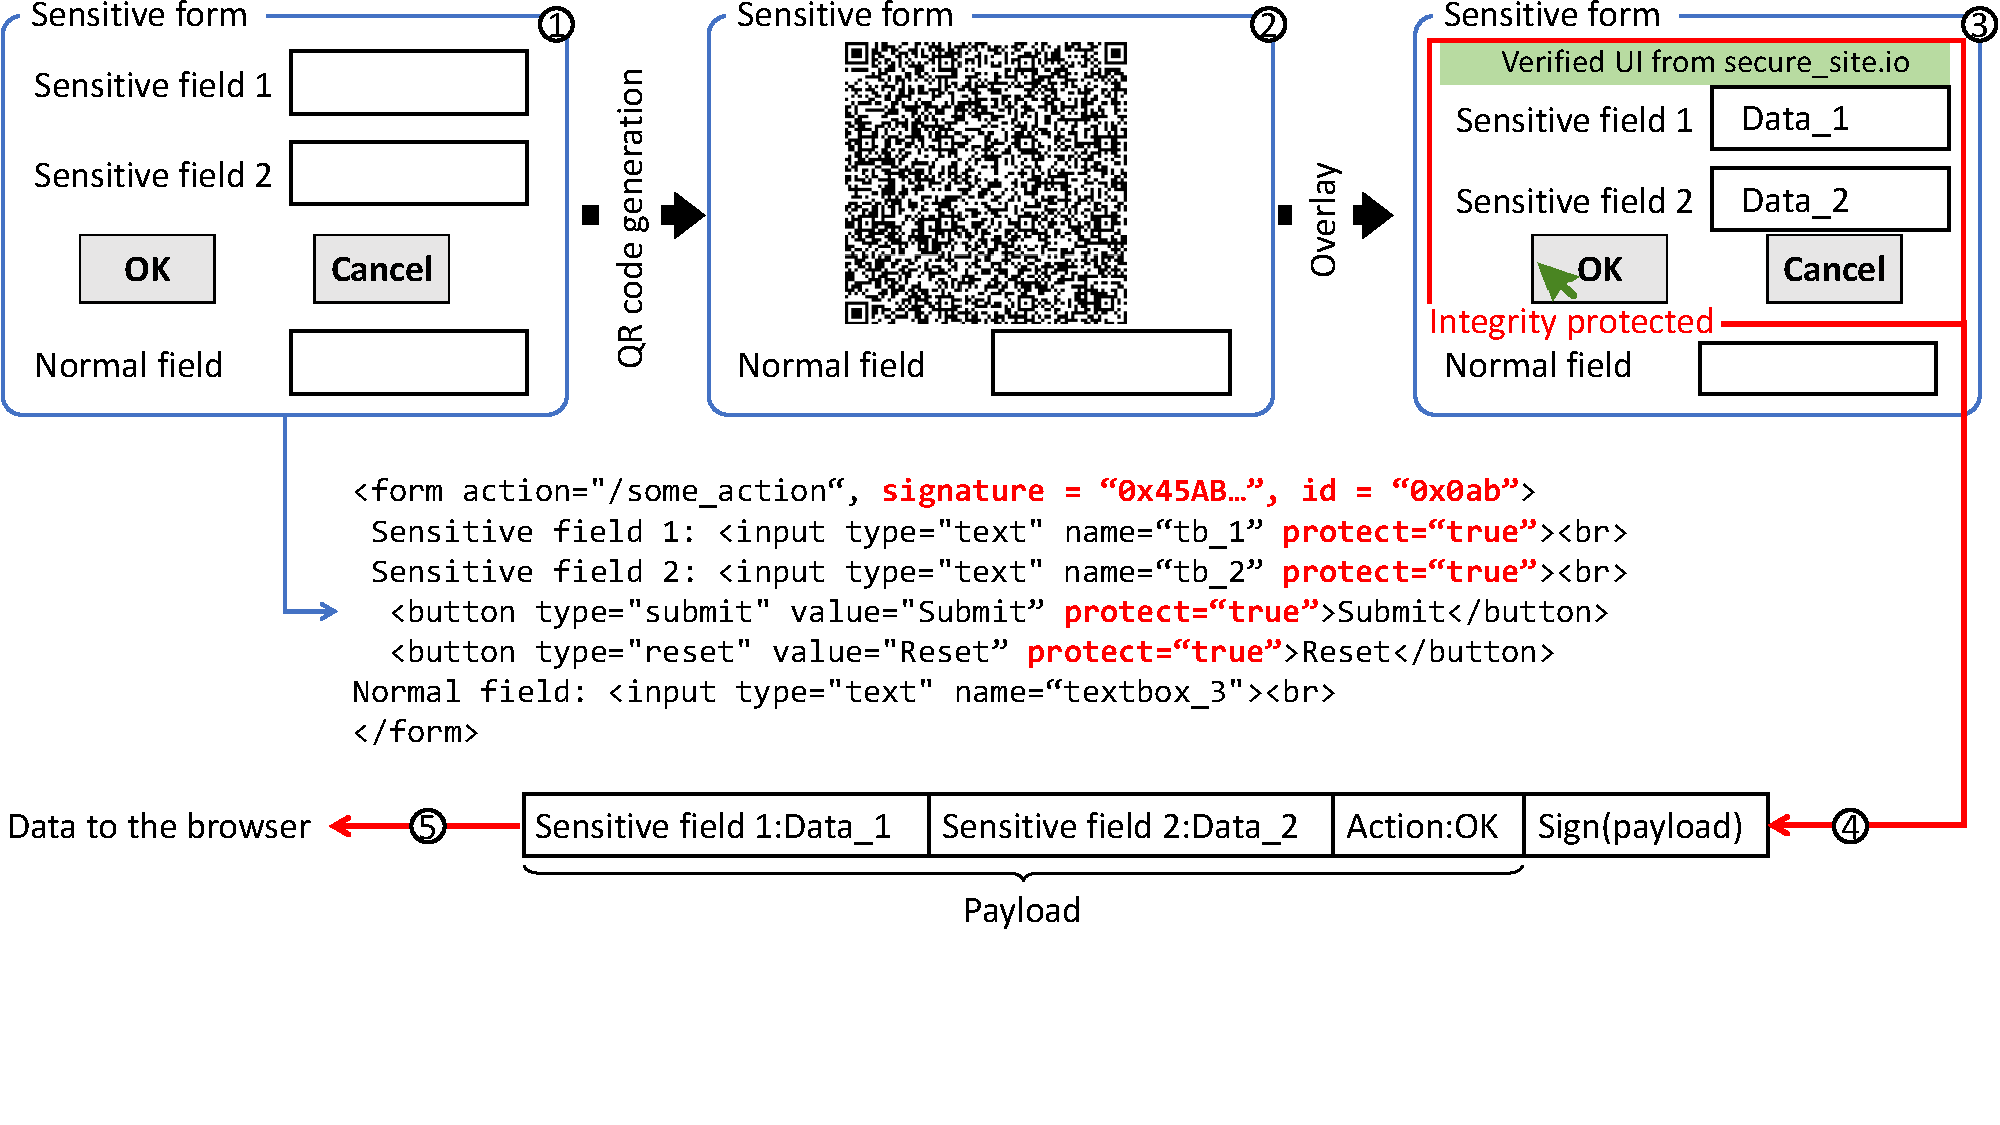
\includegraphics[trim={0 4cm 0 0}, clip, width=\linewidth]{chapters/ProtectIOn/images/formTransform.pdf}
\caption[Transformation of UI elements: HTML $\rightarrow$ encoded specification $\rightarrow$ \device generated UI overlay]{\textbf{Transformation of UI elements: HTML $\rightarrow$ encoded specification $\rightarrow$ \device generated UI overlay.} \one The actual webpage and the corresponding \html source shows the UI elements that requires integrity protection. \two These UI elements are transformed into an encoded UI specification (our \name prototype uses QR code that encodes a UI specification, e.g., Specification~\ref{snippet:UISpecification}) by the \name JS. The QR code. \three AThe QR code decoded and overlaid on the HDMI stream by the \device. \four Upon the user's action on the overlaid UI elements, the device signs all the input data. \five The \device sends these signed input data them to the remote server. Note that the intermediate QR code transformation (\two) is not visible by the user.}
\spacesave
\label{fig:transformation}
\end{figure*}

\section{\name for IO Integrity}
\label{sec:protection}



\lstset{language=JSON, frame=tb, caption=\textbf{Protected UI specification language.} The UI specification shows the JSON formatted UI specification that is generated from the \html source provided in the UI illustrated in Figure~\ref{fig:transformation}., label=snippet:UISpecification, firstnumber =1}

\begin{figure}[t]
\scriptsize
\begin{lstlisting}[mathescape=true]
{ "formId": "form1", "formName": "form1",
  "domain": "secure_site.io",
  "size": "400*400", "SAS": "5:LB",
  "ui": [{"id":"textbox_1", "type":"textbox", 
      "label":"Sensitive field 1",
    "text":"secret data 1",
    "RE":(A-Z)*.(A-Z)*},
    {"id":"textbox_2", "type":"textbox",
    "label":"Sensitive field2 ",
    "text":"secret data 2"},
    {"id":"b1", "type":"button",
    "label":"OK", "trigger":"true"},    
    {"id":"b2", "type":"button",
    "label":"Cancel", "trigger":"false"}],
  "signature": "0x45AB...", "id": "0x0ab.."}
\end{lstlisting}

\end{figure}

%In this section, we provide the technical details of \name for the integrity protection of IO devices. 
In this section, we provide the technical details of \name that guarantees the integrity of IO operations.


\subsection{\device Overlay of UI Elements}
\label{sec:systemDesign:transformation}

As we explained in the previous sections, both output and input integrity are necessary to be protected to achieve any of them. \name ensures output integrity by isolating a part of the display that cannot be observed or modified by the untrusted host. \device intercepts the HDMI frame from the host and injects a render of the sensitive UI on the screen. The overlay provides output integrity because it restrains the attacker from drawing on top of it to trick the user into providing incorrect inputs. 

Our goal is to minimize the TCB, and thus the \device does not run a browser, i.e., it cannot interpret or render HTML, \js, etc. Given this constraint, one strawman solution could be sending UI bitmaps from the server to the \device, and the \device could send back the mouse click and the corresponding location. \device could download these pre-generated form bitmaps from the server, and such a solution would handle static forms, but not for dynamic forms. Downloading all possible form bitmaps would be prohibitively expensive.

To achieve a more generic and efficient solution, we follow a different approach. The \device comes with a small interpreter routine that is similar to render engines of browsers in functionality, but drastically smaller in size because it only renders a limited number of HTML5 UI elements according to their position, dimension, and label. The interpreter routine reads a given specification and renders the respective UI. The specification is a simple \emph{JSON} file that defines how the content of the overlay should be rendered, e.g., number of elements, order, types, and labels.  

The process of rendering the overlay on the screen has two phases: (i) convert the existing sensitive form to specification, and (ii) specification to overlay.

\myparagraph{(i) Secure form $\rightarrow$ Specification} The W3C UI security policy~\cite{w3c_spec} recommends developers to annotate the security-critical UI elements of a page to protect them against malicious JS running on the browser. We use a similar technique by asking developers to manually annotate the sensitive elements in the HTML code (as \emph{protect=``true''} attribute). Then For every request, the \name server-side component parses the HTML source, adds a random identifier (\texttt{id}) to the \texttt{form} element, signs it, add the \texttt{signature} to the \texttt{form} and then delivers it to the user's browser. The \texttt{id} serves as session identification to prevent the attacker from re-submitting an old input data from the user. On the host-side, \name JS parses the tagged HTML source and produces a specification that can be interpreted by the \device.  An example of a specification is presented in~Specification~\ref{snippet:UISpecification}. In our implementation, the \name JS encodes the specification in a QR code. \red{(\#5)We choose QR codes to encode UIs as it is one of many robust ways to encode data on a visual channel such as HDMI stream.} Figure~\ref{fig:transformation} shows the transformation between the step \one and \two. The step \two is processed by \device in the next phase and is not visible to the user.


%We further optimize this process that does not require to add the UI specifications into the HTML sources. The developers include small JavaScript code: \name JS to their sources. \name JS has the same functionally as the server-side code that parses the HTML code and outputs the specification. Note the specification generation process is deterministic, hence, given identical HTML sources, both server and the \name \js generate identical UI specifications. Note that \name JS runs on the browser and is not trusted in our system model. We illustrate the method of UI transformation in Figure~\ref{fig:transformation}. 


\myparagraph{(ii) Specification $\rightarrow$ Overlay} \device performs the next phase, which starts with the detection of the encoded specification (QR-code) in the HDMI frames. Then the \device validates the signature, renders the overlay according to the specifications, and presents it to the user.  The \device overlay is depicted in \three in Figure~\ref{fig:transformation}, which is the final UI shown to the user. Note that the user does not see the QR code as it gets decoded and overlaid by the \device on the fly.

\device uses the specification to determine the particular UI element that the user interacts with. When the user clicks on a text field, \device allows the user to type input to it. UI elements in the overlay take inputs only from input devices (mouse and keyboard). Therefore a malicious host cannot inject or modify any input of the user.

\subsection{Focusing User Attention}
\label{sec:systemDesign:userAttention}

In the previous section, we explain how \name provides output integrity for the overlay generated by the \device. However, the attacker can show fake information to the user on the untrusted part of the display space that may potentially influence her inputs. An advanced adversary could craft malicious directions and present to the user as part of the overlay.

To mitigate these attacks, we employ techniques that are proposed against similar threats in the context of browser-based security. The goal of these techniques is to focus user attention on the sensitive UI elements she is interacting with. Huang et al.~\cite{huang2012clickjacking} proposes two main techniques that are shown to be effective and can easily be adopted by the \device.  The first technique is called Lightbox, and it dims out the non-overlaid part of the screen, which is generated by the untrusted host. The second technique consists of freezing display frames from the host when the user enters into the overlaid UI. This way, a malicious host cannot grab the user's attention by showing an animation or exploiting other tricks.
Lightbox offers more security guarantees because it blocks the untrusted screen completely, but is more intrusive to the user. While freezing is less intrusive but does not remove potential malicious information from the screen.

Lightbox mitigates the attacks presented above. The paper shows that the Lightbox and freezing are effective in $98\%$ and $97\%$ of the time (baseline: $69\%$ effectiveness when no protection is provided), respectively, making them suitable candidates for \name. For more details of the user study, refer to Table 2 in~\cite{huang2012clickjacking}. We assume that a similar result should be expected in \name due to the similarity of the application space (web applications). \device uses Lightbox as the default technique, but depending on the specific form, the developers can select the appropriate technique.

When the focusing mechanism (e.g., LightBox) is active, the user can still interact with the UI elements and browser button outside the secure UI elements as the \device does not control those. Browser back button does not influence the state of the overlaid UI as long as it does not remove/change the QR code on the web page.


\myparagraph{\bfseries Automated activation} The technique to focus user attention (dimming out or freezing the non-overlaid part of the screen) is triggered automatically in specific situations: The user moves the mouse pointer over the overlaid UI, or the user starts typing into a sensitive UI element. 
%e.g., when the user moves her mouse pointer over the overlaid UI, or start moving the mouse after a brief pause (like 5 seconds). 
The advantage of the automated trigger is that the user does not need to remember to activate the mechanism. Hence the system is resilient from user habituation and does not require the user to monitor security indicators actively or perform specific actions. Note that the automated activation provides security to user IO data \emph{only} when the integrity of the data is considered.

\subsection{Continuous Tracking of Mouse Pointer in the HDMI Frame}
\label{sec:systemDesign:analysis}


\begin{figure}[t]
\centering
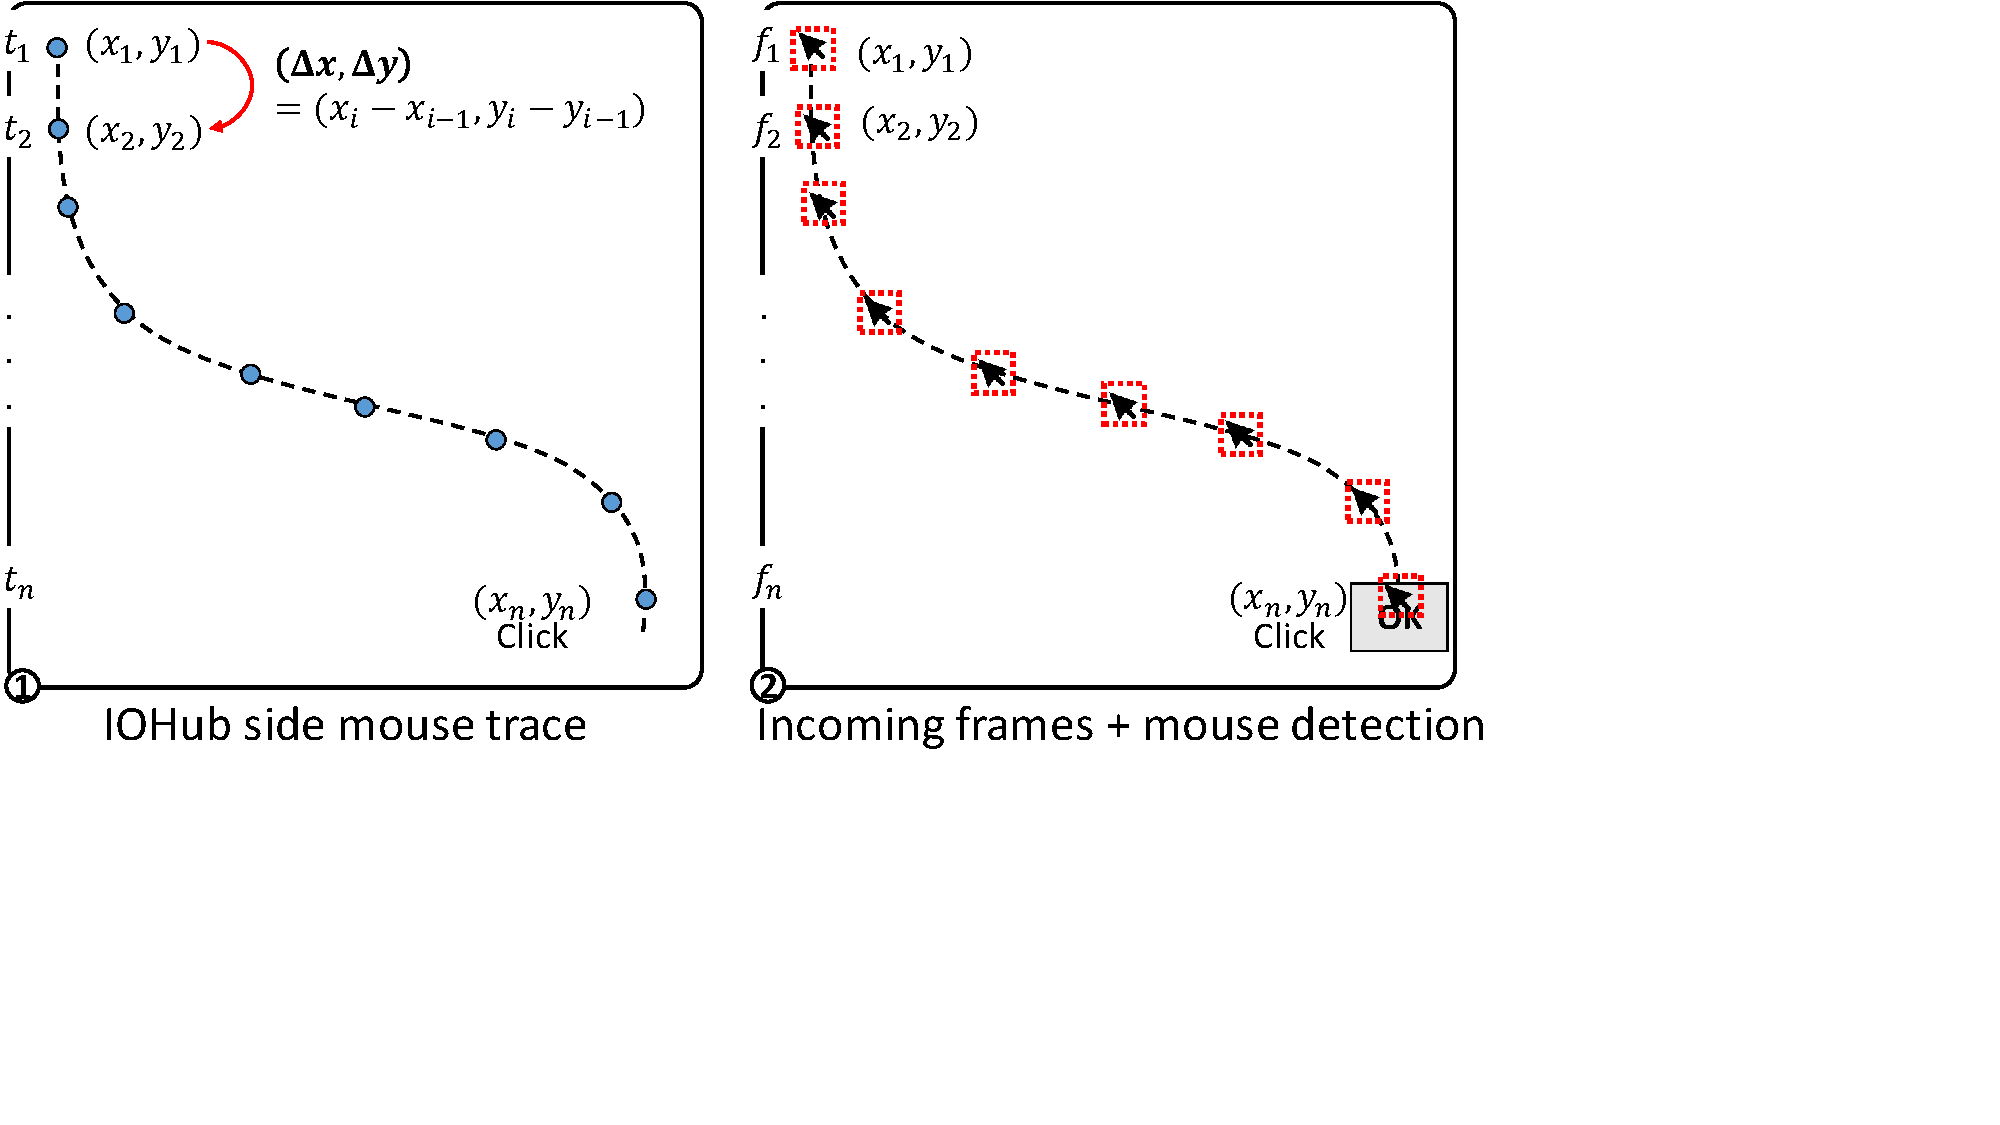
\includegraphics[trim={0 5.2cm 8cm 0}, clip, width=0.9\linewidth]{chapters/ProtectIOn/images/mouseAnalysis.pdf}
\caption[\name Pointer tracking]{\textbf{Pointer tracking.} \one The \device captures the raw mouse events ($\Delta x, \Delta y$) from the mouse that is attached to the \device. \two The \device captures the frames from the HDMI channel and checks into the designated pixel position $(x_i + \Delta x, y_i + \Delta y)$ if there exists a pointer. $t_1, t_2,\ldots t_n$ are the time instances when the \device receives the mouse data. $f_1, f_2,\ldots f_n$ are the corresponding HDMI frames that the \device intercepts.}
\spacesave
\label{fig:mouseAnalysis}
\centering
\end{figure}


The triggering of the focusing mechanism poses a challenging task to \name because the \device does not know the exact position of the mouse pointer. We cannot rely on the compromised host to communicate the pointer position reliably to \device. Furthermore, the host's pointer is not visible when the user interacts with the overlay rendered by the \device as the \device always draws on top of the HDMI frames of the host. 
%To address this issue, \name continuously tracks the host's mouse pointer from the HDMI frame (using shape detection) as it has access to both the HDMI channel and the raw mouse data.

\device could employ image analysis over the frame received from the host to learn the pointer position. However, we avoid this method because image analysis is time-consuming and vulnerable to adversarial images. In our approach, the \device intercepts mouse events and HDMI frames, so it can track the pointer based on mouse data and correlate it with the actual position in the HDMI frame (using shape detection in a small area). Then, the \device overlays a mouse pointer that is prominent and easy to follow by the user. 

A malicious host can still show a fake pointer to trick the user into following it, but when the focusing mechanism is active (the user interacting with sensitive elements), only the pointer overlaid by \device is visible. This way, the pointer tracking and the pointer overlay address three major challenges: i) both the \device and the user have the same sense of the pointer position, ii) \device precisely knows when to trigger the focusing mechanism, and iii) the user can interact with the overlaid UI seamlessly. 


\subsubsection{\bfseries Calibration}\label{sec:systemDesign:analysis:calibration} When the user connects the \device for the first time after booting up, the \device performs an automated calibration to find the pointer. The \device simulates the mouse and pushes the pointer to the top-right corner of the screen. Then the \device searches the pointer at this position in the HDMI frames
%If the \device is successful in finding the mouse pointer, 
and starts tracking the pointer afterward. Note, that at any point, if the \device loses track of the mouse pointer, the \emph{calibration} process is repeated the first moment the user visits a website that employs \name.
%user can recalibrate it by reinitializing the \device.

\subsubsection{\bfseries Pointer detection} The \device ensures pointer integrity by tracking the mouse movements using the raw data from the mouse and the HDMI frame.  Figure~\ref{fig:mouseAnalysis} illustrates the main idea: 

\begin{enumerate}
\item[]\one Shows raw mouse data that notify the displacement events $(\Delta x, \Delta y)$ over $x$ and $y$ axis which are fired over time series $t_1,\ldots, t_n$. Note that the initial pointer position is known to the \device from calibration phase where $(x_0, y_0) = (0, 0)$.  
\item[]\two Shows the HDMI frames $f_1,\ldots f_n$ where the \device expects the mouse pointer to be found. For efficiency, the \device only scans a small portion of the HDMI frames ($200 \times 200$ square pixels) that is enough to cover a mouse pointer. Since the operating system can treat mouse movements slightly different according to their algorithm, this step serves to adjust the position difference.
%\device checks if there exists a mouse inside this square or not. \red{In case there exists a mouse cursor, the \device allows further user interactions; otherwise, it stops all the communications and shows an error on display.}
\end{enumerate}


\subsubsection{\bfseries Overlay of the mouse pointer} The \device draws a mouse pointer overlay on top of the actual mouse pointer. The host mouse pointer is neither visible on top of the overlay nor it can interact with the \device's overlay. The overlaid mouse pointer is visible on top of the overlay, and it offers the same user experience as the host-rendered mouse pointer.


\subsubsection{\bfseries Coping with the disappearing pointer} Many OS offer a feature where the mouse pointer disappears from the screen when the user types in a text editor/browser. When the user moves her mouse, the cursor appears again in the same position where it disappeared in the first place. From the \device's perspective, it is hard to distinguish between this case and the attacker deliberately removing the mouse pointer from the screen. To handle this case, the \device listens to all the keyboard inputs -- the keyboard is also connected to the \device. Therefore, when the \device gets a keystroke event, it expects the cursor to disappear from the screen. Then, \device continues tracking the pointer from the moment that the mouse sends events  - this way, the \device ensures the consistency of the pointer position.  


\subsubsection{\bfseries Handling different mouse cursors} The \device is preloaded with template images of the mouse pointer for detection. For our \name prototype implementation, we use the default cursors provided by the Ubuntu OS. This allows the \device to identify the cursor when it changes on the screen, e.g., from pointer to a hand when the user hovers the pointer over a link on the browser. 

 
\subsubsection{\bfseries Handling mouse acceleration} The \device uses the default mouse acceleration parameters of \emph{libinput} to cope with the pointer acceleration. As the \device emulates itself as a keyboard, at the time of initialization, the \device sends a command to the host to set the default acceleration. In case the host changes the mouse acceleration, the \device will fail to detect the mouse in the HDMI stream. We consider this case as a denial of service.

\subsubsection{\bfseries Entering/exiting secure mode with keyboard} In our implementation of \name, entering and exiting the secure mode is performed by moving the mouse pointer into or out of the protected UI area (sensitive web form). 
%But similar could be done with the keyboard also.
This could similarly be done with the keyboard.
The user could use the \emph{TAB} button that selects the QR code (that is an image on the webpage) on the browser. When the QR code is selected, \name JavaScript triggers a change in the JSON specification that is encoded in the QR code. E.g., the specification contains a parameter named \emph{selected} that defines if the user is inside the secure mode or not. By changing this parameter, the \name JavaScript signals the \device that the user is currently in the secure mode. While inside the secure mode, the \device handles the \emph{TAB} signal from the keyboard, allowing the user to switch UI elements within the secure UI. When the user reaches at the end of the secure UI, the device returns control back to the \name JavaScript when the user presses \emph{TAB}.


\begin{figure}[t]
\centering
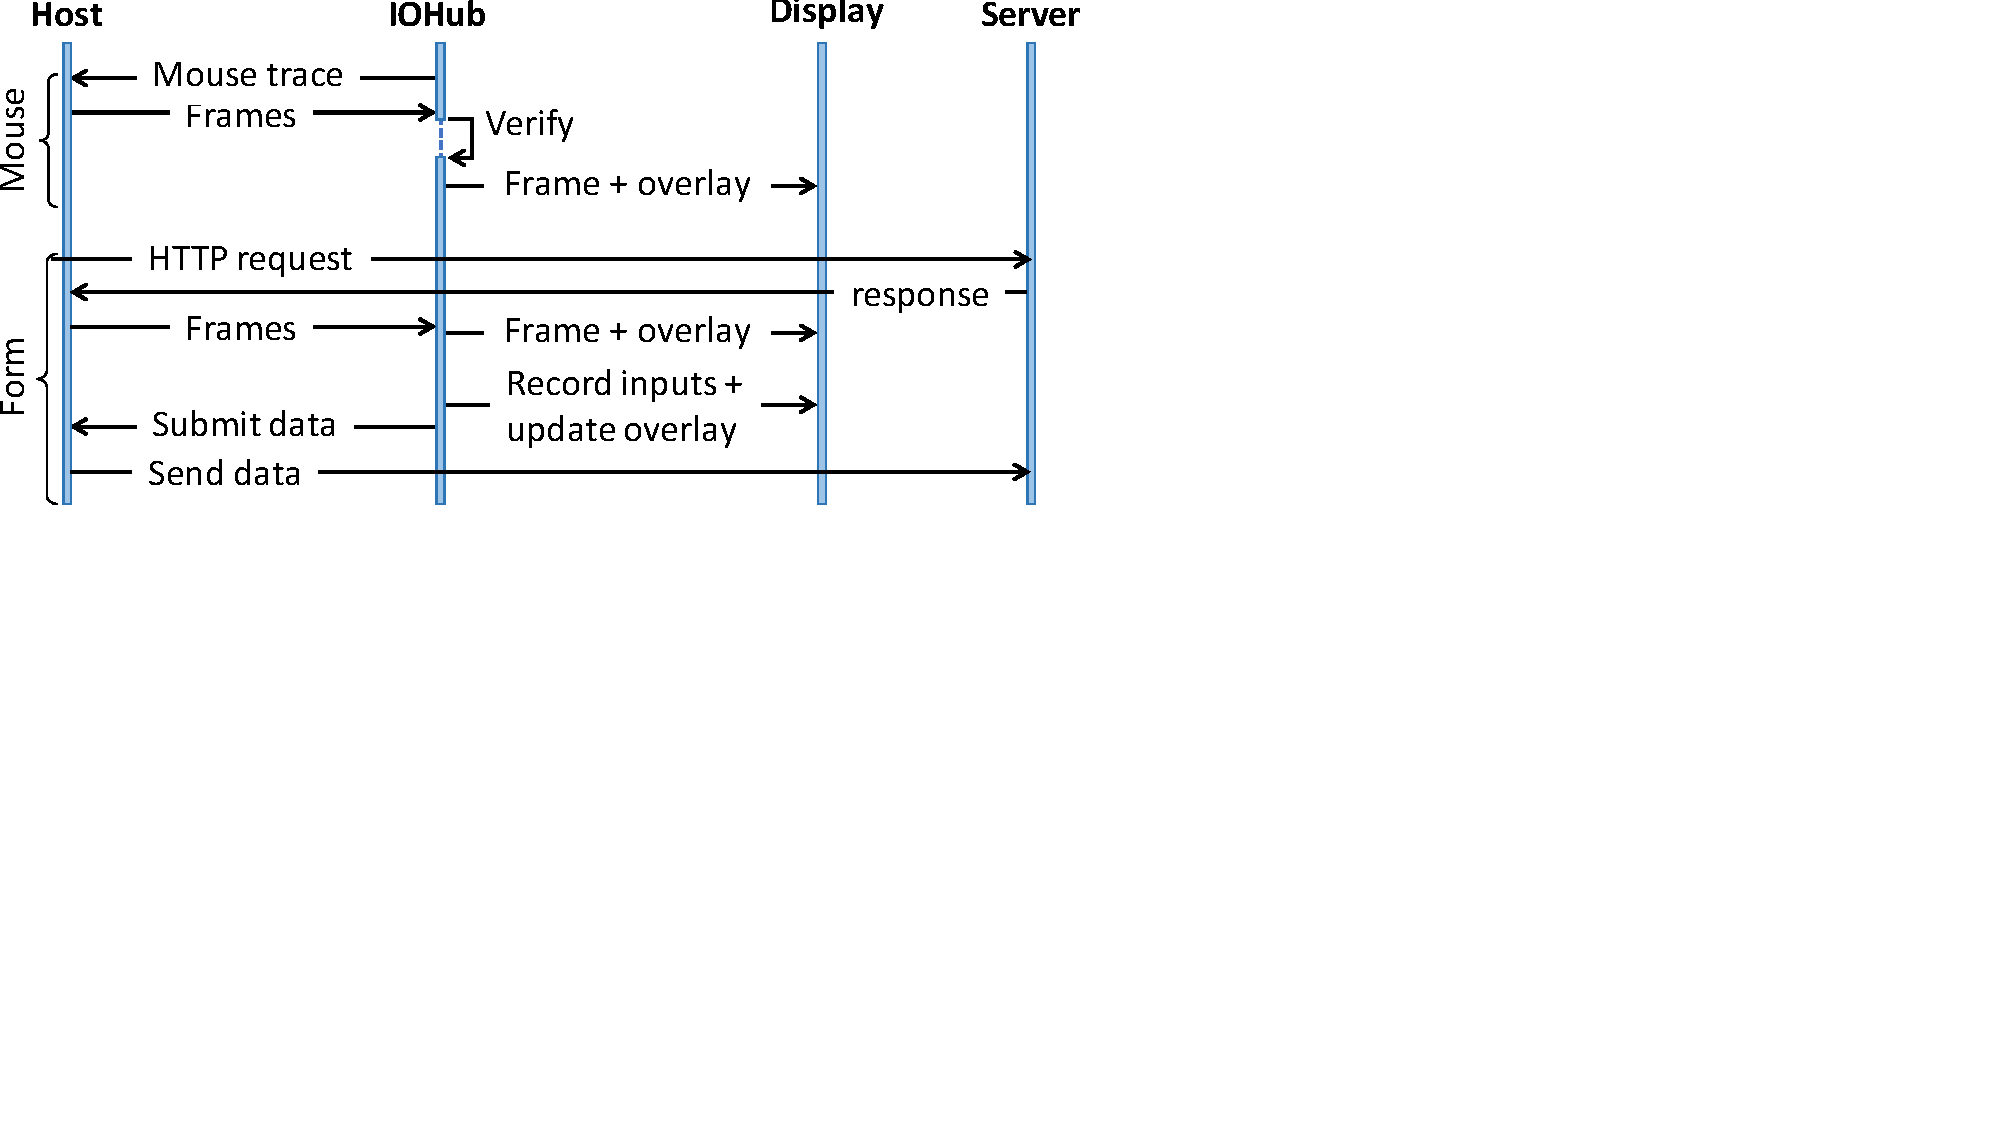
\includegraphics[trim={0 9.5cm 15cm 0}, clip, width=0.85\linewidth]{chapters/ProtectIOn/images/SequencDiagram.pdf}
\caption[Flow of the \name main protocol]{\textbf{Flow of the \name main protocol.} The figure shows the sequence of events for two example scenarios: mouse movement and filling up a web-form.}
\spacesave
\label{fig:sequence}
\centering
\end{figure}


\subsection{Protected User Interaction}
\label{sec:systemDesign:commit}

When the user finishes providing her input via input devices (mouse and keyboard), the \device sends these values (with signature to ensure integrity) to the remote server. Sending these signed input values to the server requires an upstream channel from the \device to the server. 


\subsubsection{Upstream channel}\label{sec:systemDesign:commit:upload} 
The data from the \device to the remote server is transmitted using the \name JavaScript snippet as a helper. 
%The \name JavaScript snippet uses a hidden text field to accept data coming from the \device. 
The \device emulates itself as a composite human interface device (HID) when it is connected to the host. The \device emulates keystrokes that transmit encoded data to the \name JavaScript snippet, which then forwards them to the remote server.


\subsubsection{Sending input data} Figure~\ref{fig:sequence} depicts the user interactions in a sequence diagram. The user input transmission procedure is illustrated in Figure~\ref{fig:transformation}. This has two phases: \emph{record} and \emph{transmit} as described in the following:

\begin{enumerate}
\item \textbf{Record.} After the UI elements are correctly overlaid on the screen, the users can interact with these UI elements. The user interaction with the overlaid UI element is no different than a standard UI. The UI specification encodes the behavior of all generated UI elements, making the \device aware of the semantics of the UI objects. E.g., when a user selects a text box and types on with her keyboard, the \device intercepts all keystrokes and renders the characters on the overlay.
When user enters input data in the rendered overlay UI elements (such as textbox, button, slider, radio button, etc.), the \device records that in a (key, value) pair where the key is the identifier of the UI element (\emph{id} in Specification~\ref{snippet:UISpecification}) and the value is the user provided value. The \emph{type} of the UI elements determines what information to record. For example, the \device records all keystrokes when a textbox is selected, the value corresponding to the position of the slider is recorded when the user interacts with a slider, etc. One example of the recording of the input data corresponding to the UI illustrated in Figure~\ref{fig:transformation} and Specification~\ref{snippet:UISpecification} is: 
\begin{align*}
Record = & (tb\_1, Data\_1);(tb\_2,Data\_2)
\end{align*}

\item \textbf{Transmit.} In the transmit phase, the \device waits for the user to select a UI element that has a \emph{trigger} capability, e.g., a submit button on a web-form. A trigger element can change the state of the overlaid form, e.g., submit the data of the form to the remote server or reset it. More details are provided in the implementation of \name in Section~\ref{sec:prototype:impl:qr}. When the user clicks the \emph{OK} button, the device signs $Record$ with its embedded private key. One such signed packet is also illustrated in Figure~\ref{fig:transformation}. The \device sends the signed packet to the remote server using the upstream channel.
\end{enumerate} 

%\subsubsection{\bfseries Server-side verification} \label{sec:systemDesign:commit:verification}
Upon receiving the signed input data from the \device, the remote accepts the input if the signature verification is successful. Note, if an input field is annotated as \texttt{protect=``true''}, the server does not accept any input without the \device signature. This prevents the attacker-controlled host to submit data. 


\subsubsection{Changing browser tabs or browsers}
The \device supports multiple browsing tabs across multiple browsers. The UI specification contains \emph{formId} and \emph{domain} that works as the unique identifier for a specific form served from a specific web server. The \device can maintain multiple parallel TLS connection to web servers. Depending on the observed \emph{formId} and \emph{domain} (refer to Specification~\ref{snippet:UISpecification}), the device retrieves the data that is entered by the user. This way even if the user switches tabs, the \device can still allow editing the forms across tabs.


\subsubsection{Input validation} Input validation, i.e., checking the input against a recommended input policy (e.g., regular expression) is one of the most widely used JavaScript functionalities, and it is a critical part of input integrity. The remote server sends the regular expression in the UI specification (\emph{RE} in Specification~\ref{snippet:UISpecification}) that the \device uses to validate the user input.

%\myparagraph{Sequence of Events} In the previous sections, we explain the basic components of \name. Here we summarize the overall flow of the system. The sequence diagram of \name is illustrated in Figure~\ref{fig:sequence} that shows snapshots of two example sequences: mouse movement and filling up a web-form.


\subsubsection{Fallback for legacy clients} \name is backward-compatible with the clients who do not use the \device. This is achieved by the remote server by showing a QR code briefly on the screen when the user visits the \name-enabled webpage. The \device intercepts the QR code and sends a signal to the server about its presence. In the absence of the \device, the remote server does not send the \name JS to the host that acts as a communication channel between the \device and the remote server. Note that the fallback mechanism is application-specific, and the service provider could decide if the fallback is detrimental to security.


\section{\name Software design}
\label{sec:programmingModel}

% \ad{Attestation and platform awareness part is revised. Continue with the motivation}

In this section, we introduce \name{}'s software design which is one possible way for the application, driver, and firmware developers to adapt their software to be compatible with \name without making a significant changes.  

% \begin{figure}[t]
% \centering
% 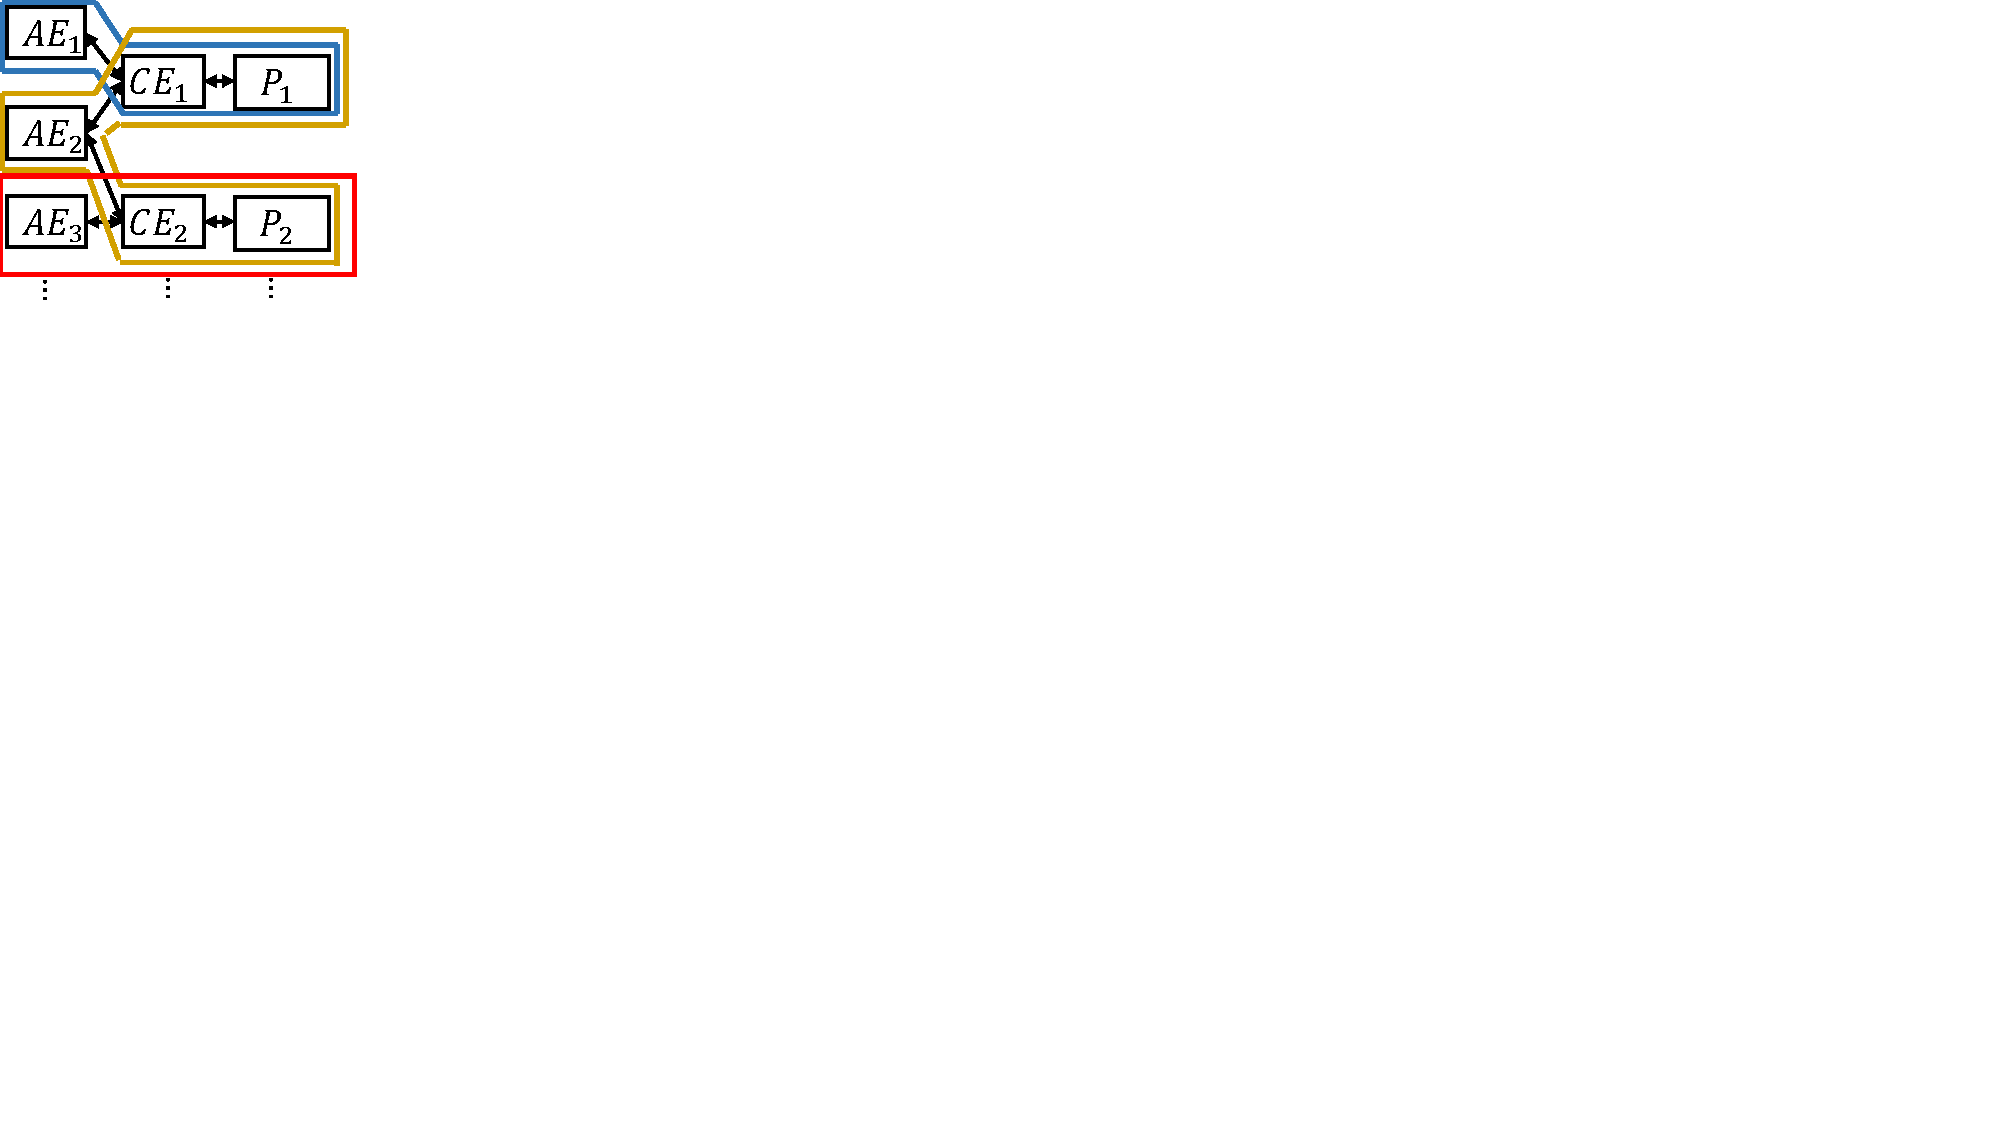
\includegraphics[trim={0 14cm 27cm 0}, clip, width=0.5\linewidth]{programmingModelComponents.pdf}
% %\caption{\textbf{\Nameenclave{}s in the \name{}'s software design.} The application enclaves (AE) contain the application logic and communicate with \sphw through a controller enclave (CE) that contain the driver logic for the specific \sphw. In our software design, we assume that there is only one \ce per \sphw. Multiple \app can connect to one \ce{}, and one \app can connect to multiple \ce. Three separate \nameenclave{}s are indicates by the blue, yellow and red outlines.}
% \vspace{-1em}
% \caption{Three example \nameenclave{}s in \name{}'s software design with \app{}s (AE), \ce{}s (CE), and \sphw{} devices (P). Note that the yellow \nameenclave{} is spanning two external devices. It is the responsibility of the \ce{}s to isolate the data from the different \app{}s.}
% \label{fig:programmingModelComponents}
% \end{figure}

\subsection{Software components}
\label{sec:programmingModel:systemComponents}

\name's software design consists of three entities: \app{}s, \ce{}s, and \sphw firmware as shown in Figure~\ref{fig:sharedMemory}. \app{}s and \ce{}s are processor-local enclaves. \sphw are the components that are connected to the platform over buses. Contrary to a monolithic design where the application and driver is in one big enclave, our modular approach aims to provide high flexibility and increase code reuse.


\myparagraph{Application enclaves} \App{}s are similar to the traditional enclaves in Intel SGX or Keystone. In such TEEs, the enclaves cannot access \sphw without using the OS as a mediator, as the OS handles all drivers. In \name, \app{}s also cannot communicate with a \sphw directly. The \app{}s use shared memory to communicate with a \ce that is a \sphw-specific enclave containing the driver logic. The rationale of separating the driver from the application logic is two-fold, i) to avoid requiring the developers to ship driver code with their application, and ii) one \ce per \sphw allows multiple \app{}s to communicate with that specific \sphw in parallel. %Note the processor may employ memory encryption to encrypt all shared memory regions to protect against a local physical attacker. However, the developer could also add an additional encryption layer on top in order to make the data accessible only between the application enclave and the \sphw (where the \ce works as the untrusted transport layer between the \app and the \sphw). 


\myparagraph{Controller enclave} The \ce contains the driver that facilitate communication with a \sphw. Note that \app{}s, standard non-enclave applications, and the OS cannot access the \sphw directly. The only way to communicate with a \sphw is through a device-specific \ce. Such a design choice isolates the \sphw drivers: one compromised driver does not affect other \sphw. The \ce maintains an isolated communication channel over shared memory (e.g., in RISC-V, the PMP entry corresponding to a shared memory ensures that only participating enclaves have access to that shared memory) to \app{}s and the \sphw. To simplify the configuration, we assume that only one active \ce per \sphw exists at a time. However, any \ce can be replaced at the user's request. %Note that \ce is the only way to access a specific peripheral. All the other non-enclave applications running on the OS need to connect the \ce (in contrast to the standard OS device driver) to access a peripheral.  

\myparagraph{Isolation of multi-\app session}\label{sec:programmingModel:systemComponents:multiApp} In \name, multiple \app{}s could connect to a single \ce to have simultaneous access to a \sphw. In such a scenario, the \ce keeps separate states corresponding to each of the \app{}s. Note that this is primarily a functional and then a security requirement as operations in one \app could affect the state of computation of another \app in case there is no isolation. For some \sphw, the \ce may need to reset the state of the \sphw when it switches to a session with a different \app (temporal separation). However, for \sphw such as GPU that support multiple isolated workloads in parallel, the state does not have to be reset.


\subsection{Platform-wide attestation in the software design}

The platform-wide attestation enables a remote verifier to verify the state of the all \nameenclave components. The attestation proceeds as the following:


\myparagraph{Remote attestation of the \app} This is the first step of the  platform-wide attestation to ensure that the platform is running the intended version of the \app. The \app attestation report includes the list of identifiers of the \ce{}s that have shared memory channels with that \app.
    
\myparagraph{Remote attestation of the connected \ce{}s} The user then executes a series of individual remote attestation for the \ce{}s. The \ce{}s send the attestation report of themselves along with the certificate that is received from the connected \sphw. These reports are signed by the same platform key as of the \app attestation report. This proves that the \app and the connected \ce{}s are running on the same physical platform. Additionally, the \ce also states that the initiating \app has a shared memory channel with it.

 For each remote verifier, the TCB is constrained to only the specific \nameenclave that she is verifying. Hence a remote verifier does not need to trust any \app, \ce or peripheral that she is not using/attesting

%===========================================================================================================
% \paragraph{Remote attestation of the \app} The platform-wide attestation process starts with the verifier who wants to attest the deployed \app. The purpose of the remote attestation of the \app is to ensure that the platform is running the intended version of the \app. The \app attestation report includes the list of identifiers of the \ce{}s that have shared memory channels with that \app. This report is signed by the platform's private key. 

% \paragraph{Remote attestation of the connected \ce{}s} As mentioned above, the user receives a list of identifiers of \ce{}s that have shared memory channel with the \app. The user then executes a series of individual remote attestation for the \ce{}s. The \ce{}s send the attestation report of themselves along with the certificate that is received from the connected peripherals. These reports are signed by the same platform key as of the \app attestation report. This proves that the \app and the connected \ce{}s are running on the same physical platform. Additionally, the \ce also states that the initiating \app has a shared memory channel with it. At the end of this process, the verifier who initiated the remote attestation of the \app receives the signed attestation report of the said \app, all the \ce{}s that are connected with the \app and all the peripherals that are governed by the \ce{}s.

% \paragraph{Local attestation between \ce and peripheral} The local attestation process between a peripheral and a \ce takes place when a new peripheral is attached to the platform. This step is independent of the above mentioned two steps that only starts when the verifier wants to attest a specific \app. When a new peripheral is attached to the platform, \ce gets the list of attached peripherals from the SM (through the device tree). The peripherals come with a certificate that states the firmware version certified by the manufacturer along with the signing key from the manufacturer. The \ce issues a random challenge to the peripheral. It verifies if the peripheral actually owns the private key corresponding to the certificate. The peripheral signs the challenge and sends it back to the \ce for verification.
% After the local attestation between the \ce and the peripheral, the \ce knows that is it connected with a legitimate peripheral with a certified firmware.



% \paragraph{Peripherals} 
% \label{sec:programmingModel:systemComponents:peripheral}

% We consider on-chip peripherals as well as external peripherals that are attached to the platform. However, we require them to store some key material from the manufacturer securely for attestation. Similar to \app{}s, peripherals also share memory regions with the \ce that is used as a communication channel. The firmware that runs on peripherals is also part of the platform-wide enclaves. For simple peripherals such as IO devices (keyboard, mouse, etc.), GPS, and temperature sensors, the modification in the firmware is minimal. Essentially, this only includes adding a certificate from the manufacturer that proves that the peripheral is running the correct version of the firmware. %However, for complex peripherals such as GPUs, the developers may require to change the firmware as the GPU needs to isolate the data from multiple \app{}s that execute operations on the GPU simultaneously.



% \subsection{Platform-wide Attestation}
% \label{sec:programmingModel:attestation}

% In Section~\ref{sec:approach:attestation}, we provide the hardware construct for \name{}'s platform-wide attestation. In this section, we describe how it related to the programming model components. The platform-wide attestation that enables a remote verifier to verify the state of the \nameenclave components - \app{}s, \ce{}s, and peripherals. Precisely, the state includes the state of the components of the programming model components and their communication channel (over shared memory in our case). Note that there could be more than one verifier (an example is depicted in Figure~\ref{fig:new_system} with two remote verifiers and two \nameenclave{}s) corresponding to several \nameenclave{}s on the same platform. For each remote verifier, the TCB is constrained to only the specific \nameenclave that she is verifying. Hence a remote verifier does not need to trust any \app, \ce or peripheral that she is not using/attesting. Note that platform-wide attestation is built on top of the attestation scheme of the underlying TEE, e.g., the attestation in RISC-V Keystone or Intel SGX. %Enabling  platform-wide attestation requires some modifications of the existing remote attestation procedure of traditional TEEs. 




\section{Security Analysis}
\label{sec:securityAnalysis}

In this section, we will informally analyze the security of \name. We divide the security analysis into two parts based on two security properties: interity and confidentiality.

\subsection{Integrity}
\label{sec:securityAnalysis:integrity}

First we look into the integrity property.

\myparagraph{Modifying IO operations} As only the \device can interact with the overlaid UI, the attacker can not manipulate the IO operations with the overlaid UI. Moreover, the attacker cannot submit arbitrary data to the remote server because the latter accepts only inputs signed by the \device.


\myparagraph{Early form submission} This attack is not possible as the input devices (both mouse and keyboard) are connected to the \device, and only the \device can interact with the overlaid UI. This makes it impossible for the attacker to emulate a click on the overlaid part of the screen.  


\myparagraph{Attack on the mouse pointer tracking and overlay} 
The attacker may try to defeat the \name pointer tracking and overlay mechanism described in Section~\ref{sec:systemDesign:analysis} by introducing a malicious pointer that is visually more appealing to the user. Note that the \device overlaid mouse pointer is prominent and hard to miss. One can visualize it as an arms race between the attacker and the \device to grab the user's attention. We argue that this is a suboptimal strategy for the attacker as both of the pointers will be visible on the screen that causes suspicion to the user. Also, when the real mouse pointer enters the overlaid area, the untrusted part, including the malicious mouse pointer, will be hidden by the focusing mechanism. Hence, we can conclude that executing clickjacking-like attacks is not possible in \name.


\myparagraph{Replay attack} The remote server adds a random identifier (\texttt{id}) in the form specification alongside the signature. With this identifier, the server keeps track of the user input. When the server receives a form submission data, it first checks if the user submitted with the same identifier sent by the server. Otherwise, the server rejects the data. 


\myparagraph{Not rendering QR code} The host may deny sending the QR code over the HDMI channel. We consider this to be a denial of service and does not compromise the integrity of the IO data. 


\myparagraph{Redirection} The attacker could redirect the user to a phishing website that renders visually identical UI to that of the legitimate website. A redirection attack cannot break the integrity of the input because a legitimate remote server always requires the signed input from the user. Without a valid signed specification, the \device never renders an overlay or sign any input. 

\myparagraph{Malicious instruction on the screen} The attacker may put a malicious instruction/label on the untrusted part of the screen to influence user inputs. However, when the user starts interacting with the overlaid UI, the default focusing mechanism (Lightbox) highlights only the secure UI and hides the rest of the screen. 
%The user attention focusing mechanisms enable the user to distinguish the trusted part of the screen from the untrusted part.


\myparagraph{Replication of Lightbox} The attacker can replicate the lightbox on any part of the screen. However, this does not compromise the integrity of the input as the legitimate remote server only accepts signed input from the \device. 


\myparagraph{Multiple HIDs} The attacker can emulate multiple HIDs to avoid the tracking of the mouse pointer. However, this attack is ineffective as the \device only tracks the mouse pointer that is connected to it (over USB interface). 


\myparagraph{BadUSB} BadUSB~\cite{badUSB} is out-of-scope of this paper as in the attacker model (Section~\ref{sec:approach:systemAttackerModel}), we assume that all the IO devices that are connected to the \device are trusted.

\myparagraph{Mouse acceleration/updates} The attacker can change the mouse acceleration or provide erratic mouse updates on the screen. Such manipulations only cause the \device to lose track of the mouse pointer and stop relaying the mouse signal to the host altogether. The \device uses the acceleration parameters from the default \texttt{libUSB} driver to cope with the mouse acceleration. Hence, such manipulation does not affect security.

\myparagraph{Malicious QR codes} The attacker may put fake QR codes on the webpage. Note that the \device verifies the signature from the HTML forms to check the integrity using the pre-configured or white-listed server certificate. This way, the \device does not render any overlays from malicious QR codes.


\subsection{Confidentiality}
\label{sec:securityAnalysis:confidentiality}

\myparagraph{Redirection} The attacker could redirect the user to a phishing website that renders visually identical UI to that of the legitimate website. Redirection compromises the confidentiality of user inputs only when the user does not trigger the SAS mechanism. The \device is only activated when it detects specifications signed from the whitelisted (maintained in the memory) servers.
%Note that the \device contains a whitelist of the remote server addresses and their corresponding certificates. The \device is only activated when it detects specifications signed from the whitelisted servers.
%as the confidentiality of inputs requires the user to manually trigger the SAS to detect any sensitive UI elements that are overlaid by the \device.


\myparagraph{Fake SAS instructions} The attacker may put fake instructions on the screen that attempt to trick the user into typing a false SAS sequence and then revealing her sensitive information to the attacker. This attack is not possible as long as the user follows the instructions it received from the issuer of the \device and only types in secrets after using the correct SAS value (such as \texttt{Ctr+Alt+Del}). Recall from Section~\ref{sec:confidentiality:SAS} that the SAS value is defined by the issuer of the \device and that the SAS keystrokes are always first intercepted by the \device. (The user is expected to trigger the SAS only when there exists a QR code on the screen that is correctly signed by the remote server. In case there is no QR code or a malformed QR code on the screen, the \device warns the user.)


\myparagraph{Side-channel leakages} Even though, the \device ensures that no mouse or keyboard event arrives at the untrusted host when the user executes some operation over the overlaid UI, one can not rule out all side-channel leakages. Depending on the application, the amount of time that the user spends or the entry/exit position of the mouse pointer may reveal some information to the attacker. 
\device could allow the remote server to specify additional policies in the specification to prevent such side-channel attacks, e.g., a minimum amount of time that the device should not forward any event to the host after the user enters the overlay. We leave as future work defining such policies and integrating them on \name.
%However, for fixed-length inputs such as the pin codes or credit card details, do not leak any information about the input.


\myparagraph{Mode Switching} The host could remove the QR code when the user is typing confidential data in the sensitive form. The absence of the QR code makes the \device to assume that the secure session has ended, and the \device forwards the plaintext keystrokes and mouse movement to the host. To prevent the leakage of the input data, the \device continues to overlay and operate on the overlay until the user clicks submit or cancel (or any UI element that has a \texttt{trigger}  capability). This way, the \device locks the UI from the attacker until the user finishes her session.

\subsection{Attacks toward \device} 
\label{sec:securityAnalysis:device}

In \name trust model, we assume that the \device is trusted. However, in the real-world, embedded systems are often vulnerable to attacks as the attacker can use the connection interfaces to reprogram the \device. It is also possible to develop the \device using formally verified languages such as embedded Rust. However, we consider making a security-hardened \device is engineering intensive and out-of-scope of this paper. 


\myparagraph{Downgrade attack} The host can block the initial QR code from the server to the \device. By doing so, the host forces the server to downgrade the security of the webpage, i.e., not serving the \name JS. For integrity, this is not a security threat as the server does not accept any input from the host that is not signed by the \device. Hence, the downgrade attack works as a denial of service, which is out-of-scope of this paper.
%The fallback mechanism, i.e., the case where the user does not have the \device, is outside the scope of this work because it is specific to the policy of service providers. E.g., a bank could issue a new \device for the user, while an online shopping site could allow the user to enroll a new \device or allow access only to nonsensitive functionalities. 


\subsection{Proof for IO Integrity}
\label{sec:securityAnalysis:proof}

In this section, first, we provide a formal proof of the following property: \emph{without protecting both input and output integrity, none of them can be achieved}. 


%\subsection{Interaction Protocol} 
%\label{appendix:security:protocol}

\myparagraph{Interaction protocol}

To simplify the proof, we model the interaction between the user, the host, and the remote server as a finite state automaton (FSA).
The interactions between the server (\server), the user (\user) and host (\host) are depicted in the FSA in Figure~\ref{fig:fsm}.

\begin{figure}[h!]
\begin{center}
\begin{tikzpicture}[shorten >=1pt,node distance=3cm,on grid,auto]
  \tikzstyle{every state}=[fill={rgb:black,1;white,10}]

    \node[state,initial]   (q_1)                    {\user};
    \node[state] (q_2)  [right of=q_1]    			{\host};
    \node[state,accepting]           (q_3)  [right of=q_2]    {\server};

    \path[->]
    (q_2) edge [bend left]  node {$[m']$}    (q_1)
    (q_1) edge [bend left]  node {$(I,[m'])$}    (q_2)
    (q_2) edge [bend left]  node {$(I,[m'])$}    (q_3)
    (q_3) edge [bend left]  node {$m$}    (q_2);
\end{tikzpicture}
\end{center}
\caption[\name protocol FSM]{Finite state machine that depicts the interaction between the user (\user), host (\host) and the server (\server).}
\label{fig:fsm}
\end{figure}


% \begin{figure}[h!]
% \begin{center}
% \begin{tikzpicture}[scale=0.15]
% \tikzstyle{every node}+=[inner sep=0pt]
% \draw [black] (66,-23.1) circle (3);
% \draw (66,-23.1) node {\server};
% \draw [black] (66,-23.1) circle (2.4);
% \draw [black] (45.2,-23.1) circle (3);
% \draw (45.2,-23.1) node {\host};
% \draw [black] (26.9,-23.1) circle (3);
% \draw (26.9,-23.1) node {\user};
% \draw [black] (47.743,-21.516) arc (116.95563:63.04437:17.332);
% \fill [black] (47.74,-21.52) -- (48.68,-21.6) -- (48.23,-20.71);
% \draw (55.6,-19.13) node [above] {$m$};
% \draw [black] (29.352,-21.382) arc (118.8302:61.1698:13.89);
% \fill [black] (29.35,-21.38) -- (30.29,-21.43) -- (29.81,-20.56);
% \draw (36.05,-19.16) node [above] {$[m']$};
% \draw [black] (42.565,-24.526) arc (-66.78269:-113.21731:16.527);
% \fill [black] (42.57,-24.53) -- (41.63,-24.38) -- (42.03,-25.3);
% \draw (36.05,-26.36) node [below] {$(I,[m'])$};
% \draw [black] (63.369,-24.535) arc (-65.91058:-114.08942:19.034);
% \fill [black] (63.37,-24.53) -- (62.43,-24.4) -- (62.84,-25.32);
% \draw (55.6,-26.69) node [below] {$(I,[m'])$};
% \end{tikzpicture}
% \end{center}
% \caption[\name protocol FSM]{Finite state machine that depicts the interaction between the user (\user), host (\host) and the server (\server).}
% \label{fig:fsm}
% \end{figure}

We consider a setting where the user \user interacts with \server over browser through web UI. Hence we assume that all the messages ($m$ or $m'$) exchanged between the user \user, host \host and server \server is HTTP request and response payload. The HTTP response payloads (originating from \server) contains HTML, JavaScript, CSS and other data to construct the webpage at the host's browser. The protocol starts with \user sending an initial request to \server that is delivered through \host. We denote $[m]$ to be the render of $m$ by the \host, i.e, graphical render of the webpage ($m$) on the host's display. In this initial stage consider $[m'] = \phi$. Upon receiving the initial request, the server \server replies with a message $m$ to \host. As \host is malicious, it can transform $m$ to $m'$. Note that this transformation from the message to render to the user's display is a public knowledge and is deterministic. Hence, for a message $m'$, where $m\neq m'$, then given the corresponding renders $[m']$ and $[m]$, \server can determine that $[m]\neq [m']$. We denote the user input to be $I$, which corresponds to a specific $[m]$. 
%Note that the communication channel between \server to \user is neither authenticated, neither confidential. But the communication channel from \user and \server is authenticated. 
In this model, we simplify the user input by assuming that the \user only provides an input $I$ only after observing a message transformation $[m]$. The user provides both her input $I$ and transformation $[m']$ observed by her to \host. The interaction loop between \host and \user can continue until \user finishes her input. After every input \host hands over new message transformation to \user (either result of the input or new message from \server or both). This simulates the changes in the web UI when the user starts interact with it e.g., input feedback. Once the user provides all her inputs, \host send the sequence of pairs $(I, [m'])$ to \server.

To smmarize the interaction protocol above, we define these two mappings as the following:

\begin{align*}
\texttt{Input()}&:[m]\rightarrow I \\
\texttt{Transform()}&:m,I\rightarrow [m'],\ \exists i\in I:i=\phi
\end{align*}
Both of them are \emph{bijective}.

One trace of the protocol transcript mentioned above is depicted in Figure~\ref{fig:protocol}. As described in the FSM (refer to Figure~\ref{fig:fsm}), \server receives a trace of message transformations $([m']_1,[m']_2,\ldots,[m']_n)$ and corresponding inputs ($I_1,I_2,\ldots,I_n$). From these traces \server could determine of all the $[m']_i$ are in proper form by verifying if $[m]_i=[m']_i$.

Given the interaction protocol, we can now formally define the definitions in this chapters such as the input intergity and output intergerity as the following:

\begin{figure}[t]
\begin{center}
\tikzset{
  every picture/.append style={
    transform shape,
    scale=1
  }
 }
\begin{sequencediagram}
\newinst{u}{\user}
\newinst[3]{h}{\host}
\newinst[3]{s}{\server}
\mess{s}{$m$}{h}
\mess{h}{$[m']_1$}{u}
\mess{u}{$I_1,[m']_1$}{h}
%\mess{h}{$[m']_2$}{u}
%\mess{u}{$I_2,[m']_2$}{h}
\mess{h}{...}{u}
\mess{u}{...}{h}
\mess{h}{$[m']_n$}{u}
\mess{u}{$I_n,[m']_n$}{h}
\mess{h}{$I_1,I_2,...,I_n$}{s}
\mess{h}{$[m']_1,[m']_2,...,[m']_n$}{s}
\end{sequencediagram}
\end{center}
\caption[\name protocol transcript]{Protocol transcript between the \server, \user and \host that shows one trace from the FSM depicted in Figure~\ref{fig:fsm}.}
\label{fig:protocol}
\end{figure}


\begin{definition}{\textbf{Input integrity}}
\label{def:inputIntegrity}
Assume that \server handed a message $m$ to \host where the proper message transformation is $[m]$. The host changes the message transformation to $[m']$ where $[m']\neq [m]$. We also define correct \user input to be $I$ when \host sends a correct message transformation $[m]$ to \user. We define input integrity as the property where the \server does not accept input $I'$ where $I'\neq I$from \user if the \host changes the message transformation.
\end{definition}

\begin{definition}{\textbf{Output integrity}}
\label{def:outputIntegrity}
Assume that \server handed a message $m$ to \host where the proper message transformation is $[m]$. Output integrity defines that in all circumstances, \user receives the correct message transformation $[m]$ from \host.
\end{definition}

\myparagraph{Verification process} After receiving all the traces, \server checks $\forall i=1\ldots n$, if $$[m']_i =^? \texttt{Transform}(m_{i-1}, I_{i-1})$$ where $I_0=\phi$.

\begin{lemma}
\label{theorem:th1}
If \user does not send all the transformations till $[m']_i$ corresponding to the input $I_i$, input integrity can not be achieved. 
\end{lemma}

\begin{proof}
If \user does not attach all the transformation till $[m']_i$, i.e., $$[m']_1, [m']_2, \ldots, [m']_{x+1}, [m']_x, [m']_{x-1}, \ldots, [m']_{i-1}, [m']_i$$  corresponding to inputs $I_1, I_2,\ldots, I_{x-1}, I_x, I_{x-1}, \ldots, I_{i-1}, I_i$, then the server can not verify all the transformations corresponding to the input. \host could modify a specific $[m]_x$ to influence \user input. Hence, the following verification will be missing:
$$[m']_x=^?\texttt{Transform}({m'}_{x-1}, I'_{x-1})$$
Where the \host changes message $m$ to $m'$ influence the the user to change her input from $I_{x-1}$ to $I_{x-1}$. Hence input integrity can not be achieved.
\end{proof}

\begin{lemma}
\label{theorem:th2}
If the channel from \user and \server is not authenticated, input integrity is not achievable. But the channel from \server to \user does not require to be secure as long a \user provides the message transformation $[m']_i$ corresponding to every input $I_i$.
\end{lemma}

\begin{proof}
The proof is trivial. If the channel from \user to \server is not authenticated, any input provided by \user can be manipulated by \host without a trace. Hence input integrity is not achievable. As long as \user sends message transformation along with the input, a manipulated message transformation bt \host would be detectable by \server (see Lemma~\ref{theorem:th1}).
\end{proof}

\begin{lemma}
\label{theorem:th3}
Ensuring output integrity also ensures input integrity provided there is an authenticated channel from \user to \server.
\end{lemma}

\begin{proof}
This proof is also trivial. As we describe in the Definition~\ref{def:inputIntegrity} and~\ref{def:outputIntegrity}, if all the message transform from \host $[m']=[m]$, and \host always executes \texttt{Transform()} properly, the input integrity is preserved. As \name ensures output integrity and all the input from the user is signed by the \device, \name preserves input integrity. 
\end{proof}


Similarly, we can also prove the following property: \emph{If not all the modalities of inputs are secured simultaneously, none of them can be fully secured.}

This is a general case for the proof that is described previously. We can modify the \texttt{Input} and \texttt{Transform} function to handle multiple modalities of input. 

\begin{align*}
\texttt{Input()}&:[m]\rightarrow I^1, I^2, \ldots, I^T (I^{1,\ldots,T}\text{T modalities of input}) \\
\texttt{Transform()}&:m,I^1,\ldots, I^T \rightarrow [m'],\ \exists i^t\in I^T, \forall t \in T :i=\phi
\end{align*}

Hence the verification process at the server side will be changed as the following:

\myparagraph{Verification process} After receiving all the traces (of input and message renders), \server checks $\forall i=1\ldots n$, if 
$$[m']_i =^? \texttt{Transform}(m_{i-1}, I^1_{i-1},\ldots, I^T_{i-1})$$ 

where $I_0=\phi$. If any of the input modality is missing from the trace, the server cannot verify the input integrity. 
\section{Implementation and Evaluation}
\label{sec:eval}

In this section, we describe our prototype of \name and its evaluation.

\begin{figure}[t]
\centering
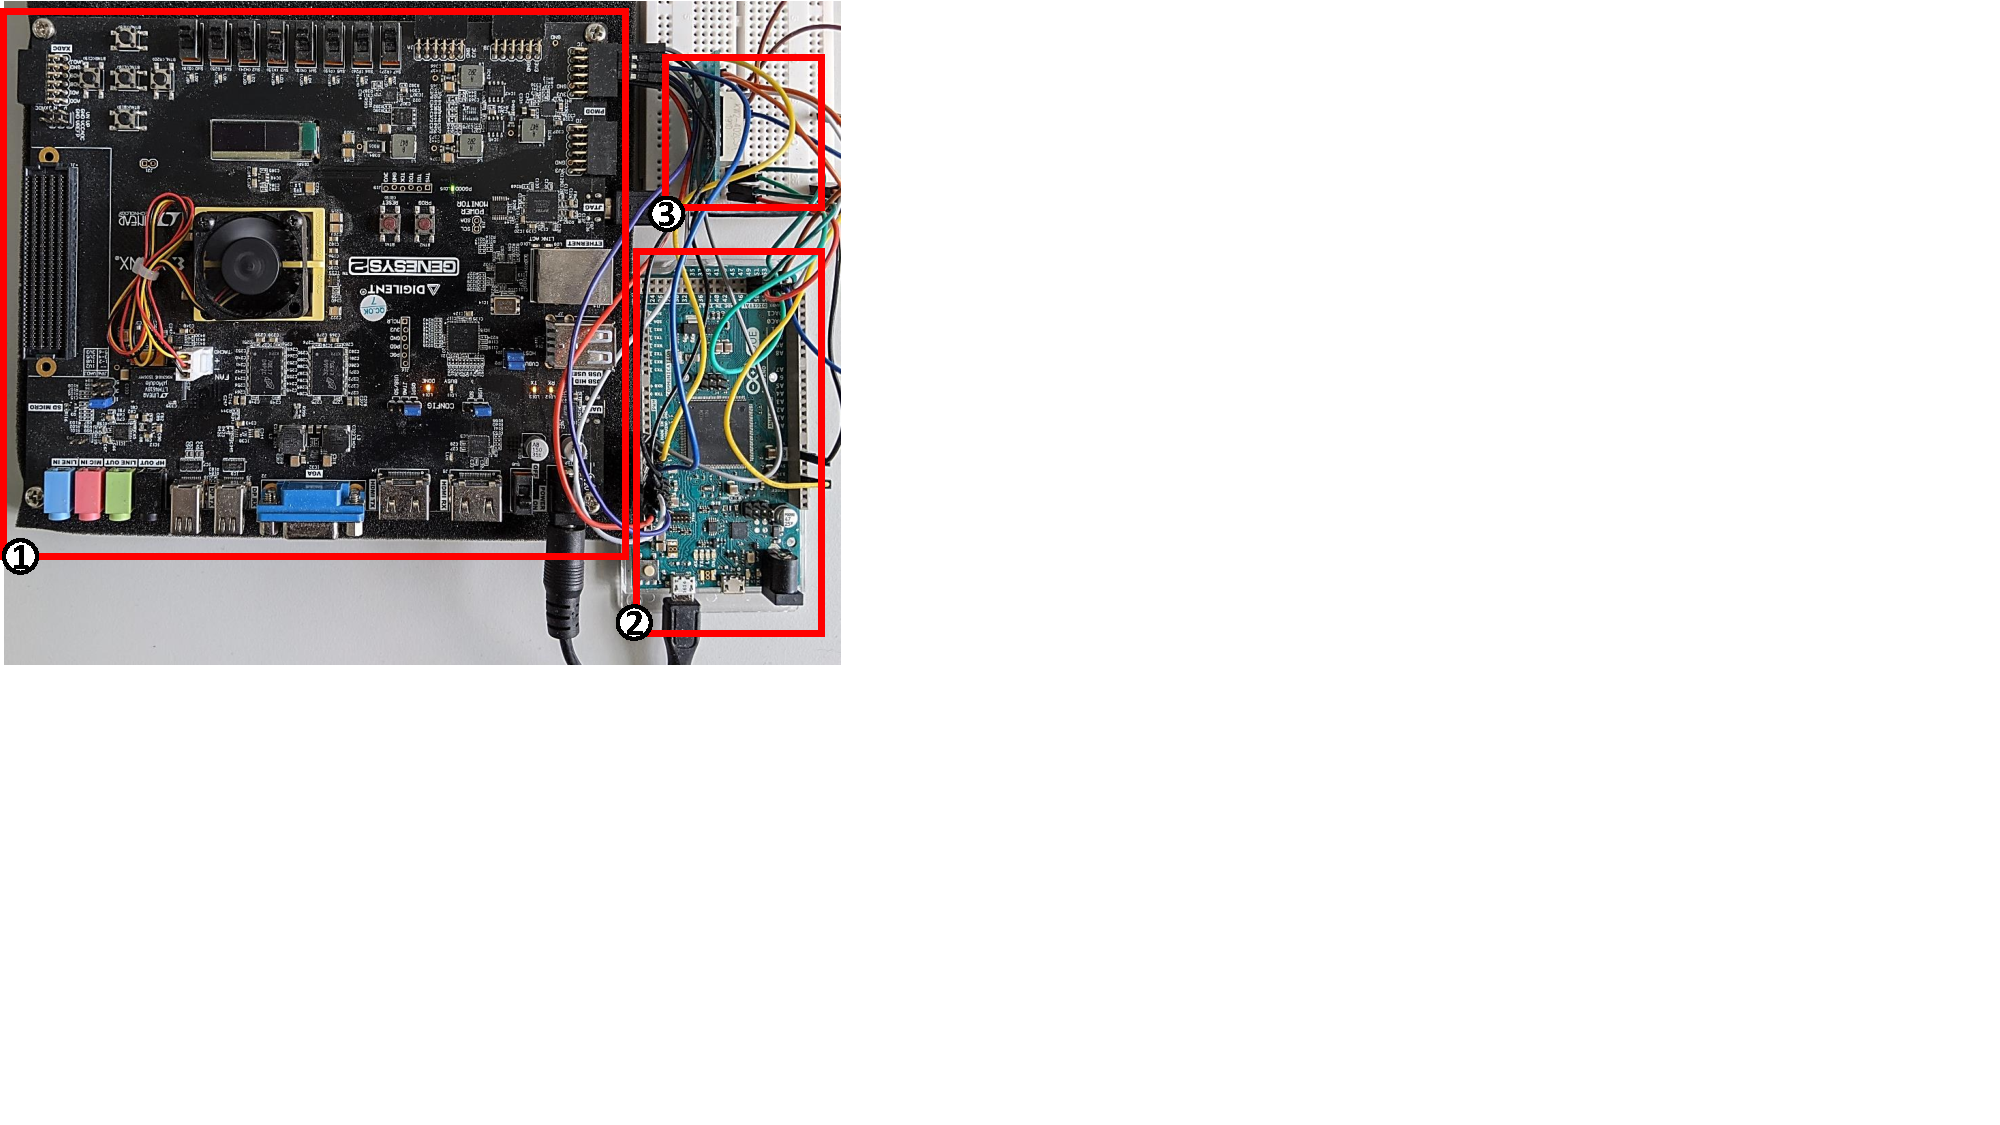
\includegraphics[trim={0 8cm 19cm 0}, clip, width=0.9\linewidth]{chapters/PIE/images/prototype.pdf}
\caption[\name prototype]{The figure shows different components of our prototype: \one Digilent Genesys 2 FPGA board, \two Arduino Due as the peripheral simulator, and \three a seven-segment display unit as an example peripheral.} %\vspace{-2em}
\label{fig:prototype}
\end{figure}

\subsection{Implementation}
\subsubsection{FPGA prototype}
\label{sec:eval:prototype}
We implemented an end-to-end prototype of \name that is based on the Keystone enclave framework~\cite{keystone}. Figure~\ref{fig:prototype} shows a case study on a platform that consists of an FPGA emulating the central processor connected to several Arduino boards that emulate \sphw. %We also discuss the added complexity in the form of trusted computing base of our prototype. Since added complexity is hard to quantify, we fall back on the metric ``lines of code'' for the TCB. 

\paragraph{FPGA platform}
We base our system on the Ariane core~\cite{ariane}, an open-source RISC-V 64-bit core that supports commodity OS such as Linux. It is an RC64GC 6-stage application class core that has been taped out multiple times and can operate up to 1.5 GHz. We run this core on a Digilent Genesys 2 FPGA board (\one in~\Cref{fig:prototype}).

We added PMP capability to the core that originally does not support PMP using 160 lines of SystemVerilog. The PMP unit is formally verified against a handwritten specification with yosys~\cite{wolf2016yosys}. Two of these units are inserted into the memory management unit (MMU) and are responsible for checking data accesses and instruction fetches. An additional unit is placed in the hardware page table walker to check page table accesses.
Our implementation has a configurable number of PMP entries up to the maximum number of 16 mandated by the standard~\cite{riscv2019privspec}. Our modifications have been contributed to the Ariane project and are open source~\cite{arianegithub}. Note that PMP is part of the RISC-V privilege standard and as such is already available on many other cores~\cite{asanovic2016rocket,ibex}. 

\paragraph{Processor-local enclaves}
%\name prototype leverages Keystone enclave framework~\cite{keystone} that uses a low-level trusted security monitor to run enclaves. 
We modified the SM to be able to connect two enclaves or an enclave and \sphw. Specifically, we added three new interfaces to the SM called \texttt{connect}, \texttt{sync\_disconnect}, and \texttt{async\_disconnect}. These interfaces can be used to set up shared regions between two enclaves or \sphw specified by their identifier. We also modified Keystone's attestation procedure to include a list of identifiers for all connected enclaves. Our modifications only amount to 390 additional or modified lines of code. The SM consists of around 2000 lines of code excluding SHA3 and ed25519 implementations that contribute around 4000 additional lines of code. %Our extension thus amounts to 9\% of added lines of code to Keystone (and 4.5\% including the crypto libraries).

In Keystone, every enclave runs on top of a minimal runtime that handles syscalls and manages virtual memory. Hence, its code is critical and part of the TCB. For our prototype, we added support to dynamically map shared memory regions into the virtual address space of an enclave. We modified 213 LoC out of a total of 3600 LoC for Keystone's runtime.

On the untrusted OS side, there are many components to make it easier to create and run enclaves such as an SDK and a kernel driver. These components also required numerous changes. However, they are not trusted and as such do not increase the TCB. 

\paragraph{Simple \sphw}  In our prototype, we emulated the a number of simple \sphw (e.g., keyboard, mice, simple sensors, etc.) on the Arduino Due microcontroller prototyping board (\two in Figure~\ref{fig:prototype}) using Arduino HID library. The Due's GPIO pins are connected to the FPGA's PMOD pins over two pairs of $8$ wires for bi-directioanl data. We modify the $I^2C$ protocol to communicate data between the Due and the FPGA. The physical limitations of the PMOD pins restricts the channel's frequency to $8$ MHz yielding 1 MB/s bandwidth. In the real world, the physical interfaces between the \sphw and the platform could be diverse such as USB, PCI-E, etc. As a concrete example, we implemented a keyboard with the Arduino board and wrote a simple keyboard driver that interprets the GPIO signal from the Arduino. Additionally, we use a PMOD interface-based seven-segment display unit as an output peripheral (\three in Figure~\ref{fig:prototype}). The driver contains around 50 LoC and is incorporated into our example controller enclave. Additionally, we use the \texttt{USBHost} library that can emulate a number of USB peripheral devices on the Arduino. We use the Arduino cryptographic library for signing the challenge messages from the \ce during the local attestation. The Due uses 128-bit AES (CTR mode) for encryption, HMAC\_SHA256 for message authentication, Curve25519 for key exchange, and SHA3 for the hash function. We use \texttt{DueFlashStorage} library to implement the NVM flash that contains the key materials for the peripheral attestation. Our prototype implementation is approximately 2.5K lines of code.

\subsubsection{Accelerator}
\label{sec:eval:accel}

We conduct another case study to show how complex \sphw such as a GPU-scale accelerator~\cite{zaruba2020manticore} can be extended to support \name. The accelerator is a 4096-core RISC-V platform that has comparable performance to current state-of-the-art machine learning accelerators. It is organized in clusters each with 8 individual single-stage RISC-V cores~\cite{zaruba2020snitch}, each of which is accompanied by a double precision floating point unit capable of two double precision and four single precision flops per cycle. To hide memory latency, all clusters have access to a scratchpad memory and a large L2 data cache. 

To provide multi-tenant isolation on the accelerator, we introduce a shared PMP unit with 4 entries into every cluster. The PMP entries can only be configured by one out of eight cores but the access policies will be enforced on all of them. With this additional hardware support we were able to implement a small firmware that configures the PMP entries according to the specifications from the host and then runs a task in user mode. Upon a context switch, the scratchpad memory that was in use by the previous task must be flushed and the PMP entries must be reconfigured. The firmware consists of 143 lines of assembly and 73 lines of C code. This implementation and verification takes around 3 weeks.

\subsection{Performance}
\label{sec:eval:numbers}
We list \name{}'s performance in the following categories:

\setcounter{para}{0}

\mypara{Performance of enclave communication}
%A comparison between traditional enclave communication and our shared memory model is quite pointless. 
Since \name{} supports shared memory to communicate, its communication speed is the same as what the memory bus provides. This is much faster compared to traditional TEEs, where enclaves communicate through the OS requiring extra encryption steps. Concurrent work also demonstrates the performance gains that can be extracted from enclave to enclave communication using shared memory~\cite{yu2020elasticlave}.

% In traditional TEEs, the enclaves communicate through the untrusted operating system. Therefore, they first have to perform local attestation to establish a shared key which is then used to encrypt every message. Contrary to traditional TEEs, in \name, the enclaves establish a shared memory region to communicate directly. Hence, they do not need to encrypt messages as only the communicating enclaves have access to that shared memory. The shared memory enables the communication between enclaves to achieve the same performance what the memory bus could provide. 
% %This also requires some work by the SM similar to the local attestation for traditional enclaves. Thus, one approach requires encryption and the other does not. Since our platform does not support any kind of hardware acceleration for encryption algorithms, the performance difference between the two approaches would be huge. Therefore, we do not believe a comparison between these two systems is meaningful. 
% Recent work also shows the performance gains that can be extracted from enclave to enclave communication using shared memory~\cite{yu2020elasticlave}.

\begin{figure}[t]
    \centering
    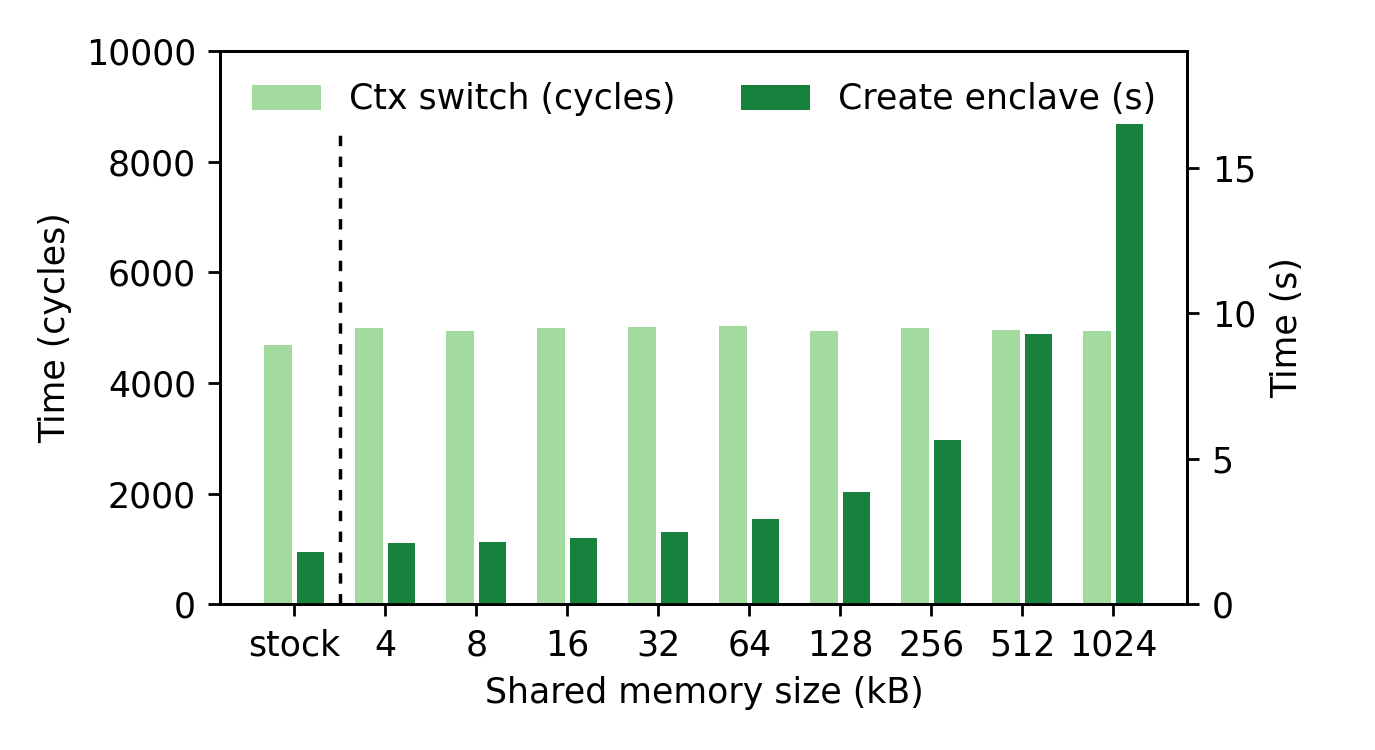
\includegraphics[width=\linewidth]{chapters/PIE/images/graphs/ctxswitch.png}
    \vspace{-3em}
    \caption[Context switch performance]{Context switch performance for varying sizes of a shared memory region compared to stock Keystone performance on the left (equivalent to no shared memory).}
    \label{fig:ctxswitches}
\end{figure}

\mypara{Context switches}
Context switches are critical for any system and determine its responsiveness and a part of its performance.
We performed experiments for various sizes of shared memory region and gathered various context switch latencies in \Cref{fig:ctxswitches}. We also measured the time of enclave creation which is mostly dominated by copying all the enclave data from the untrusted OS to the protected memory region and thus is expected to be linear in terms of shared memory size. 

These measurements highlight that the context switches are independent on the shared memory size. The absolute context switch time increases from 4730 for stock Keystone to 4950 for \name{}.
% We report that the performance within an enclave in our prototype is equivalent to the performance of stock Keystone~\cite{keystone}. This is reasonable since we do not modify anything that would affect Keystones performance.

\mypara{PMP overhead}
We measure the hardware overhead of PMP units in terms of the logic, the caches, and the total amount in NAND2 gate equivalents within the processor pipeline for 0, 8, and 16 PMP entries, and present them in \Cref{tab:eval:ariane}. We instantiate the Ariane core~\cite{ariane} with the default configuration: including the floating point unit, 32KiB L1 data cache, 16KiB L1 instruction cache, branch history table of size 64, and a 16-entry branch target buffer. We synthesized this instantiation of the core in a 22nm technology at 1GHz. %In order to provide a meaningful comparison, we provide the separate size of the logic, the caches, and the total amount in NAND2 gate equivalents in \Cref{tab:eval:ariane}. 

\begin{table}[tbp]
    \centering
    \caption{Size of the default configuration of the Ariane core in gate equivalents (GE), synthesized in 22nm at 1GHz with varying number of PMP entries.}\vspace{-0.5em}
    \begin{tabular}{llll}\toprule
        PMP entries & logic & caches & total \\\midrule
        0 & 472k GE & 686k GE & 1141k GE \\
        8 & 497k GE & 686k GE & 1164k GE \\
        16 & 531k GE & 686k GE & 1197k GE \\ \bottomrule
        % Overhead & 12.4\% & 0\% & 4.9\% \\ \bottomrule
    \end{tabular}
    
    \label{tab:eval:ariane}
\end{table}

\mypara{Simple \sphw} The communication overhead between the platform and the peripheral device emulated by the Arduino due is very small. At the time of initialization, the peripheral and the platform exchanges handshake messages to perform local attestation. The initial handshake message is $60$ bytes. Every message size of our modified $I^2C$ protocol is 32 bytes. The combined latency introduced by signing averages around 60 $\mu$s.

\mypara{Accelerator}
Our modification of the accelerator cores increases size by around 15\% and slows down from 750MHz to 666MHz due to the impact of the PMP access checks on the critical path. Note that this may not reflect the general case but rather reflects an upperbound. The change in area of a single core complex (core, FPU, and an integer subsystem) can be found in \Cref{fig:areasnitch}. In total, the area of the entire accelerator only increased by around 0.6\%, with most of the area being occupied by the floating point units.
%The implementation and verification of the firmware took another engineering week. 


\begin{figure}
    \centering
    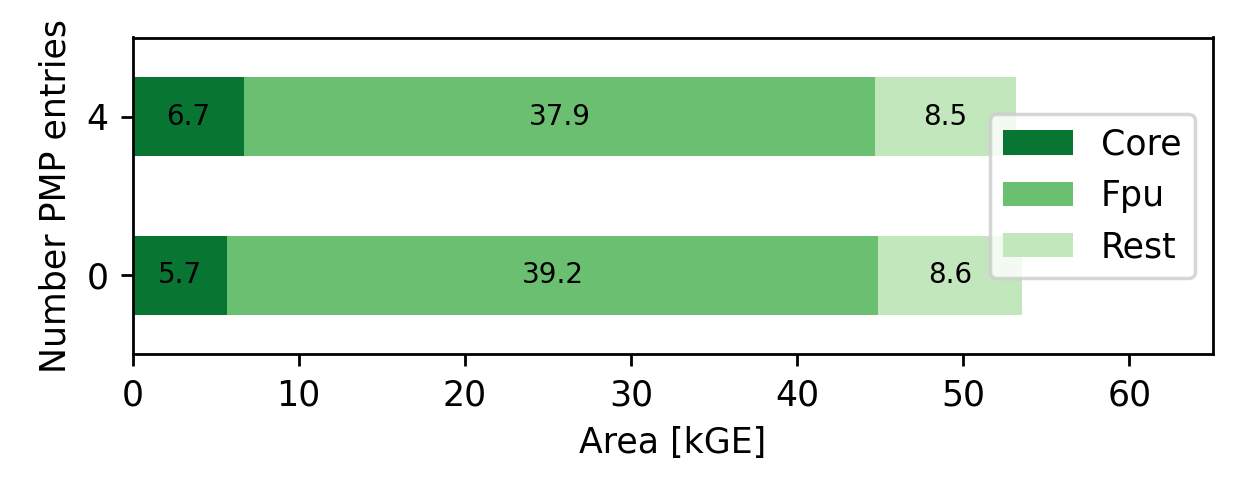
\includegraphics[width=0.9\linewidth]{chapters/PIE/images/graphs/areasnitch.png}
    \vspace{-1em}
    \caption[The post-synthesis area of a core complex of our accelerators]{The post-synthesis area of a core complex of our accelerators, with four and zero PMP entries respectively. Note that the design was synthesized with 750MHz clock for 0 PMP entries and 666MHz with 4 entries. The size of the core increases due to the increased pressure by the PMPs, while the FPU gets smaller with the lower clock as its critical path is not affected by the PMP entries.}
    \label{fig:areasnitch}
\end{figure}

\setcounter{para}{0}





\section{Discussion} 
\label{integriscreen:sec:discussion}

% We now discuss open questions, limitations, and possible extensions.

\myparagraph{Detecting user attention and non-repudiation}
In this chapter, the system uses hand movement to detect user's presence and activity.
However, when the mobile device is placed between the host and the user, its front facing camera is well positioned to capture the user's face.
Given the face tracking capabilities available in recent iOS and Android mobile phones, as well as recent advances in mobile camera-based eye tracking~\cite{krafka2016eye}, the system could be extended to precisely track user's attention on the screen and require that gaze is present for certain data modification.
Furthermore, if the mobile device used face recognition to continuously authenticate the user, the system could also provide non-repudiation guarantees.


\myparagraph{Non-textual UI elements}
As the first of the proposed \textit{visual supervision} paradigm, in this chapter, we focused on textual input.
However, our approach can be extended to support non-textual UI elements -- as long as their final state is shown on the screen -- such as checkboxes, sliders, or calendar widgets.
Furthermore, while we focused on text extraction, this step could be implemented by a more literal comparison of the host's screen with a screenshot of the web form, as rendered by the server with same aspect ratio and element position.

\myparagraph{Privacy and security of visual supervision}
While continuously recording one's interaction with another electronic device seems intrusive, we note that all processing in \sysname happens on the mobile device.
Therefore, the server only receives a duplicate of the data from the host.
If sending a duplicate of the data is not suitable for any reason, it is straightforward to modify \name to compute and only send a digest (similar to a TAN) to the server.

However, a visual channel gives users clear control over which data the mobile device observes, i.e., only what is shown on the screen at a given moment -- while most OS level applications typically get unrestricted access to the whole system and could violate the users' privacy in the background while keeping them oblivious.

Finally, using only a visual channel between the host and the mobile device reduces the likelihood of a smartphone compromise, since it never directly communicates with the already compromised host.
\section{Related Work}
\label{sec:relatedWork}

In this section, we discuss some of the most relevant works to \name. We also discuss the main differences with \name to these works.


\subsection{TEE-based solutions}
There exist several solutions for integrating external devices to widely deployed TEEs: Intel SGX, and ARM TrustZone. 

\myparagraph{SGXIO} SGXIO is a proposal by Weiser et al.~\cite{weiser2017sgxio} that builds on top of Intel SGX, intending to allow SGX to interact with input-output devices. They achieve that by introducing a trusted hypervisor that allows enclaves to access virtualized peripherals. Similar to our approach, SGXIO also considers a remote adversary. However, SGXIO is rather static in nature, i.e., all the peripherals have to be set up at boot time. After the system setup phase, no changes are allowed (connect new peripherals, etc.). It is not clear how enclaves are created and get access to a peripheral while preserving the confidentiality of previous enclaves that used said peripheral. Essentially, SGXIO allows for a static extension of the hardware TCB.

\myparagraph{Graviton and systems based on it} Graviton~\cite{volos2018graviton} is a TEE that runs on an accelerator such as a graphics card. It can provide isolation between the data of multiple stakeholders that run tasks on the GPU concurrently. It also provides remote attestation of an enclave on the accelerator. Graviton was evaluated on a modern graphics card and shows that the predominant overhead stems from encryption of the communication to the processor. However, they also demonstrate that the overhead of around 20\% is tolerable. Graviton would fit very well within a \name{} as it is an excellent example of an enclave on a peripheral. It provides isolation for secret data and attestation reports. In addition, it shows that even some of the most powerful accelerators can be extended with a local TEE. Visor~\cite{visor} is a system built upon Graviton~\cite{volos2018graviton} that proposes a hybrid TEE that spans over both CPU and GPU. Visor is aimed towards privacy-preserving video analytics where the computation pipeline is shared between the CPU (non-CNN workloads) and the GPU (CNN workloads) to increase efficiency. Visor addresses micro-architectural-based side-channel attacks where a local physical attacker can use the data-dependent memory access patterns (e.g., branch-prediction, cache-timing, or controlled page fault attacks) to reveal elements on the video analysis (e.g., leaks pixel patterns). The communication between the CPU and GPU enclaves is encrypted. Additionally, Visor ensures that the traffic pattern between the CPU and GPU enclaves is independent of the video content.

\myparagraph{HETEE} HETEE~\cite{zhu2020hetee} is another proposal to extend TEEs to accelerators (specifically GPUs) without requiring changes to existing CPUs/GPUs. HETEE focuses on data center applications and proposes an extra hardware box per rack that is protected from physical attacks. This box also contains all accelerators, which it then connects to compute servers in the same rack. Each enclave then runs on a dedicated compute server and a connected accelerator. In essence, the HETEE box provides secure routing of accelerators to dedicated compute servers. In contrast to HETEE, we aim to be able to execute multiple composite enclaves on the same compute server. 


\myparagraph{ARM TrustZone and systems based on it} TrustZone is a system TEE provided by ARM for their system-on-chips (SoC)~\cite{winter2008trusted}. TrustZone applications run on top of a secure OS that is trusted and isolated from the standard operating system (also known as the rich OS). Isolation between the two worlds is achieved by an extra bit on the bus. 
%and some additional configurable components such as the TrustZone Address Space Controller (AZASC). The AZASC is a dedicated hardware component on the SoC that may permit and refuse some access to memory. 
However, there is no isolation between different TrustZone applications. Due to this limitation, mobile phone manufacturers usually only allow TrustZone applications that are signed by them. % --  a restricted version of the local attestation. 
TrustZone only provides the lower level isolation property between the rich OS and the secure OS. Everything else, i.e., isolation between TrustZone applications, remote attestation, etc., has to be added to the secure OS~\cite{ning2014samsungknox}. There have been many proposals that try to improve on the capabilities of TrustZone~\cite{brasser2019sanctuary,hua2017vtz}. Sanctuary~\cite{brasser2019sanctuary} enables user-space TrustZone enclaves. Sanctuary achieves isolation by running enclaves in their own address space in the normal world. However, Sanctuary is very similar to Intel SGX, and thus, it does not extend to peripherals.
%Similar to these proposals, TrustZone could also be extended in the direction of \name{} to support \nameenclave{}s. 
There exist proposals that enable additional security properties such as a trusted path by enabling direct pairing of peripherals (e.g., the touchscreen) to the TrustZone application. Such proposals include TruZ-Droid~\cite{TruZ-Droid}, TrustUI~\cite{trustUI}, SeCloak~\cite{SeCloak}, VButton~\cite{VButton}. All of these solutions do not provide any form of peripheral attestation similar to \name{}. They also do not consider other peripherals or how to dynamically allow an enclave to access a peripheral previously used by another enclave. Moreover, as mentioned earlier, the absence of isolation between the TrustZone applications makes the proposal mentioned above weak in inter enclave isolation guarantee.


\subsection{Other isolation methods} 

Minimal hypervisors or operating systems~\cite{herder2006minix,klein2009sel4} can also achieve isolation, and some are even formally verified~\cite{klein2009sel4}. Usually, such hypervisors do not include attestation, but the cost of adding that should be very low. A \name{} could also be based on a microkernel such as seL4. One would have to add an interface for the malicious OS running in a virtual machine to interact with enclaves that run directly on top of seL4, similar to other pure hypervisor-based isolation systems~\cite{virtualGhost,Overshadow,InkTag,TrustVisor,SplittingInterfaces,terra}. It might even be possible to formally prove such modifications to provide an even stronger assurance of isolation. Similar to other pure hypervisor-based isolation system include Virtual Ghost~\cite{virtualGhost}, Overshadow~\cite{Overshadow}, InkTag~\cite{InkTag}, TrustVisor~\cite{TrustVisor}, Splitting Interface~\cite{SplittingInterfaces}, Terra~\cite{terra} etc.  The hypervisor is also in charge of the scheduling, resulting in a significantly bigger TCB than \name. Moreover, in none of the hypervisor-based proposals, platform awareness and platform-wide attestation are considered. Isolation is the sole objective of these proposals.

\subsection{Bump in the wire-based solutions} 

Fidelius~\cite{Fidelius}, ProtectIOn (refer to Chapter~\ref{ch:protectIOn}), IntegriScreen (refer to Chapter~\ref{ch:integriscreen}), FPGA-based overlays~\cite{fpga_overlay}, IntegriKey (refer to Chapter~\ref{ch:integrikey}) are some of the trusted path solutions that use external trusted hardware devices as intermediaries between the platform and IO devices. These external devices create a trusted path between a remote user and the peripheral and enable the user to exchange sensitive data securely with the peripheral in the presence of an attacker-controlled OS. Such solutions provide a loose notion of platform awareness and are focused on IO devices. Platform-wide attestation and strong isolation guarantee are out-of-scope of such proposals. 



% \begin{table*}[t]
%   \centering
%   \resizebox{\textwidth}{!}{%
%     
\newcommand{\yes}{\CIRCLE}
\newcommand{\no}{\Circle}
\newcommand{\yesno}{\LEFTcircle}
% \newcolumntype{Y}{>{\centering\arraybackslash}X}
\begin{tabular}{@{}lcccccccccccccccc@{}}
% \begin{tabularx}{\textwidth}{@{}lcclclYYYlYYYlYYY@{}}
% \footnotesize
% \begin{tabular}{@{}lcccccccccccccccc@{}}
\toprule
    & \multicolumn{4}{c}{Platform Awareness} &  & \multicolumn{11}{c}{Isolation between Partitions} \\ \cmidrule(lr){2-5} \cmidrule(l){7-17} 
    & \multicolumn{2}{c}{Attestation} &  & \multirow[c]{2}{*}[-3pt]{\begin{tabular}[c]{@{}l@{}}Bidirectional\\ Awareness\end{tabular}} &  & \multicolumn{3}{c}{Spatial} &  & \multicolumn{3}{c}{Temporal} &  & \multicolumn{3}{c}{Fault} \\ \cmidrule(lr){2-3} \cmidrule(lr){7-9} \cmidrule(lr){11-13} \cmidrule(l){15-17} 
    & Enclave & Platform &  &  &  & \multicolumn{3}{c}{Core/SoC/Platform} &  & \multicolumn{3}{c}{Core/SoC/Platform} &  & \multicolumn{3}{c}{Core/SoC/Platform} \\ \midrule
SGX~\cite{costan2016intel} & \yes & \no &  & \no &  & \yes & \no & \no &  & \no & \no & \no &  & \yes & \yes & \no \\
Sanctum~\cite{costan2016sanctum} & \yes & \no &  & \no &  & \yes & \no & \no &  & \yes & \yes & \no &  & \yes & \yes & \no \\
Keystone~\cite{keystone} & \yes & \no &  & \no &  & \yes & \no & \no &  & \yesno & \yesno & \no &  & \yes & \yes & \no \\
Sancus~\cite{noorman2013sancus} & \yes & \no &  & \no &  & \yes & ? & \no &  & \no & \no & \no &  & \yes & ? & \no \\
TrustZone & ? & \no &  & \no &  & \yesno & \yesno & \no &  & \no & \no & \no &  & \no & \no & \no \\
Samsung Knox & \yes & \no &  & \no &  & \yesno & \yesno & \no &  & \no & \no & \no &  & \no & \no & \no \\
Sanctuary~\cite{brasser2019sanctuary} & \yes & \no &  & \no &  & \yes & \no & \no &  & \no & \no & \no &  & \yes & ? & \no \\
TPM & ? & \no &  & \no &  & \no & \no & \no &  & \no & \no & \no &  & \no & \no & \no \\
DRTM & \yes & \no &  & \no &  & \no & \no & \no &  & \no & \no & \no &  & \no & \no & \no \\
XOM~\cite{lie2000xom} & \yes & \no &  & \no &  & \no & \no & \no &  & \no & \no & \no &  & \no & \no & \no \\
Aegis~\cite{suh2003aegis} & \yes & \no &  & \no &  & \yes & \no & \no &  & ? & ? & \no &  & ? & ? & \no \\
% Bastion & \yes & \no &  & \no &  & \yes & \no & \no &  & ? & ? & \no &  & ? & ? & \no \\ \bottomrule
% \end{tabularx}
\end{tabular}
%   }
%   \caption{Comparison between traditional TEEs.\todo{Fill remaining question marks. Add daggers for all isolation facilitated by MMU}\todo{Change to the new requirements}}
%   \label{tab:comparison}
% \end{table*}


\section{Conclusion} 
\label{integriscreen:sec:conclusion}

In this chapter, we explore the idea of \emph{visually supervising} user's IO data to provide IO integrity against a compromised host. We use a smartphone to capture the client's screen and enforce the integrity of the web rendered on the screen, alongside the input data the user submits on the web form. We show the feasibility of this approach by developing a fully functional prototype on an Android smartphone, evaluating it with a series of experimental tests, and running a user study to measure participants' responses to simulated attacks.
Considering the rapid increase in processing power and camera quality of smartphones, but also novel platforms such as augmented reality headsets and smart home assistants, we envision such systems that supervise user's IO will be ubiquitous.


%\bibliographystyle{IEEEtranS}
\bibliographystyle{ACM-Reference-Format}
\bibliography{bibliography} 

%\appendix
%\subsection{Proof for IO Integrity}
\label{appendix:security}

In this appendix, we provide a formal proof of the following property: \emph{without protecting both input and output integrity, none of them can be achieved}. 


%\subsection{Interaction Protocol} 
%\label{appendix:security:protocol}

\myparagraph{Interaction protocol}
To simplify the proof, we model the interaction between the user, the host, and the remote server as a finite state automaton (FSA).
The interactions between the server (\server), the user (\user) and host (\host) are depicted in the FSA in Figure~\ref{fig:fsm}.

\begin{figure}[h!]
\begin{center}
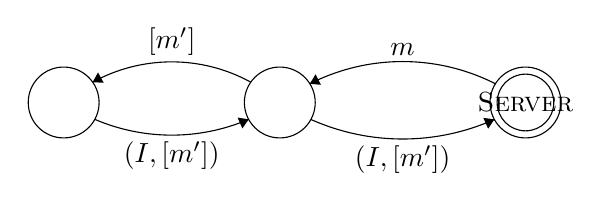
\begin{tikzpicture}[scale=0.15]
\tikzstyle{every node}+=[inner sep=0pt]
\draw [black] (66,-23.1) circle (3);
\draw (66,-23.1) node {\server};
\draw [black] (66,-23.1) circle (2.4);
\draw [black] (45.2,-23.1) circle (3);
\draw (45.2,-23.1) node {\host};
\draw [black] (26.9,-23.1) circle (3);
\draw (26.9,-23.1) node {\user};
\draw [black] (47.743,-21.516) arc (116.95563:63.04437:17.332);
\fill [black] (47.74,-21.52) -- (48.68,-21.6) -- (48.23,-20.71);
\draw (55.6,-19.13) node [above] {$m$};
\draw [black] (29.352,-21.382) arc (118.8302:61.1698:13.89);
\fill [black] (29.35,-21.38) -- (30.29,-21.43) -- (29.81,-20.56);
\draw (36.05,-19.16) node [above] {$[m']$};
\draw [black] (42.565,-24.526) arc (-66.78269:-113.21731:16.527);
\fill [black] (42.57,-24.53) -- (41.63,-24.38) -- (42.03,-25.3);
\draw (36.05,-26.36) node [below] {$(I,[m'])$};
\draw [black] (63.369,-24.535) arc (-65.91058:-114.08942:19.034);
\fill [black] (63.37,-24.53) -- (62.43,-24.4) -- (62.84,-25.32);
\draw (55.6,-26.69) node [below] {$(I,[m'])$};
\end{tikzpicture}
\end{center}
\caption{Finite state machine that depicts the interaction between the user (\user), host (\host) and the server (\server).}
\label{fig:fsm}
\end{figure}

\server sends a message $m$ to \host. One can assume $m$ to be the HTML, JavaScript, and other data send from \server as a HTTP response. We denote $[m]$ to be the render of $m$ by the \host. As \host is malicious, it can transform $m$ to $m'$. Note that the transformation is public knowledge and is deterministic. If $m\neq m'$ then given $[m]$ and $[m']$, \server can determine that $[m]\neq [m']$. We denote the user input to be $I$, which corresponds to a specific $[m]$. 
%Note that the communication channel between \server to \user is neither authenticated, neither confidential. But the communication channel from \user and \server is authenticated. 
In this model, we simplify the user input by assuming that the \user only provides an input $I$ only after observing a message transformation $[m]$. The user provides both her input $I$ and transformation $[m']$ observed by her to \host. The interaction loop between \host and \user can continue until \user finishes her input. After every input \host hands over new message transformation to \user (either result of the input or new message from \server or both). Once the user provides all her inputs, \host send the pairs $(I, [m'])$ to \server.

We also define two mappings:
\begin{align*}
\texttt{Input()}&:[m]\rightarrow I \\
\texttt{Transform()}&:m,I\rightarrow [m'],\ \exists i\in I:i=\phi
\end{align*}
Both of them are \emph{bijective}.

One trace of the protocol transcript is depicted in Figure~\ref{fig:protocol}. As described in the FSM, \server receives traces of message transformation ($[m']_1,[m']_2,\ldots,[m']_n$) and corresponding inputs ($I_1,I_2,\ldots,I_n$). From these traces \server could determine of all the $[m']_i$ are in proper form by verifying if $[m]_i=[m']_i$.

\begin{figure}[t]
\begin{center}
\tikzset{
  every picture/.append style={
    transform shape,
    scale=0.8
  }
 }
\begin{sequencediagram}
\newinst{u}{\user}
\newinst[3]{h}{\host}
\newinst[3]{s}{\server}
\mess{s}{$m$}{h}
\mess{h}{$[m']_1$}{u}
\mess{u}{$I_1,[m']_1$}{h}
%\mess{h}{$[m']_2$}{u}
%\mess{u}{$I_2,[m']_2$}{h}
\mess{h}{...}{u}
\mess{u}{...}{h}
\mess{h}{$[m']_n$}{u}
\mess{u}{$I_n,[m']_n$}{h}
\mess{h}{$I_1,I_2,...,I_n$}{s}
\mess{h}{$[m']_1,[m']_2,...,[m']_n$}{s}
\end{sequencediagram}
\end{center}
\caption{Protocol transcript between the \server, \user and \host that shows one trace from the FSM depicted in Figure~\ref{fig:fsm}.}
\label{fig:protocol}
\end{figure}


\begin{definition}{\textbf{Input integrity}}
\label{def:inputIntegrity}
Assume that \server handed a message $m$ to \host where the proper message transformation is $[m]$. The host changes the message transformation to $[m']$ where $[m']\neq [m]$. We also define correct \user input to be $I$ when \host sends a correct message transformation $[m]$ to \user. We define input integrity as the property where the \server does not accept input $I'$ where $I'\neq I$from \user if the \host changes the message transformation.
\end{definition}

\begin{definition}{\textbf{Output integrity}}
\label{def:outputIntegrity}
Assume that \server handed a message $m$ to \host where the proper message transformation is $[m]$. Output integrity defines that in all circumstances, \user receives the correct message transformation $[m]$ from \host.
\end{definition}

\myparagraph{Verification process} \server checks $\forall i=1\ldots n$ $$[m']_i = \texttt{Transform}(m_{i-1}, I_{i-1})$$ where $I_0=\phi$.

\begin{theorem}
\label{theorem:th1}
If \user does not send all the transformations till $[m']_i$ corresponding to the input $I_i$, input integrity can not be achieved. 
\end{theorem}

\begin{IEEEproof}
If \user does not attach all the transformation till $[m']_i$, i.e., $[m']_1, [m']_2, \ldots, [m']_{i-1}, [m']_i$  corresponding to inputs $I_1, I_2,\ldots, I_{i-1}, I_i$, then the server can not verify all the transformations corresponding to the input. \host could modify a specific $[m]_x$ to influence \user input.
\end{IEEEproof}

\begin{theorem}
\label{theorem:th2}
If the channel from \user and \server is not authenticated, input integrity is not achievable. But the channel from \server to \user does not require to be secure as long a \user provides the message transformation $[m']_i$ corresponding to every input $I_i$.
\end{theorem}

\begin{IEEEproof}
The proof is trivial. If the channel from \user to \server is not authenticated, any input provided by \user can be manipulated by \host without a trace. Hence input integrity is not achievable. As long as \user sends message transformation along with the input, a manipulated message transformation bt \host would be detectable by \server (see Theorem~\ref{theorem:th1}).
\end{IEEEproof}

\begin{theorem}
\label{theorem:th3}
Ensuring output integrity also ensures input integrity provided there is an authenticated channel from \user to \server.
\end{theorem}

\begin{IEEEproof}
This proof is also trivial. As we describe in the Definition~\ref{def:inputIntegrity} and~\ref{def:outputIntegrity}, if all the message transform from \host $[m']=[m]$, and \host always executes \texttt{transform()} properly, the input integrity is preserved. As \name ensures output integrity and all the input from the user is signed by the \device, \name preserves input integrity. 
\end{IEEEproof}


%\section*{Implementation Details}
%\label{appendix:implementation}

\subsection{Implementation of \name Components}
\label{appendix:implementation}


In the following, we provide the implementation details of the \name components presented in the previous sections. 

\myparagraph{QR code generation \& UI specification}
\label{sec:prototype:impl:qr}
%
QR code generation phase is executed by \name JS that transforms the UI elements of a sensitive web form to a UI specification encoded in a QR code (we use QRCode.js, a \js library to produce QR codes). Section~\ref{sec:systemDesign:transformation} provides the high-level concept of generating the QR code from the webpage UI elements. UI elements that require IO integrity protection can be marked by the developers in the \html source. As illustrated in Figure~\ref{fig:transformation}, the \html UI elements: `\texttt{Sensitive field 1}' and `\texttt{Sensitive field 2}' have the additional attribute \texttt{protect=``true''}. %(one concrete example is illustrated in Figure~\ref{fig:transformation}). 

The \name JS iterates through the HTML elements that have the \texttt{protect} attribute enabled and extracts the information such as the name of the label or the type of the UI element. \device uses preloaded size parameters to specify the size of a text field, button, etc. in case the size is not explicitly mentioned in the HTML source. One important attribute for a UI element in the specification is the \texttt{trigger}. For example, in Specification~\ref{snippet:UISpecification}, the \texttt{OK} and the \texttt{cancel} buttons have an attribute \texttt{trigger}. This attribute is Boolean can be either \texttt{true} (corresponding to \texttt{OK}) or \texttt{false} (corresponding to \texttt{Cancel}) value. The value \texttt{true} denotes that the \texttt{OK} button can submit the values that are provided by the user. The \texttt{false} attribute denotes that hitting the \texttt{cancel} button abort the form altogether. 

The QR code generation phase is between \one and \two in Figure~\ref{fig:transformation} where the \name JavaScript snippet transforms the UI elements to a UI specification language in a QR code that can be interpreted by the \device. The UI specification corresponding to the \html source (in Figure~\ref{fig:transformation}) is provided in Specification~\ref{snippet:UISpecification}. Note that the specification is highly flexible, allowing adjustable size for the form, individual UI elements, gaps between them, etc. This allows the \device to faithfully recreate the UI that is very close to the actual form UI that the served by the web severer. 
%Such allows negligible user habituation. 

\myparagraph{Bitmap generation}
\label{sec:prototype:impl:bitmap}
%
The \device reads the QR code from the HDMI frame and generate the UI overlay bitmap from it. We have used the \texttt{piCamera} library to intercept the HDMI frames and generate the UI on top of it. Our \name prototype implements the most frequently used HTML input elements~\cite{html_elements} that are common in sensitive forms. 

\myparagraph{Detection of mouse pointer}
\label{sec:prototype:impl:mouse}
%
Initially, when the system boots up the \device perform the calibration phase (see Section \ref{sec:systemDesign:analysis:calibration}) to synchronize its coordinates of the pointer with the host. The detection of the mouse pointer is implanted partially on the raspberry pi 4 (\six in Figure~\ref{fig:prototypeAll}), while the mouse intercepting is done in the Arduino Due (\three in Figure~\ref{fig:prototypeAll}). The Due gathers the raw mouse data (in terms of displacement measurements $(\Delta x_i, \Delta y_i)$) and sends them to the Pi over \texttt{Serial} interface.  To guarantee that the \device and the host interpret displacement events likewise, the Pi performs an adjustment operation. This operation consists of the \device detecting the exact position of the host pointer in the HDMI frame by analyzing a small square of the frame (200 x 200 px) around its pointer coordinates. Considering that the \device gets raw HDMI frames and pointer images are static, we use the lightweight \texttt{template matching} algorithm of the OpenCV library for the detection.

\myparagraph{Implementation of the upstream channel}
\label{sec:prototype:impl:upstream}
%
The \emph{upstream} channel, i.e., the data from the \device to the remote server is transmitted using the \name JavaScript snippet that is served by the remote web server. The \name JavaScript snippet uses a hidden text field to accept data coming from the \device. The \device emulates itself as a composite human interface device (HID) when it is connected to the host. The \device emulates keystrokes that transmit encoded data (base64) to the \name JavaScript snippet that is sent to the remote server via \texttt{XMLHttpRequest} call.

\begin{figure}[t]
\centering
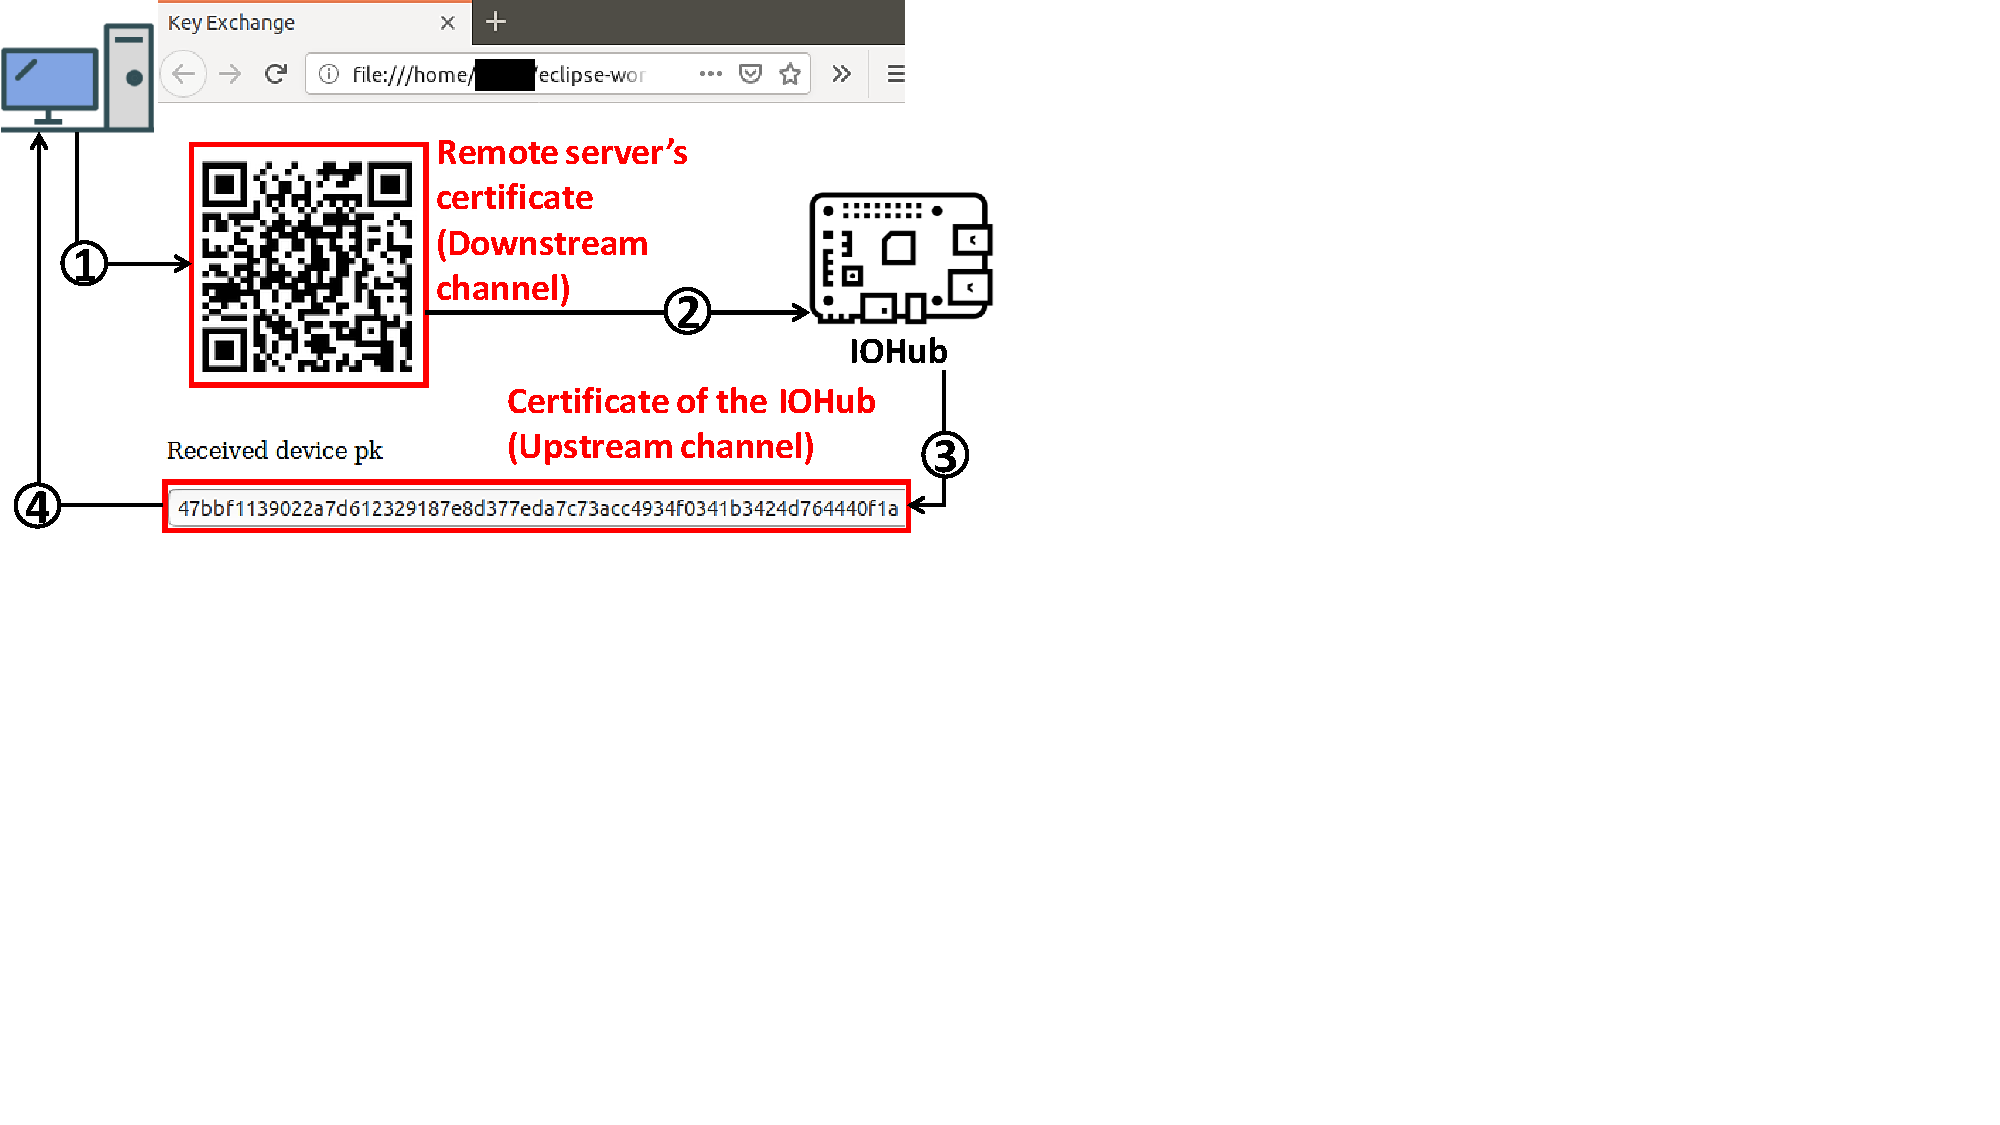
\includegraphics[trim={0 10cm 17cm 0}, clip, width=0.85\linewidth]{keyExchange_1.pdf}
\caption{\textbf{Establishing \tls.} A snapshot of the key exchange web page that is used to communicate the public certificates of the device and the remote server.}
%\spacesave
\label{fig:keyExchange}
\centering
\end{figure} 

\myparagraph{Establishing \tls}
\label{sec:prototype:impl:tls}
%
For the IO confidentiality, the \device and server create a \tls channel. When the user opens up a secure webpage, key exchange is the first step that takes place. We assume that the remote server already has the \device's certificate, or some offline registration takes place. An instance of the key exchange protocol of \name is illustrated in Figure~\ref{fig:keyExchange}. The flow of the key exchange mechanism is as the following:
%\vspace{-10pt}
\begin{mylist}
  \item[\one] The server delivers a web page with a QR code that encodes the signed public key of the server (server hello in TLS). 
  \item[\two] The device captures every frame until it detects a QR code. Then, it decodes the QR code and verifies the public key and derives the shared secret using Diffie-Hellman protocol~\cite{blake1998authenticated}. 
  \item[\three] The device then sends its signed public certificate to the host, which forwards it to the server.
  \item[\four] The remote server gets the signed certificate from the \device, verifies it, and finally derives the shared secret.
\end{mylist}

\begin{figure}[t]
\centering
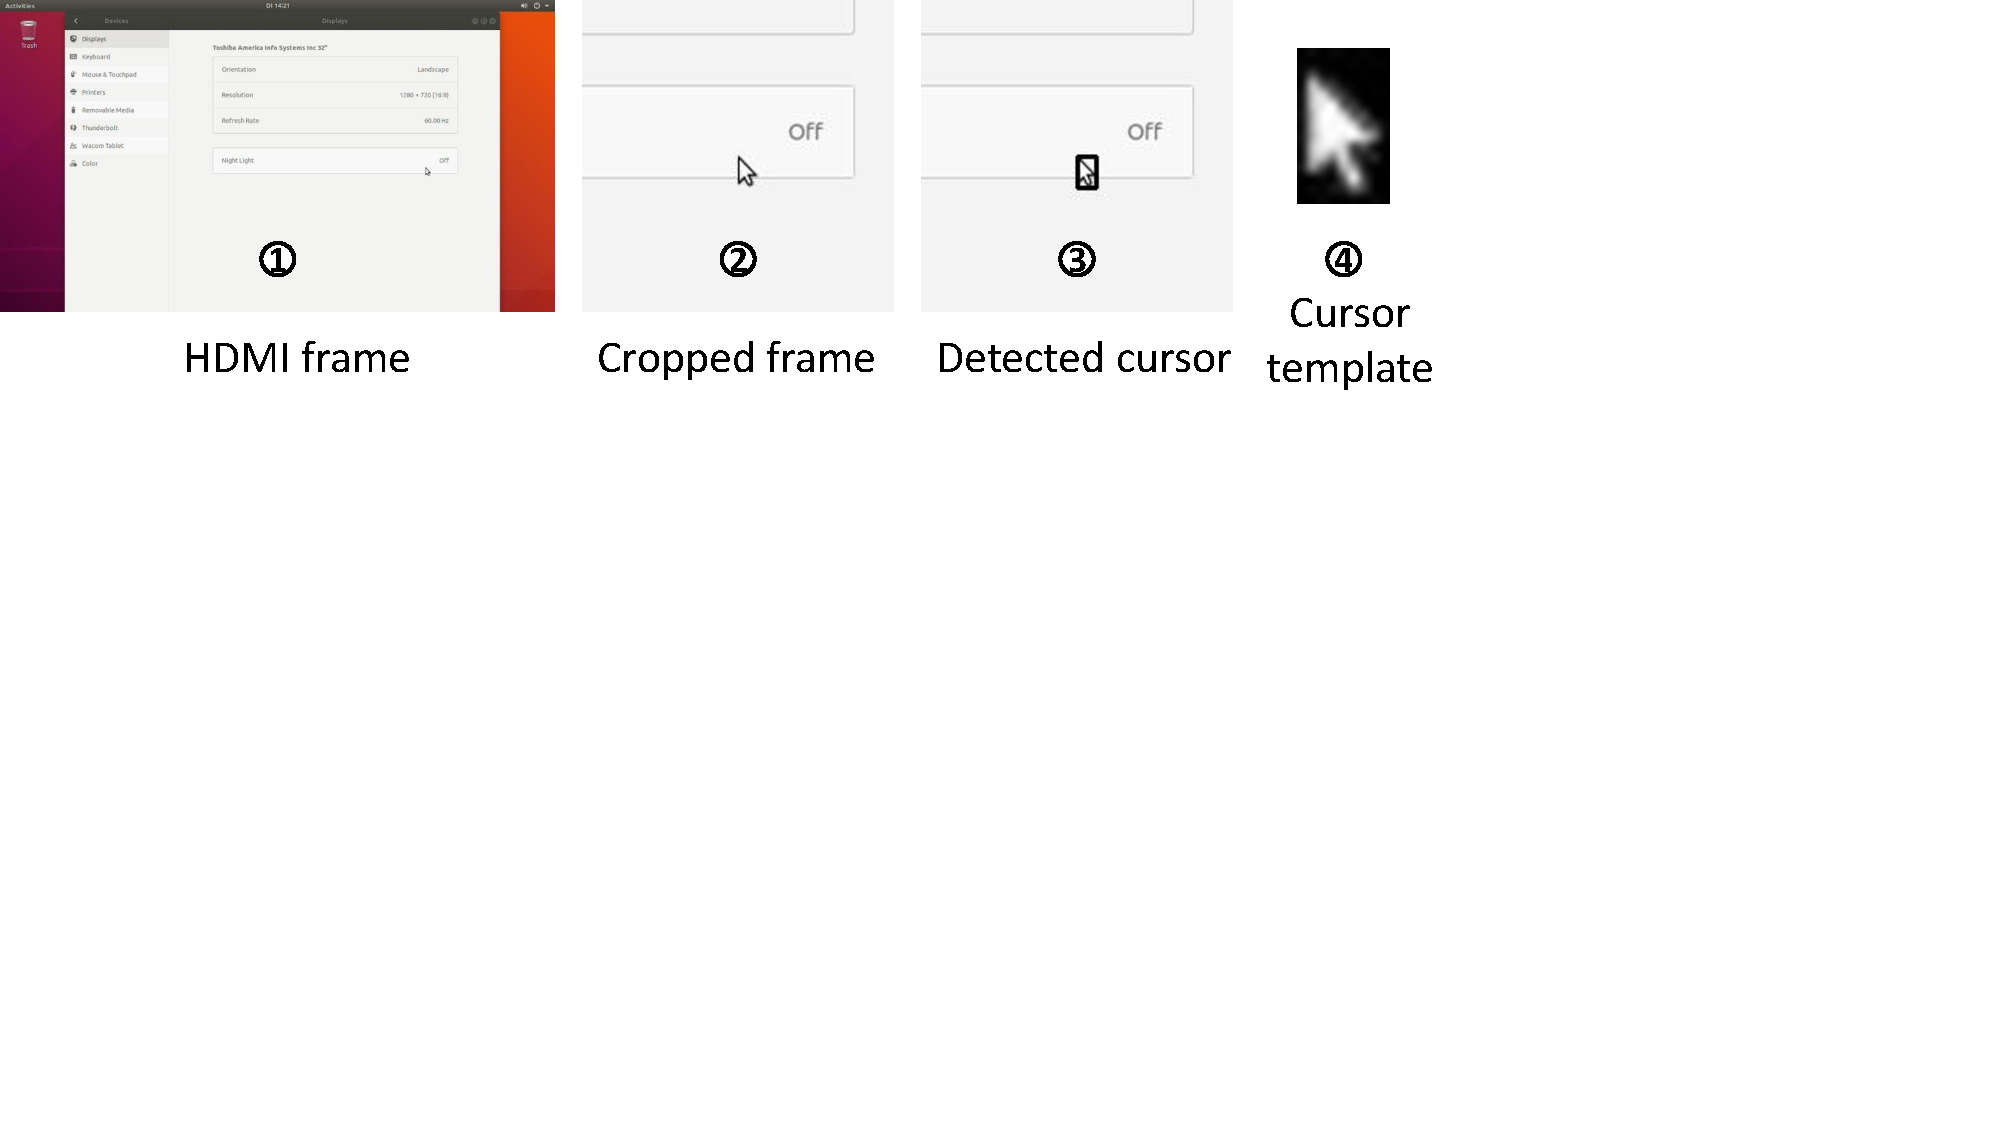
\includegraphics[trim={0 12cm 10cm 0}, clip, width=\linewidth]{cursorDetect.pdf}
\caption{\textbf{Cursor detection on the HDMI frame.} The figure shows \name mouse pointer tracking. \one shows the captured HDMI frame captured by B101 HDMI to CSI bridge. \two shows the cropped HDMI frame based on the mouse position received by the \device. \three shows the detected mouse pointer. For testing, we program the \device to put a rectangle around the pointer. \four shows one of the pointer templates that we used in our OpenCV routine.}
%\spacesave
\label{fig:cursorDetect}
\centering
\end{figure} 


\myparagraph{HID Drivers}
We use Arduino prototype development board as the HID drivers. Figure~\ref{fig:prototype} shows an Arduino Due, and a Zero board where the Due connects to the HIDs via the native USB port and the Zero relays the HID data to the Raspberry Pi (RPi). The Due and the Zero boards are connected over $I^2C$ interface. As both Due and Zero only have one native USB port on each of them, we were forced to use two boards as an HID interceptor and relay. The Zero relays the HID signals both to the connected host (over native USB) and to the RPi (over serial interface). The connection from the Zero to the host is one way and emulates a composite HID. While the connection between the Zero and the RPi is bidirectional. The HID drivers are implemented using the native Arduino \texttt{keyboard} and \texttt{mouse} library. On the RPi, no HID drivers were needed as the RPi receives processed HID data from the Zero (for the pointer: displacement over x and y-axis and for keyboard, ASCII characters).


\myparagraph{HDMI Interceptor, Relay and Overlay}
The RPi along with the Auvidea B101 HDMI to CSI bridge, acts as the HDMI interceptor and relay. The B101 board converts HDMI signals from the host as a camera input (via the CSI interface) to the RPi. This allows the RPi to access the HDMI frames as a stream of JPEG frames. The HDMI out of the RPi acts as the relay that connects to the monitor. On the RPi, we use Picamera API~\cite{picamera} to access the HDMI frames. The B101 is capable of processing 25 frames at 1080p resolution. Hence, this is the hardware bottleneck of our implementation. However, the upcoming B112 board
%\footnote{still in development: \url{https://auvidea.eu/showcase/}.} 
could solve this performance issue.

On the RPi, the overlay and HDMI out is implemented using Java SWT. Using SWT, we create a full-screen window that is shown on the monitor. The SWT class polls the HDMI frames and process them as individual JPEG images via the \texttt{BufferedImage} class. This allows the overlays to be drawn on the HDMI images efficiently. The Java program uses a QR code interpreter to extract the UI specification. Based on the UI specification, it creates the geometrical shapes (corresponding to the UI elements) and draw them on the frames. In the current implementation of the \name, the UI elements such as button, text-field, radio button etc. are preloaded in the \device memory. Note that the current implementation of \device is based on the RPi. But one could implement such functionality on an FPGA, reducing the TCB even more. 


\myparagraph{Mouse Pointer Tracking}
The pointer tracing is also executed in the aforementioned Java program using simple object detection technique suppled by the OpenCV API. Figure~\ref{fig:cursorDetect} shows one screenshot of the pointer detection. The Figure shows the entire HDMI frame, the cropped frame of resolution $200 \times 200$ px (based on the mouse input data), the detected pointer in the cropped frame and the cursor template that is used by the object detection algorithm.





\end{document}

